\documentclass[a4paper,12pt,twoside]{article}
%% Language and font encodings
\usepackage[chinese]{babel}
\usepackage{fontspec}
\usepackage[UTF8]{ctex}
\usepackage{float}
%% Sets page size and margins
\usepackage[a4paper,top=2cm,bottom=2cm,left=2.1cm,right=2.1cm,marginparwidth=2cm]{geometry}
\usepackage{titlesec}  %目录
\usepackage{titletoc}  %目录
%% Useful packages
\usepackage{amsmath,amsthm,amssymb,amsfonts}
\usepackage{array}
\usepackage{graphicx}
\usepackage{subfigure}
\usepackage[colorinlistoftodos]{todonotes}
\usepackage[style=numeric,sorting=none]{biblatex}
\usepackage[colorlinks=true, allcolors=blue]{hyperref}
\usepackage{listings}
\usepackage{booktabs}
\usepackage{verbatim}
\usepackage{fancyhdr}
\usepackage{mhchem}
\usepackage{ctexcap}
\usepackage{tikz}
\usepackage{enumitem}
\setenumerate[1]{itemsep=0pt,partopsep=0pt,parsep=\parskip,topsep=5pt}
\setitemize[1]{itemsep=0pt,partopsep=0pt,parsep=\parskip,topsep=5pt}
\setdescription{itemsep=0pt,partopsep=0pt,parsep=\parskip,topsep=5pt}
\CTEXoptions[bibname={\large {参考文献}}]
\usepackage{bibspacing}
\setmainfont{Times New Roman}
\pagestyle{fancy}
 
\fancyhf{}
\fancyhead[OR]{\fangsong{高频电子线路 INFO130029.01\quad 2022\quad 课程报告:FM收音机设计}}
\fancyhead[EL]{\fangsong{ 苏浩阳 \quad \leftmark}}
\title{\vspace{-1.5cm}FM收音机电路设计及其仿真}
\author{20300720002 苏浩阳}
\date{}

\addbibresource{r.bib}

\begin{document}

\maketitle
\section{设计方案概述}
\subsection{设计指标与参数}
FM收音机设计过程主要考虑可接纳的载波频率范围$f_{0}$,中频$f_{I}$,音频信号带宽范围及灵敏度。

\begin{itemize}
\setlength{\itemsep}{0pt}
\setlength{\parsep}{0pt}
\setlength{\parskip}{0pt}
    \item [$\bullet$]调频收音机从天线接受已调信号,由于调制信号载波频率为88MHz-108MHz,收音机工作频率与无线电波频率相对应,因此工作频率范围$f_0$从88MHz到108MHz;
    \item [$\bullet$]由调频收音机标准,采用中频10.7MHz;
    \item [$\bullet$]声音带宽10kHz,即音频信号(基带)频率范围从0Hz附近至10kHz;
    \item [$\bullet$]灵敏度不低于$10\mathrm{\mu V}$,即鉴频跨导(S曲线载波频率位置斜率)不低于$10\mathrm{\mu V}$。
\end{itemize}

\subsection{FM收音机系统框图}
FM收音机主要由高放级,变频级、解调及低放级构成\cite{1}。高放级包含输入回路及高频放大;变频级包含混频、本振与AFC控制、中放,解调即鉴频电路;低放级含低频放大及低频功放。
\begin{figure}[H]
    \centering
    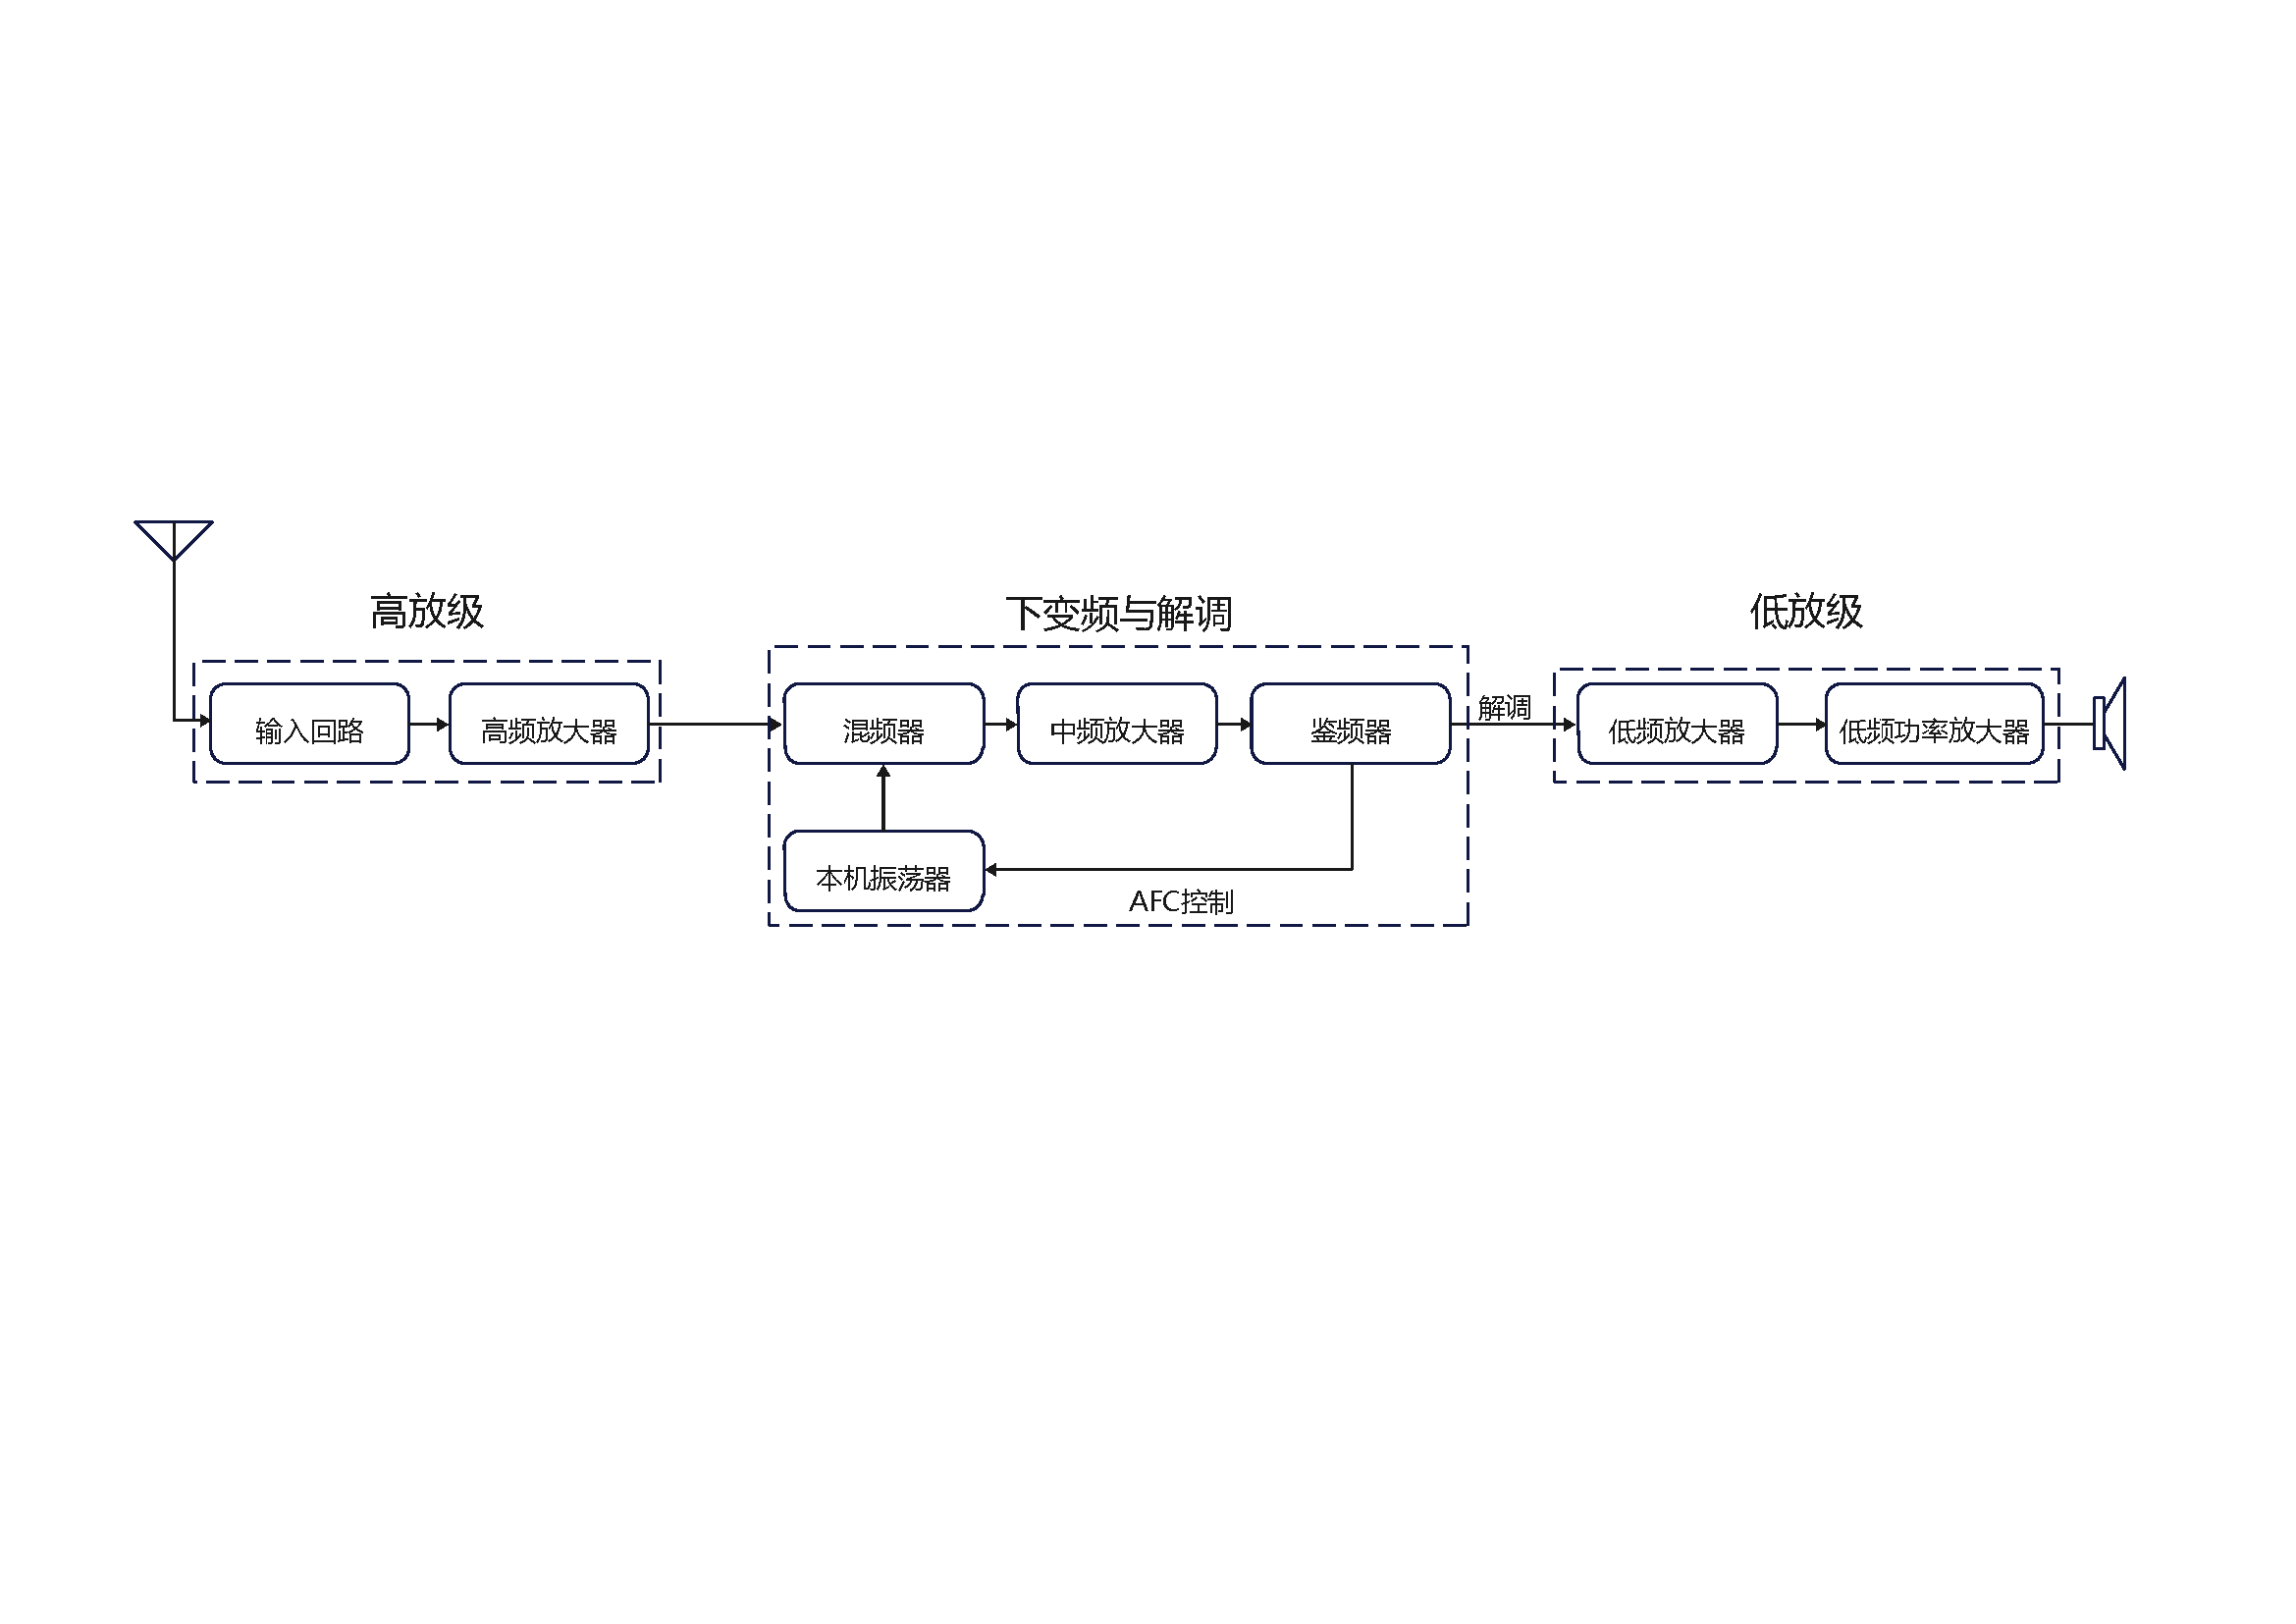
\includegraphics[scale=0.45]{FM系统框图.pdf}
    \caption{FM收音机系统框图}
    \label{FM框图}
\end{figure}
\subsection{工作过程}
在高放级,FM收音机通过天线接受已调波,其载波频率介于88MHz至108MHz之间,通过输入调谐回路选频滤除载波频率以外的频率分量,剩余频率信号进入高放电路放大,并经高放电路负载的同步调谐回路,进一步滤除干扰信号。

在变频级,混频器接收高放级选出的频率$f_{S}$,与本机振荡产生的大信号$f_{L}$混频实现下变频,得到中频信号$f_{I} = f_L-f_S$。变频过程中使载波频率变为10.7MHz,不改变调频波中音频信号引起的频偏。

中频信号经中频放大电路放大及选频,输出信号送至鉴频器解调。解调器从已调信号中选出音频信号,最后通过低放级放大送入扬声器。

\section{电原理图与参数设计}
\subsection{高放级}
\subsubsection{输入调谐回路设计}
为了增强收音机接受天线信号时的抗干扰能力,通过在输入级增设一个调谐回路以提高天线回路的Q值\footnote{谐振频带宽度应当允许在中心频率附近含有最大频偏的调频波通过,而超过范围的频率要被滤除,但品质因数有上限$Q_0$,因此带宽不可能一直缩小以满足要求,因此采用两级谐振 回路将超过频偏范围的信号二次滤除。}。

如图\ref{输入头}所示,$C_1,C_2,L_1$构成可调谐回路,其中$C_1$为可变电容,电容取值约为1pF至6pF,$C_2$与之并联,假定$C_2$电容值固定为10pF,选用$0.2\mathrm{\mu H}$电感$L_1$。
    
    上述取值下,谐振频率
    \begin{equation}
        f_{0}=\frac{1}{2\pi \sqrt{(C_1+C_2)\cdot L_1}}\in [88\mathrm{MHz},108\mathrm{MHz}]
        \label{1式}
    \end{equation}

  \begin{figure}[H]
        \centering
        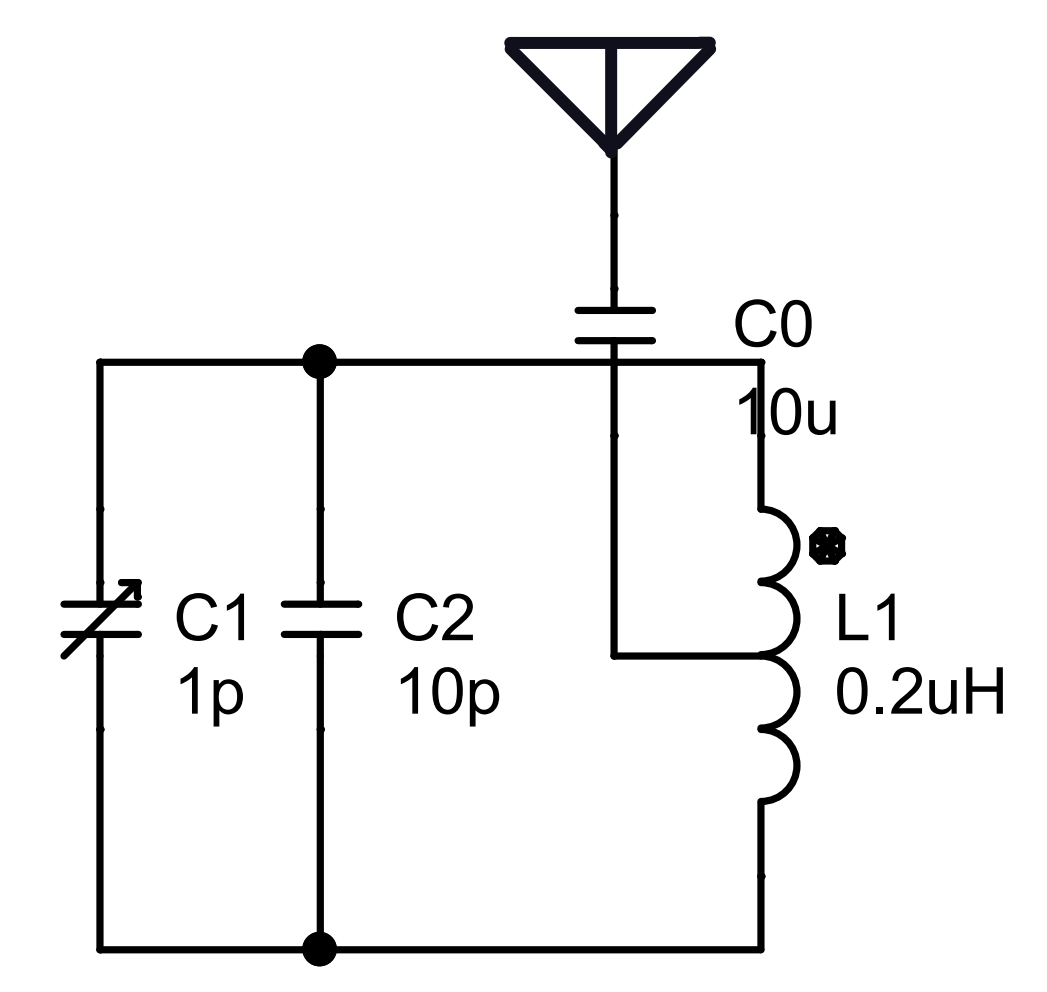
\includegraphics[scale=0.1]{输入头.png}
        \caption{可调谐输入回路电原理图}
        \label{输入头}
    \end{figure}




\subsubsection{高频小信号放大电路设计}
高频小信号放大器要求增益高、噪声系数低,可选用晶体管放大器或场效应管放大器提高信噪比。但考虑到前级已增加一级调谐回路用以选频,且由于场效应管跨导小,在提高增益上有局限性,因此采用一级晶体管放大器进行设计。

此外,选用恰当的静态工作点,晶体管的高电流放大系数能够更好地提高天线输入信号的功率。

在负载端,选用LC并联谐振回路起选频作用;为保证阻抗匹配条件,采用传输线变压器与后级耦合\cite{罗伟雄2003调频收音机评述}。

\textbf{[设计流程]}
\begin{itemize}
    \item 静态工作点设置:根据FM收音机功率标准,选用集电极偏置电压$V_{CC}=5\mathrm{V}$,基极电压$V_{BB}=3\mathrm{V}$。为减小晶体管输入阻抗对前级调谐回路阻抗匹配关系带来的影响,选用较大的偏置电阻$R_{b1},R_{b2}$。由表达式$V_{BB}=\frac{R_{b1}}{R_{b1}+R_{b2}}\cdot V_{CC}$,采用$R_{b1}=30\mathrm{k}\Omega,R_{b2}=20\mathrm{k}\Omega$。根据经验值,选用射极电阻$R_{e1}=1\mathrm{k}\Omega$。电原理图如图\ref{直流}所示。
    \begin{figure}[H]
        \centering
        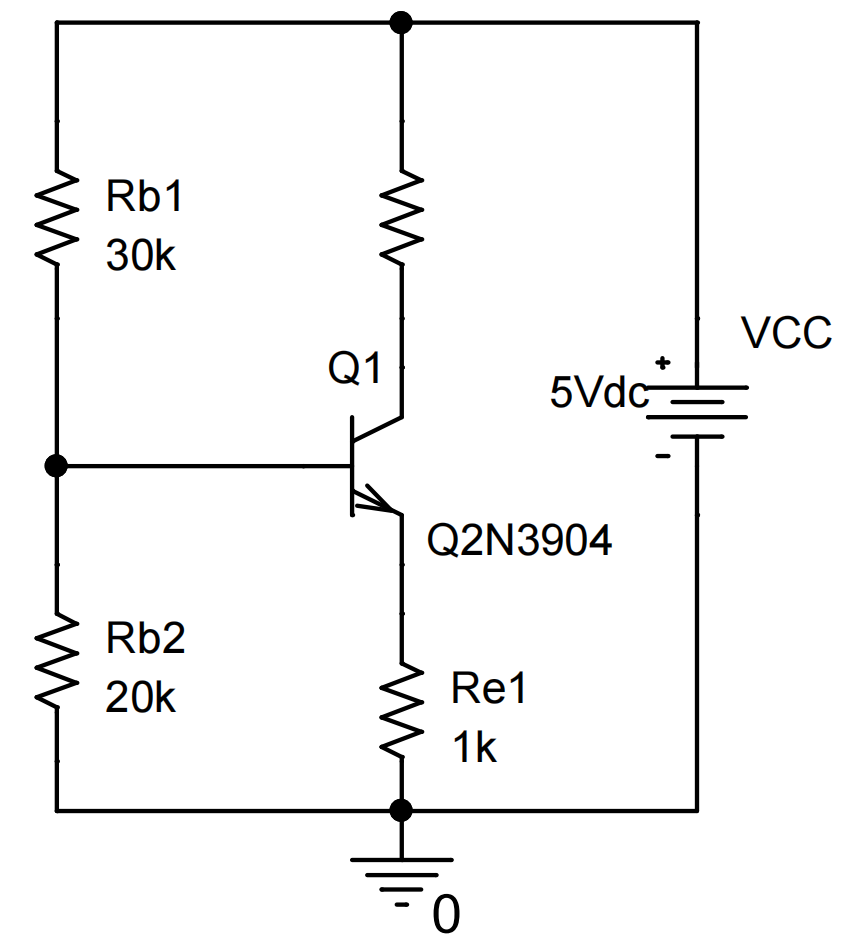
\includegraphics[scale=0.13]{直流通路.png}
        \caption{高频小信号放大器直流通路电原理图}
        \label{直流}
    \end{figure}
    \item 选频网络设计:由于FM收音机接收频率随着天线输入频率的改变而改变,因此采用可调谐的谐振回路结构。由于高放级的输入与输出回路均用于对天线载波频率进行选择,因此输出调节回路的设计过程与输入调谐回路类似,电路如图\ref{小信号sch}所示。
    
    \begin{figure}[H]
        \centering
        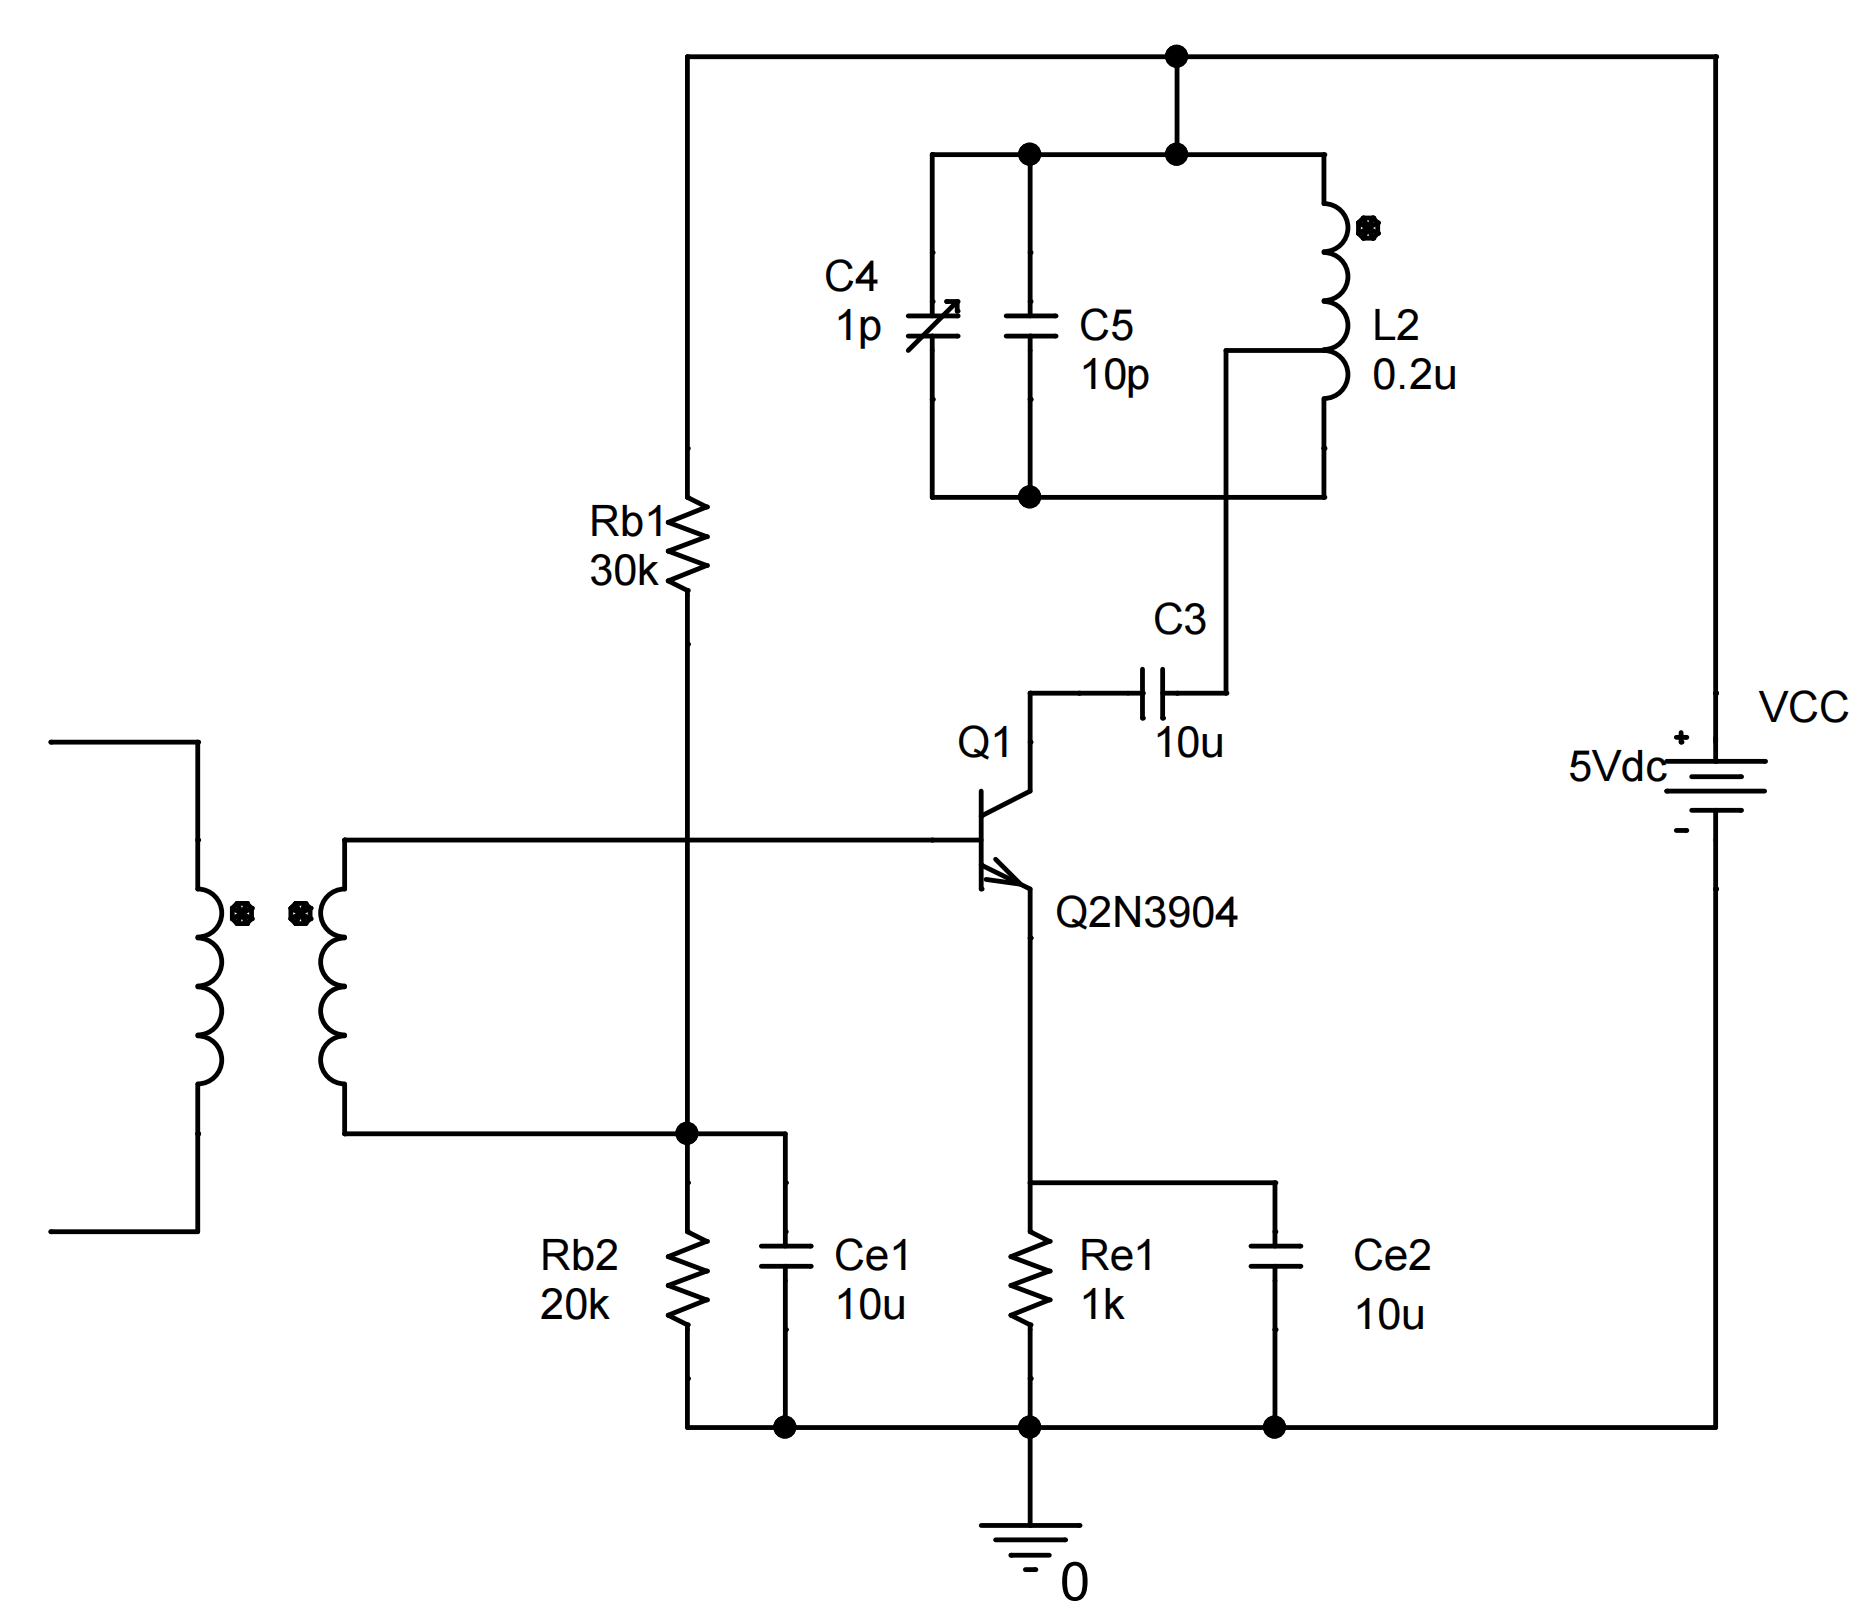
\includegraphics[scale=0.12]{小信号放大器sch.png}
        \caption{高频小信号放大器电原理图}
        \label{小信号sch}
    \end{figure}
\end{itemize}

$C_{e1}$及$C_{e2}$为直流耦合及旁路电容。电容$C_4$与输入回路的电容$C_1$构成双联电容,以同步改变谐振频率。

对高放级谐振回路,可变电容$C_4$,固定电容$C_5$与电感$L_2$的参数设计与输入回路一致。其中晶体管集电极以抽头接入电感。

\subsection{混频级}

\subsubsection{本机振荡器设计}
\textbf{[谐振回路设计]}

考虑到接收频率$f_{S}$范围变化较大,为了产生固定的中频 $f_I$,选用带有可变电容的Seiler振荡器作为本机振荡器(如图\ref{本振sch}),以改善调节频率的方便性。
\begin{figure}[H]
    \centering
    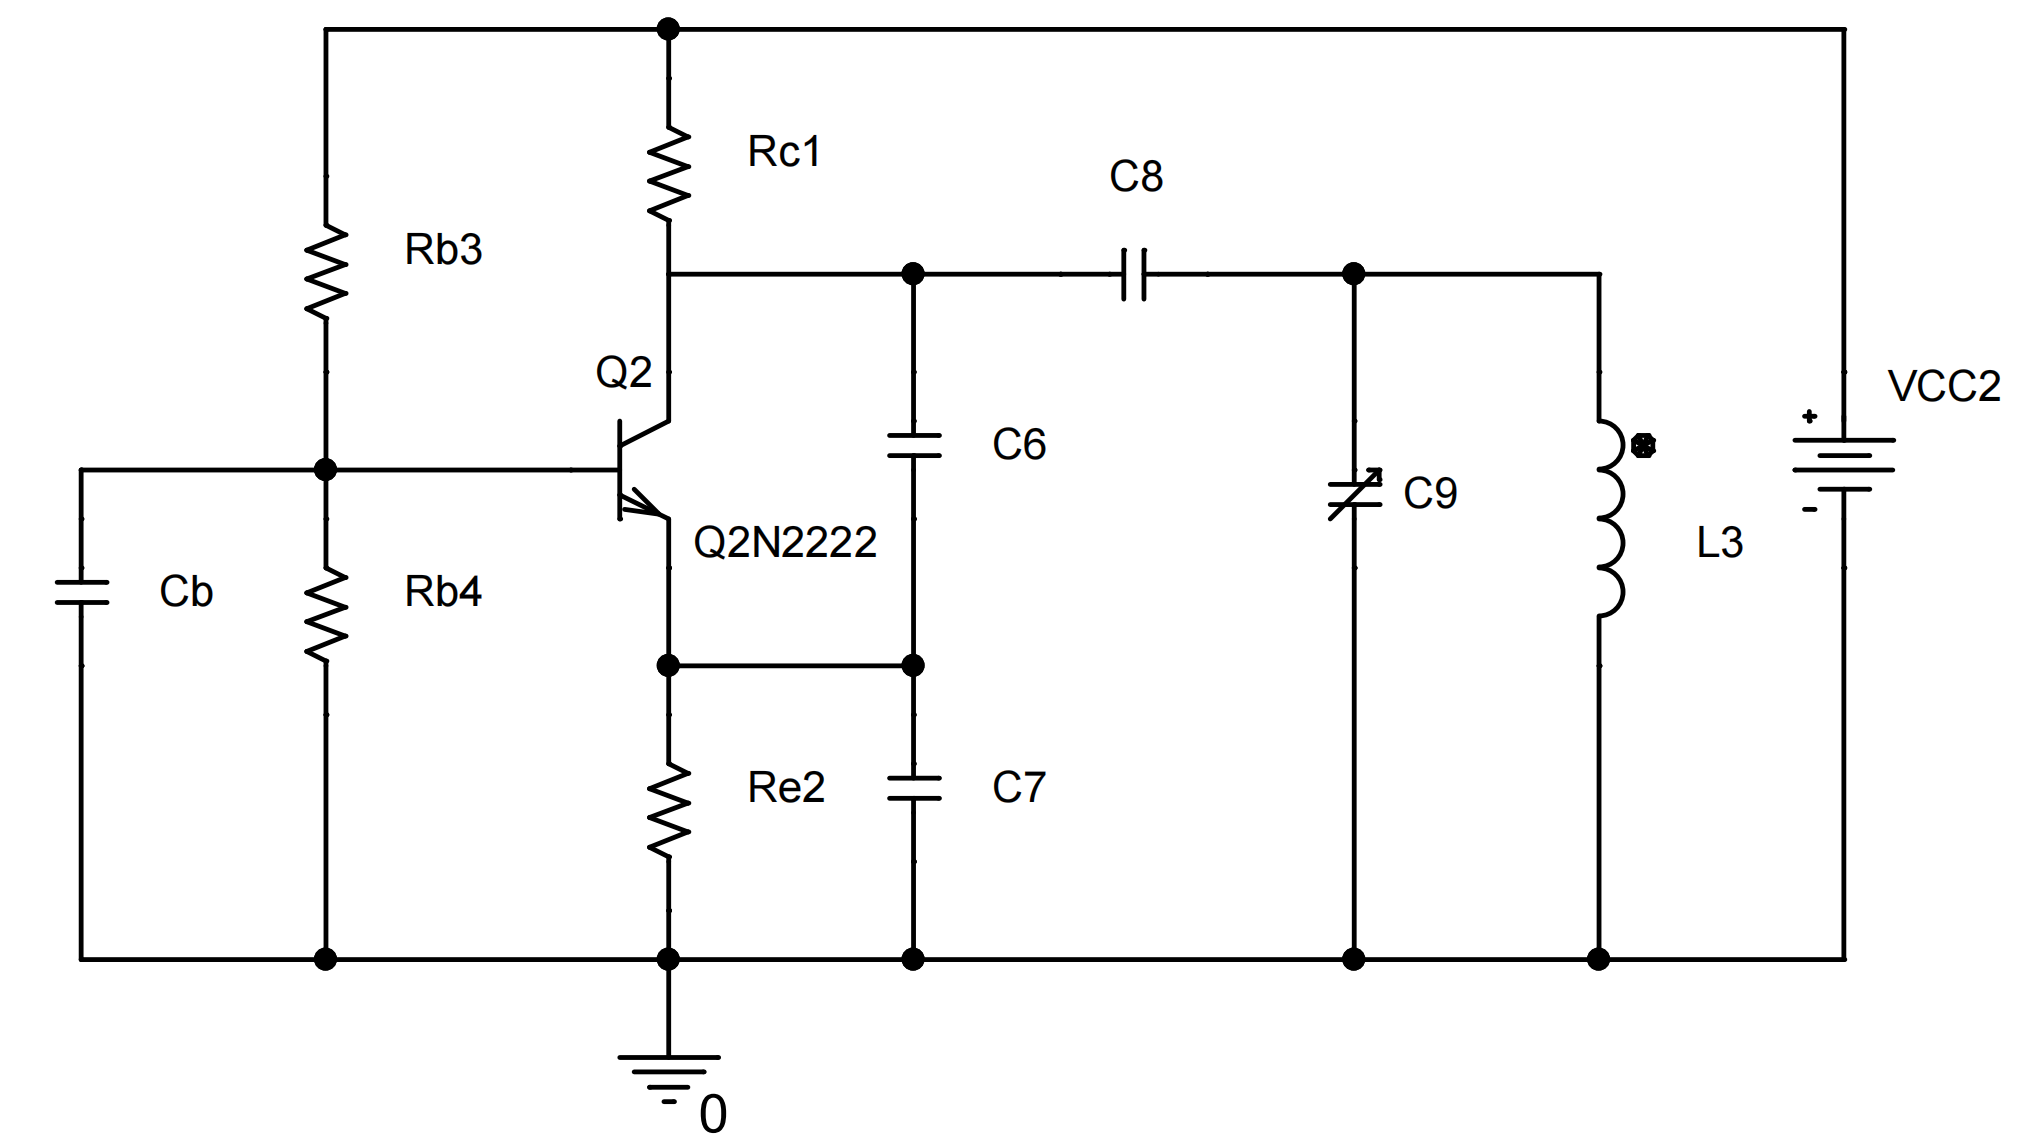
\includegraphics[scale=0.125]{本振待调参原理图.png}
    \caption{本机振荡器电原理图}
    \label{本振sch}
\end{figure}
考虑到本机振荡器的起振条件与晶体管参数相关,通过查阅仿真器件手册\cite{2},得到选用的晶体管Q2N2222相关电容参数\footnote{表中$C_{je}$代表发射结势垒电容,$C_{jc}$代表集电结势垒电容。}如表\ref{Q2N2222}所示。
\begin{table}[H]
    \centering
    \begin{tabular}{cccc}
    \toprule[2pt]
      model Q2N2222 (NPN)  &  $C_{\mathrm{j}e}$&$C_{\mathrm{j}c}$ \\
      \midrule[1pt]
        模型参数值  &22.01pF &7.306pF \\
        \bottomrule[2pt]
    \end{tabular}
    \caption{仿真晶体管Q2N2222电容参数值}
    \label{Q2N2222}
\end{table}

根据晶体管参数设计经验,一般有
\begin{equation}
    \begin{aligned}
    C_{i} &\approx C_{\pi}=C_{\mathrm{j}e} \\
    C_o &\approx C_{\mu} = C_{\mathrm{jc}}\\
    \end{aligned}
\end{equation}
此处发射结电容$C_{\pi}$与集电结电容$C_{\mu}$分别构成了晶体管的输入电容与输出电容。



由于Seiler振荡器的反馈系数F只由固定电容$C_6,C_7$及晶体管输入电容决定,为了避免晶体管产生波形失真,同时又要增加晶体管起振的容易度,反馈系数F通常取值介于0.1至0.5之间,由反馈系数表达式
\begin{equation}
    |F(\mathrm{j}\omega)|=\frac{v_e}{v_c}\approx \frac{C_6}{C_6+C_7+C_{i}}
\end{equation}
另一方面,为了减小晶体管极间电容取值对反馈系数的影响,可选用高于$C_i$参数的电容$C_6$。

基于以上两点讨论,若选取$|F(\mathrm{j}\omega)|=0.42$,$C_6=30\mathrm{pF}$,则
\begin{equation}
    \begin{aligned}
    C_7=&(\frac{1}{F}-1)\cdot C_6-C_i\\
    =&(\frac{1}{0.42}-1)\cdot 30 - 22.01\approx 18\mathrm{pF}\\
    \end{aligned}
\end{equation}
对FM收音机的本机振荡器而言,其振荡频率较高,达约98.7MHz至118.7MHz,可选取较小的电容值$C_8=4\mathrm{pF}$,以使总电容$C_\Sigma$减小。


为了避免本机振荡器产生间歇振荡,需要提高回路的有载品质因数Q,由谐振回路表达式
\begin{equation}
    Q = \frac{1}{G\cdot\rho}=\frac{1}{G\cdot \omega_0 L}
\end{equation}
可知,电感L设计值不能过高,选用$L = 0.6\mathrm{\mu H}$。

由于电容$C_6,C_7$取值较大,从而极间电容影响较小,谐振回路总电容$C_{\Sigma}$取值近似为
\begin{equation}
    C_{\Sigma}\approx C_9 + \frac{C_6 C_7 C_8}{C_6C_7+C_7C_8+C_6C_8}
\end{equation}
当满足
\begin{equation}
    98.7\mathrm{MHz} \le f_{L}=\frac{1}{2\pi \sqrt{L\cdot C_\Sigma}}\le 118.7\mathrm{MHz}
    \label{7式}
\end{equation}
则
\begin{equation}
    C_9 = \frac{1}{L_3\cdot (2\pi f_L)^2}-\frac{C_6 C_7 C_8}{C_6C_7+C_7C_8+C_6C_8}
    \in (0.03,1.44)\mathrm{pF}
\end{equation}

\vspace{2pt}
\textbf{[静态工作点选取]}

静态工作点的选取决定了本机振荡器的工作点电流$I_{CQ}$,为了使得本机振荡器能够起振,工作点电流应当大于最小起振电流$I_{C_{min}}$。'

即满足
\begin{equation}
    \begin{aligned}
    I_{CQ} > I_{C_{min}}=&g_{m_{min}}\cdot V_{T} = (\frac{1}{p}\cdot (\frac{1}{r_{ce}}+g_0)+p\cdot (g_{m_{min}}+\frac{1}{R_{e2}})) \cdot V_{T}\\
    \end{aligned}
\end{equation}
 其中p为接入系数,有$p=\frac{C_6}{C_6+C_7+C_i}$。

由前述讨论,若仅考虑谐振回路电感的损耗,则损耗电导$g_0\approx 131\mathrm{\mu S}$,假设热电势$V_{T}=26\mathrm{mV}$,选取较小的射极偏置电阻$R_{e2}=250\Omega$,忽略$r_{ce}$的影响,则$g_{m_{min}}=0.36\mathrm{mS}$,有$I_{CQ}>9.36\mathrm{\mu A}$。一般而言,工作点电流设置为远高于最小起振电流,对本机振荡器,可设定$I_{CQ}$为毫安级。

本机振荡器参数设计如图\ref{本振参数}所示:
\begin{figure}[H]
    \centering
    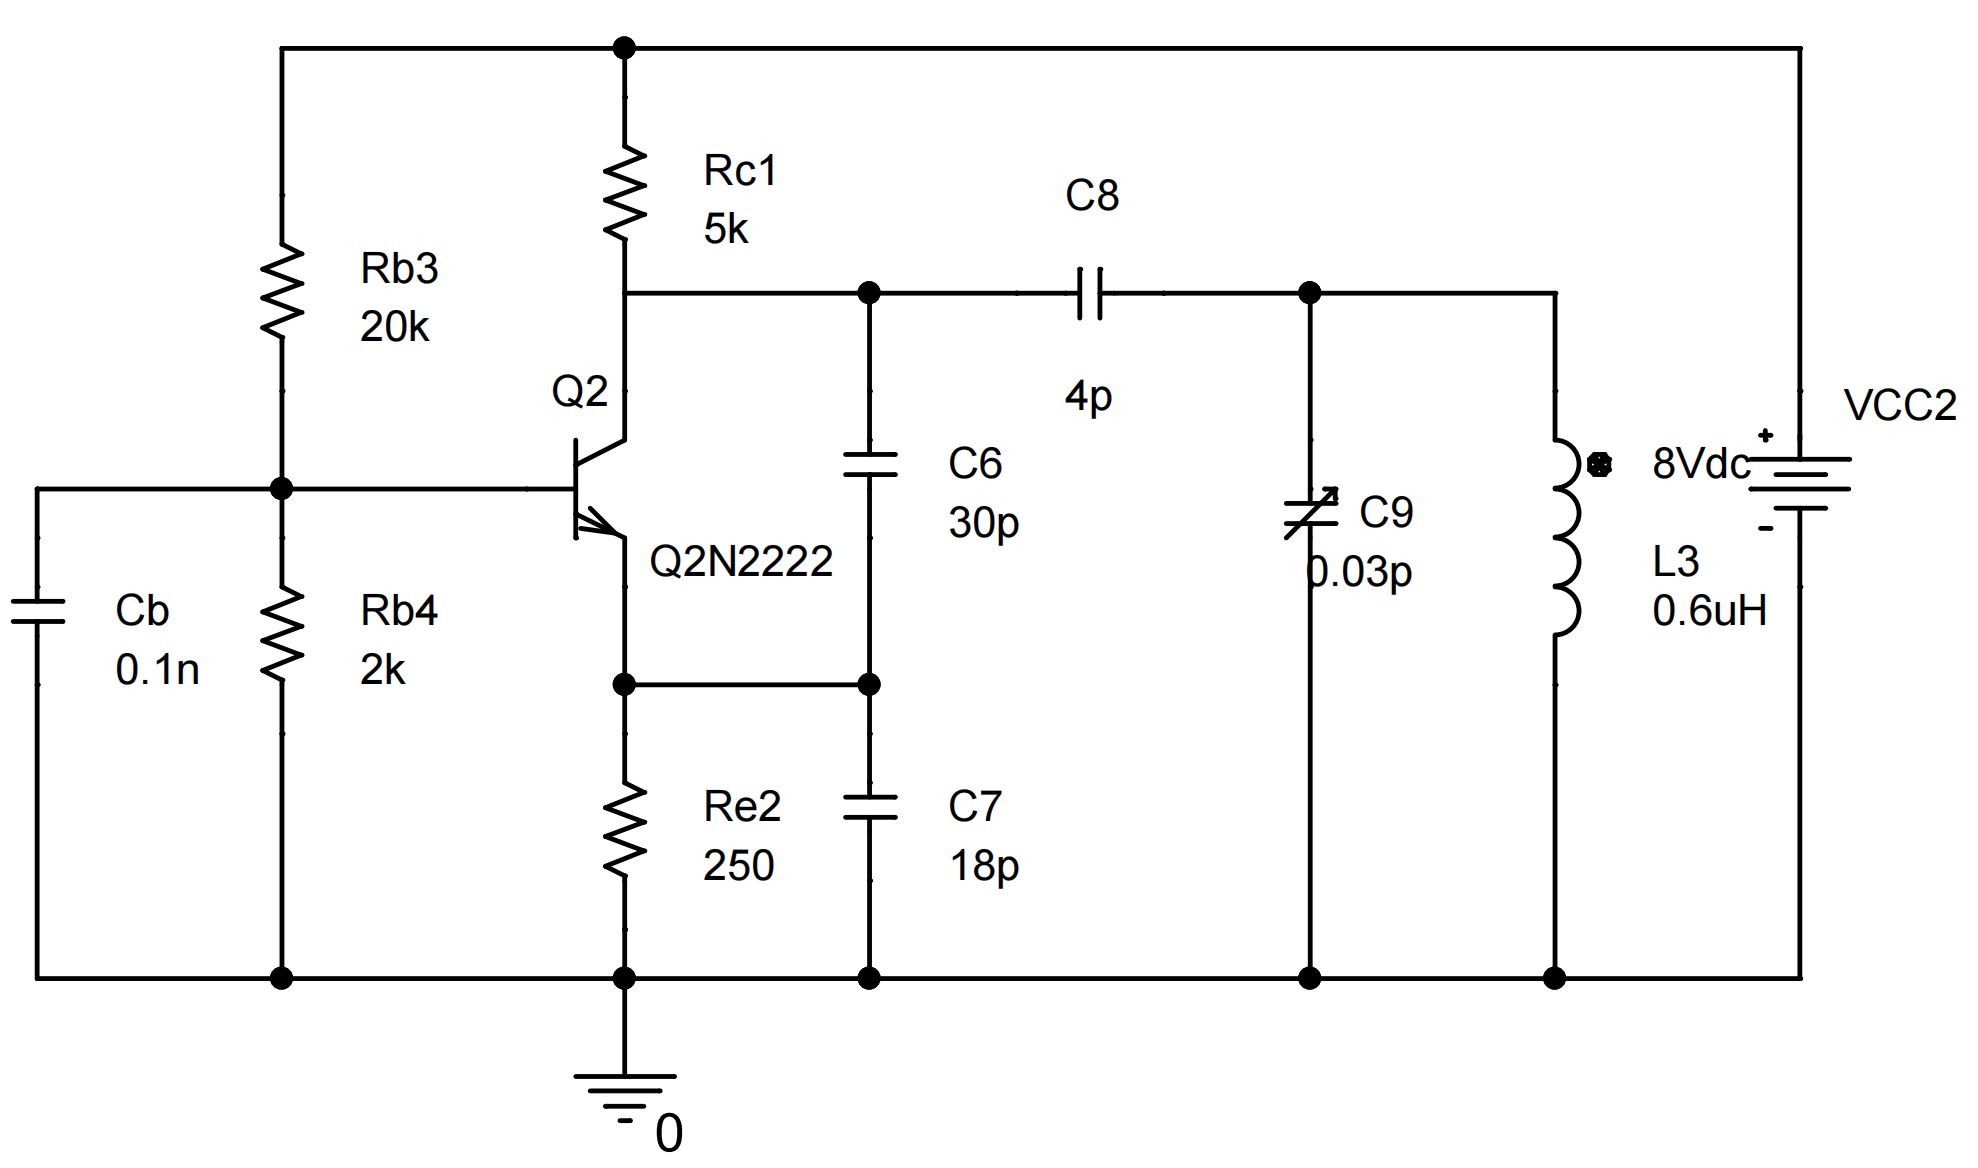
\includegraphics[scale=0.125]{本振电路sch已调参.png}
    \caption{本机振荡器参数设计电原理图}
    \label{本振参数}
\end{figure}

\subsubsection{混频器设计}
\textbf{[中频频率的选择]}

混频器的负载谐振回路应谐振在中频,对FM收音机,一般取10.7MHz作为中频,以下首先验证选择中频$f_{I}=10.7\mathrm{MHz}$的合理性。

由于混频器是非线性电路,因此在混频过程中会产生额外的n次频率成分$f_{(n)}=|pf_{1}+qf_2|_{p+q=n}$,对高阶分量($n\ge 3$),可以通过电路改进以减少高阶产物;对二阶分量,尤其是镜像频率$f_{MR}$,需要选择恰当的谐振中频,使镜像频率$f_{MR}$下的信号衰减。

具体地,镜像频率$f_{MR}$与接收频率$f_{S}$间隔两个中频频率的宽度,由前述设计可知,本振频率$f_{L}=f_{S}+f_{I}$,从而$f_{MR}=f_{L}+f_{I}$。因此问题转化为,要求以$f_{S}$为中心的通频带有足够好的选择性,确保镜像频率落在选择范围之外。

在高放级设计中,已同时采用输入调谐以及小信号放大极调谐回路,因此幅频特性可表示为:
\begin{equation}
    |H(\mathrm{j}\omega)|_{\Sigma}=\frac{1}{|1+\mathrm{j}\xi|^2}
\end{equation}
若要求输出镜像频率在从天线端进入至混频器的过程中,幅度衰减至60dB,假设有载Q值为80,并以最大接收频率108MHz带入,则
\begin{equation}
    \begin{aligned}
  & \frac{1}{|1+\mathrm{j}\xi|^2}=\frac{1}{10^{\frac{60}{20}}}
    \Rightarrow\xi=\sqrt{999}\approx 31.6\\
    \Rightarrow & BW_{-60dB}=\xi \cdot\frac{f_S}{Q_L}=31.6\times \frac{108\times 10^6}{80}=42.66\mathrm{MHz}\\
    \Rightarrow & f_{I} =  \frac{BW_{-60dB}}{4}=\frac{42.66}{4}=10.665\mathrm{MHz}
    \end{aligned}
\end{equation}
上式表明,中频频率只要达到10.665MHz,就能将镜像频率干扰衰减至60dB以下,若选择中频频率$f_I=10.7\mathrm{MHz}>10.665\mathrm{MHz}$,则能将二阶频率干扰分量滤除;另一方面,由于中频$f_{I}=10.7\mathrm{MHz}$不在高放级放大频率范围之内,即
\begin{equation}
    f_{I}=10.7\mathrm{MHz} \notin (f_{S_{min}}-2f_{I},f_{S_{max}}+2f_{I})=(66.6\mathrm{MHz},129.4\mathrm{MHz})
\end{equation}
选频效果如图\ref{中频选择图形}所示,因此中频频率不会绕过混频级,即不会成为干扰。从以上两个角度,FM收音机选择10.7MHz作为中频是合理的。
\begin{figure}[H]
    \centering
    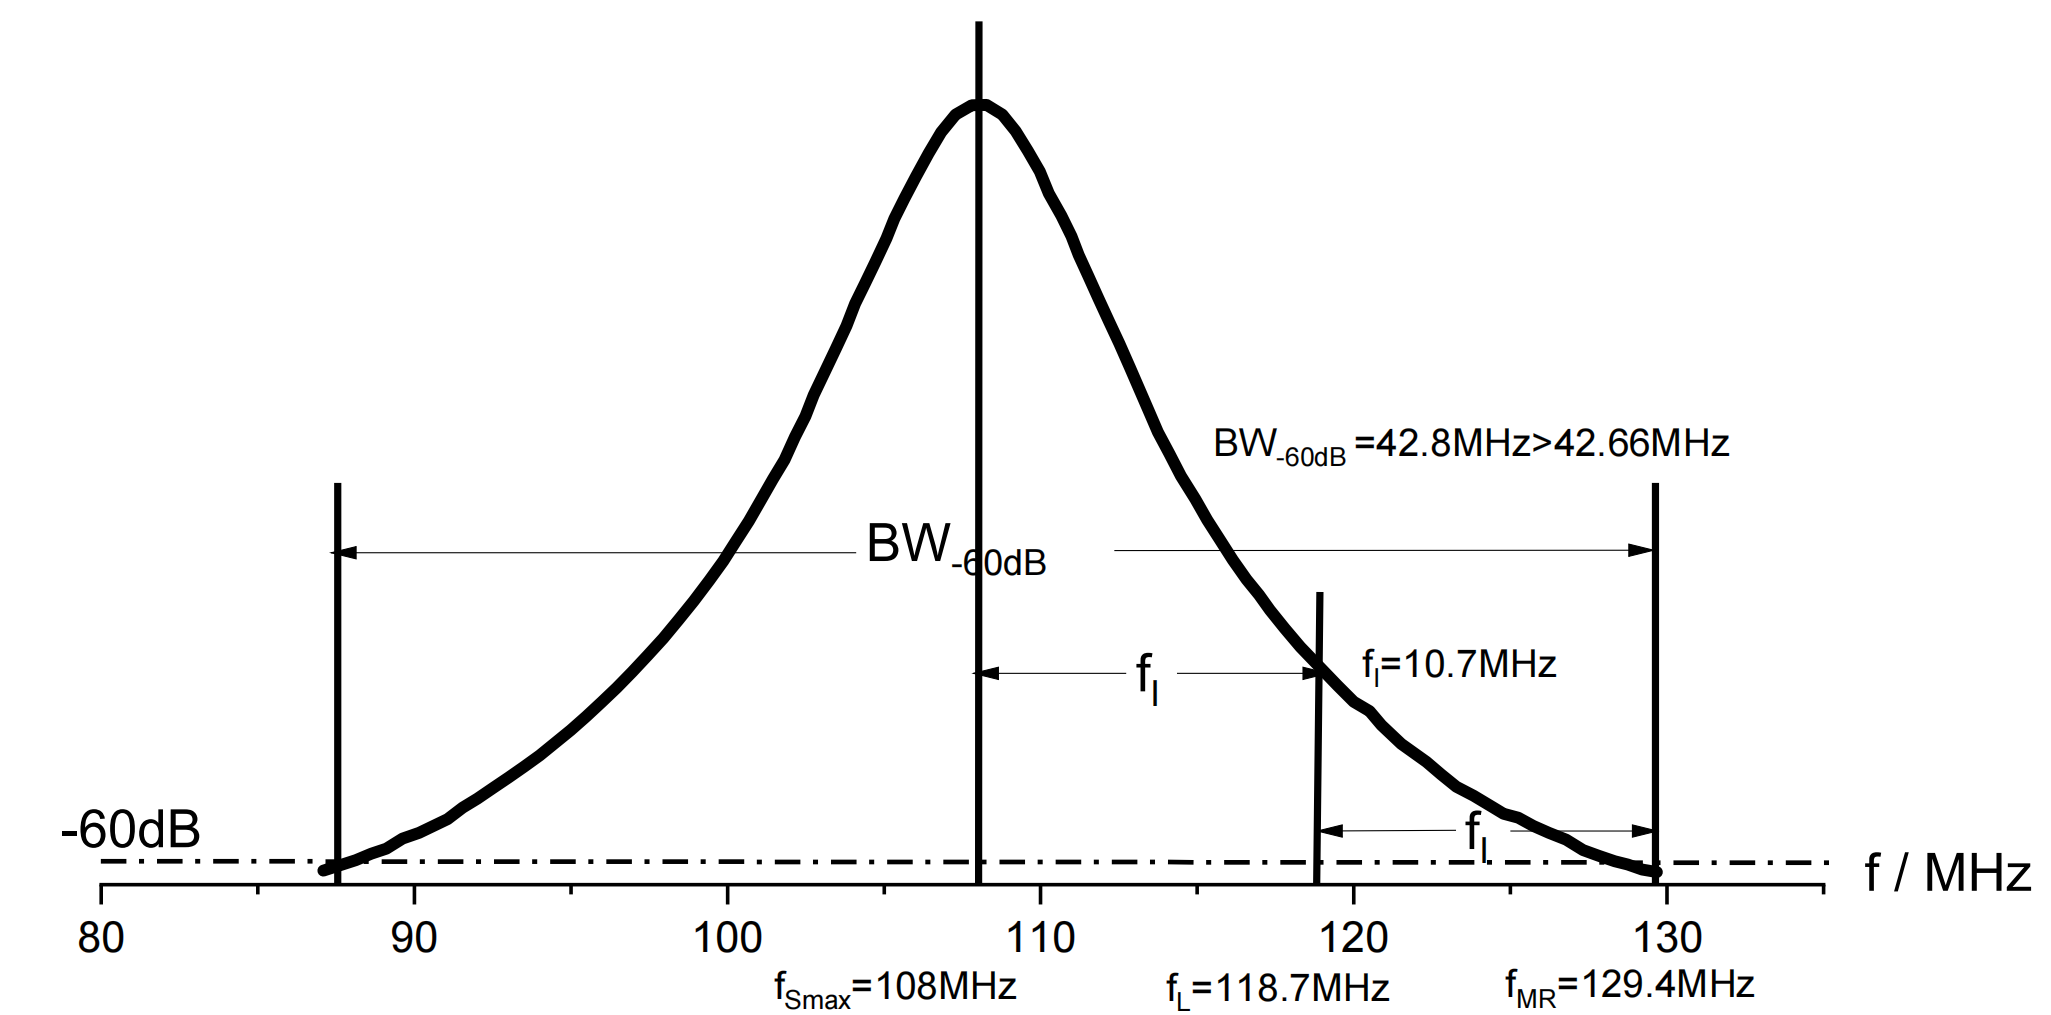
\includegraphics[scale=0.125]{中频选择图形.png}
    \caption{高放级选频特性及中频选择}
    \label{中频选择图形}
\end{figure}


\textbf{[混频电路搭建及参数计算]}

采用单管混频电路设计混频器,如图\ref{混频原理}所示,晶体管基极接高放级输出信号,射极反接本机振荡器输出信号,由于$f_S$与$f_L$从两个端口输入混频器,且谐振在不同频率,因此保证了信号间的隔离度。输入端回路除去直流偏置的总电压$v_{i}$可表示为:$v_{i}=v_{L}+v_S$。

由于混频管需工作在非线性状态,因此基极偏置电压不应过小,直流偏置选用5V时,调节基极偏置电阻$R_{5},R_{6}$,当$R_{5}$工作在10$\mathrm{k}\Omega$,当$R_{6}$工作在20$\mathrm{k}\Omega$,晶体管工作在非线性\footnote{经测试,基极偏置电压为0.5V时无法起到混频作用,即工作在线性状态;基极偏置电压高于0.5V时混频效果明显。}。

对LC并联选频网络,由带宽BW与电感L的关系,可知
\begin{equation}
    BW=\frac{f_0}{Q_L}=\frac{f_0}{\frac{1}{g_L \cdot \rho}}=f_0 \cdot g_L \cdot \omega_0 L
    \label{带宽}
\end{equation}
为了加强混频器谐振网络的频率选择性,应选用较小的电感值,采用$L_4$=1$\mathrm{\mu}$H。

由前述分析,选择中频$f_I=10.7$MHz,则混频器谐振电容$C_{13}=\frac{1}{\omega_0^2\cdot L_4}\approx220$pF。


\begin{figure}[H]
    \centering
    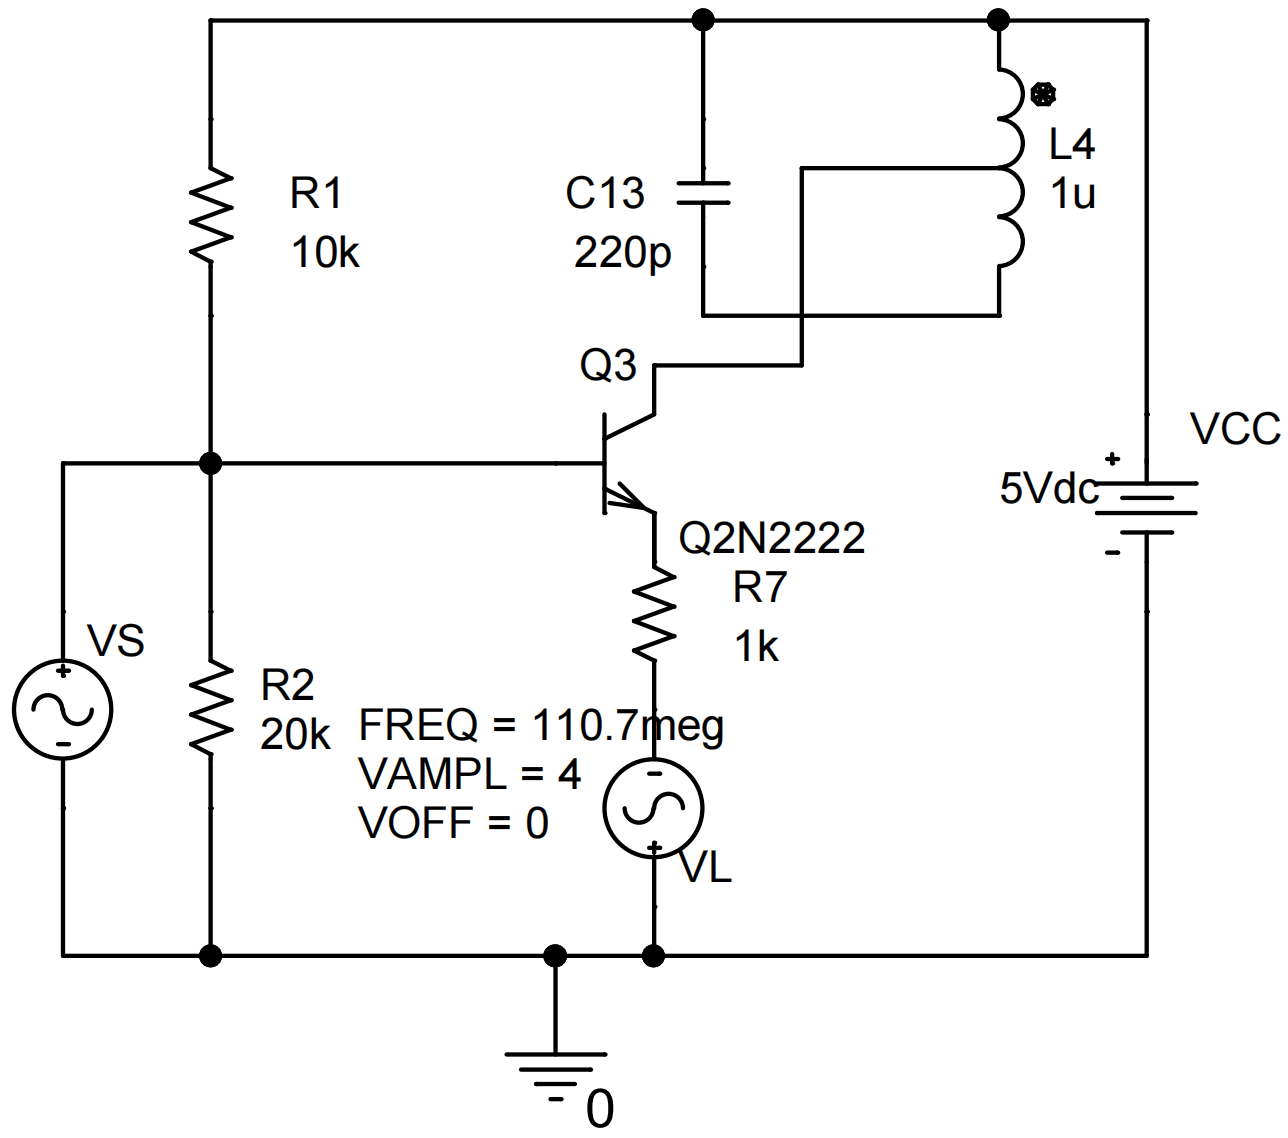
\includegraphics[scale=0.16]{混频电路已调参.png}
    \caption{混频器电原理图}
    \label{混频原理}
\end{figure}
如图\ref{混频原理}所示,电源VS,VL分别代表高放级输出信号与本振输出信号。

可以估算混频器集电极电流在频点上的输出幅度。对集电极电流在基极偏置电压处展开到2阶,有
\begin{equation}
\begin{aligned}
      i_{C}(t)&=\Sigma^{2}_{n=0}a_n\cdot (v_{BE}-V_{BB})^{n}\\
      &= I_{CQ}+g_{m}\cdot v_{i}(t)+\frac{g_m}{2V_T}\cdot v_{i}^2(t)\\
      &=I_{CQ}+g_{m}\cdot (V_{Sm}cos(2\pi f_S t)+V_{Lm}cos(2\pi f_L t))
      \\
      &+\frac{g_m}{2V_T}\cdot {(V_{Sm}cos(2\pi f_S t)+V_{Lm}cos(2\pi f_L t))}^2\\
\end{aligned}
\end{equation}
只考虑频率$f_L-f_S$处的电流成分,由积化和差,得
\begin{equation}
    \begin{aligned}
    i_o(t) = \frac{I_{CQ}}{2\cdot V_T^2}\cdot V_{Sm}V_{Lm}\cdot cos(f_L-f_S)t
    \end{aligned}
    \label{混频跨导}
\end{equation}


\subsection{中放级}
中频放大器用以对10.7MHz中频信号进行放大,为了在后级解调时满足灵敏度要求,增益不能太低,应选用两级中频放大器级联以同时满足功率增益及通频带两项指标。每级放大器之间采用电感耦合,谐振回路负载用以满足阻抗匹配及进一步选频的功能。

\textbf{[功率增益$G_P$与带宽$BW$的估算]}

通过推导式对增益及增益带宽积进行估算,以此设计中频放大器参数。

假设选用晶体管型号Q2N3904,可知其典型参数如下\footnote{参考书目:《高频电路基础(陈光梦)P89》}:
\begin{table}[H]
    \centering
    \begin{tabular}{ccccccccc}
    \toprule[1.2pt]
    \midrule
         晶体管Q2N3904典型参数 & $r_b$ &$r_{\pi}$&$r_{\mu}$&$r_{ce}$&$C_{\pi}$&$C_{\mu}$&$g_{m}$\\
         \midrule
         参数值&10$\Omega$ &3.5k$\Omega$&5M$\Omega$&120k$\Omega$&4.5pF&3.6pF&38mS\\
         \bottomrule[1.2pt]
    \end{tabular}
    \caption{晶体管Q2N3904典型参数}
    \label{tab:my_label}
\end{table}

利用晶体管y参数换算公式,换算出在10.7MHz频率下,对应y参数值如下:
\begin{equation}
\begin{aligned}
    y_{be}&=\frac{1}{r_{\pi}}+\mathrm{j}\omega C_{\pi}=\frac{1}{3.5\times 10^3}+\mathrm{j}\cdot 2\pi \cdot 10.7 \times 10^{6}\cdot 4.5\times 10^{-12}= (0.286+\mathrm{j}0.303) \mathrm{mS}\\
    y_{bc}&=\frac{1}{r_{\mu}}+\mathrm{j}\omega C_{\mu}=\frac{1}{5\times 10^{6}}+\mathrm{j}\cdot 2\pi \cdot 10.7 \times 10^{6}\cdot  3.6\times 10^{-12}=(2\times 10^{-4}+\mathrm{j}0.242) \mathrm{mS}\\
    \Rightarrow 
  y_{ie}&=\frac{y_{be}+y_{bc}}{1+r_b\cdot(y_{be}+y_{bc})}= (0.286+\mathrm{j}\cdot 0.545)\mathrm{mS} \Rightarrow g_{ie}=0.286\mathrm{mS},C_{ie}=51\mathrm{pF}\\
  and\quad y_{oe}&=\frac{1}{r_{ce}}+\frac{1+r_b\cdot (y_{be}+g_m)}{1+r_b\cdot(y_{be}+y_{bc})}\cdot y_{bc}=(38.1+\mathrm{j}\cdot 332)\mathrm{\mu S}\Rightarrow g_{oe}=38.1\mathrm{\mu S},C_{oe}=31\mathrm{pF}\\
  and\quad  y_{fe}&=\frac{g_m-y_{bc}}{1+r_{b}\cdot (y_{be}+y_{bc})}=(37.67-\mathrm{j}\cdot 0.443)\mathrm{mS} \quad\Rightarrow \quad|y_{fe}|\approx 37.67\mathrm{mS}\\
  % y_{re}=&\frac{-y_{bc}}{1+r_{b}\cdot(y_{be}+y_{bc})}\\
\end{aligned}
\end{equation}

设计过程采用第一级中放负载接双调谐回路,第二级中放负载接单调谐回路的设计方式。其中,第一级的双调谐回路采用电感耦合,用以进一步改善混频器输出信号的选择性;第二级单调谐回路在此基础上增加增益单宽积。为了确保有稳定的增益,两级回路电感$L_5,L_7$均设为220$\mathrm{\mu}$H。

两级回路均谐振在10.7MHz中频处,中放电路图如图\ref{中放电原理}所示。
\begin{figure}[H]
    \centering
    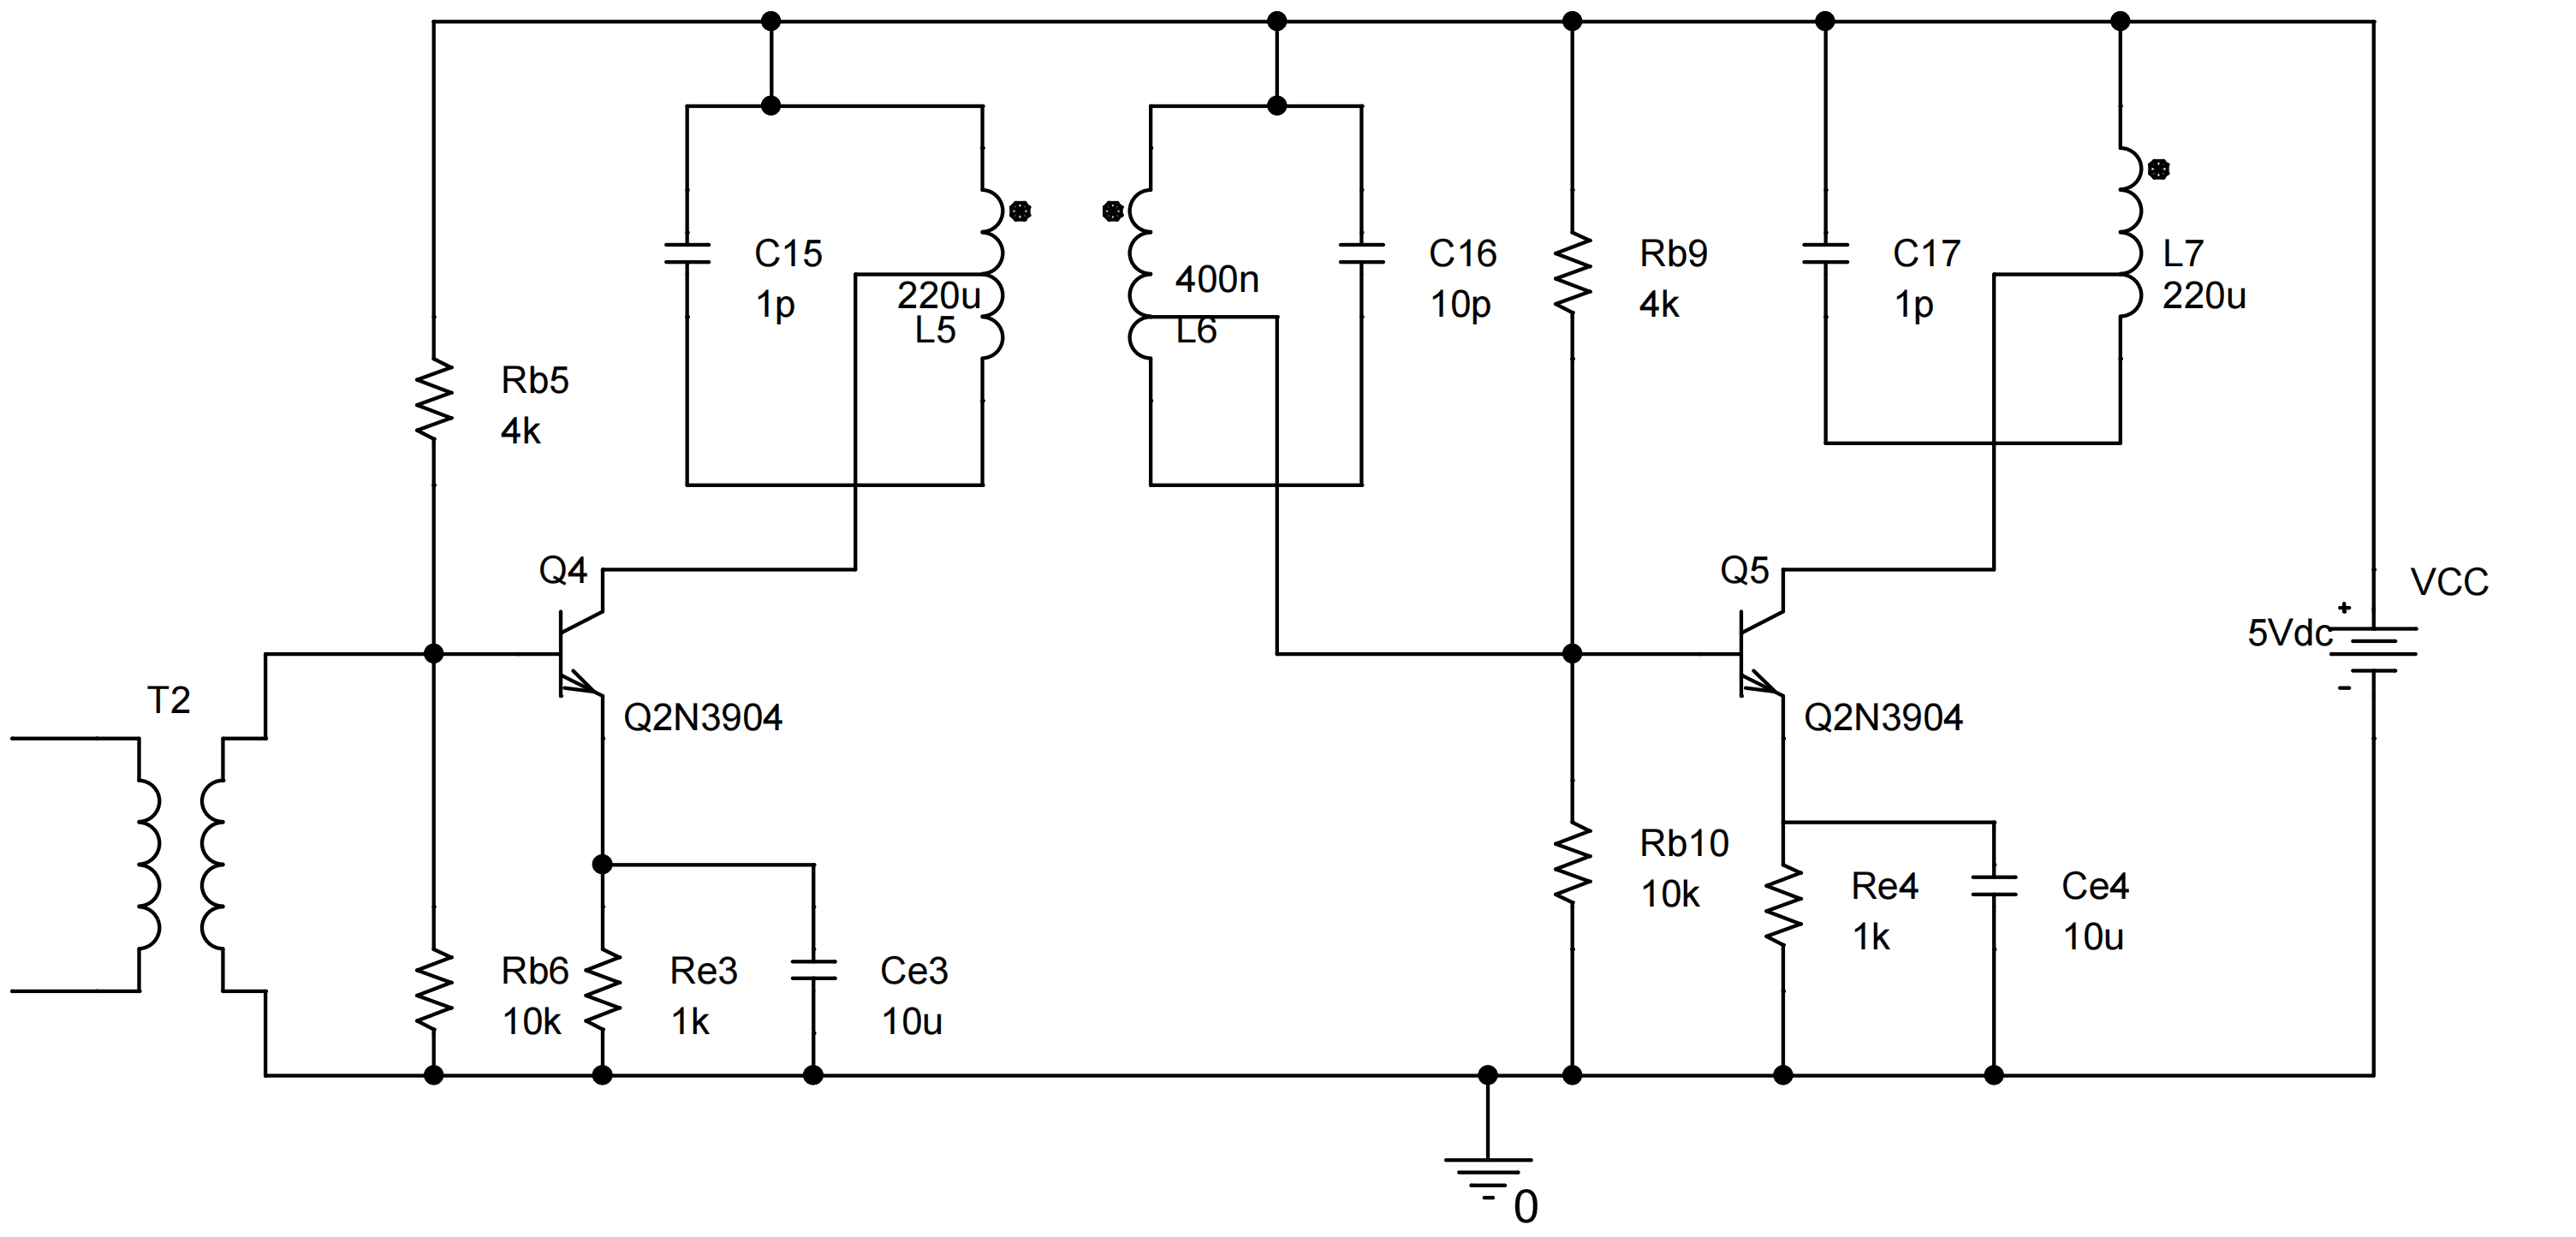
\includegraphics[scale=0.11]{中放电路原理图.png}
    \caption{中频放大器电原理图}
    \label{中放电原理}
\end{figure}

对第一级电感耦合谐振回路,假定在临界耦合状态($\mathrm{\eta}=1$),则增益表达式可写为
\begin{equation}
G_{p1}|_{\mathrm{\eta}=1}=\frac{|y_{fe}|^2}{4g_{ie}g_{oe}}\cdot (1-\frac{Q_L}{Q_0})^2
\label{中放增益式子}
\end{equation}
对第二级单调谐回路,增益$G_{p2}$表达式与\ref{中放增益式子}相同。因此两级中频放大器的总功率增益可以表示为:${G_{p_{\Sigma}}}_{mid}=G_{p1}\cdot G_{p2}$。

对带宽${BW_{\Sigma}}_{mid}$的计算,需要用到归一化的幅频特性。对一级双调谐回路及一级单调谐回路,其总归一化幅频特性可表示为:
\begin{equation}
    {|H(\mathrm{j}\omega)|_{\Sigma}}_{mid}=\frac{2}{\sqrt{4+\xi ^{4}}}\cdot \frac{1}{\sqrt{1+\xi ^2}}
    \label{式18}
\end{equation}
令$ {|H(\mathrm{j}\omega)|_{\Sigma}}_{mid}=\frac{1}{\sqrt{2}}$,则$\xi_{mid}=0.867$。从而带宽${BW_{\Sigma}}_{mid}=\xi_{mid}\cdot \frac{f_0}{Q_L}=0.867\cdot \frac{f_0}{Q_L}$。

由此可见,若采用同种晶体管构成两级中放,则总带宽将变为原先的0.867倍,而增益却变为原先的两倍,起到放大效果的同时又保留了尽可能多的带宽,以此避免音质的损失。

\subsection{解调级}
\begin{itemize}
    \item 解调电路需要考虑灵敏度曲线(S曲线)的鉴频跨导$g_{d}$的大小,根据设计要求,应满足在中频$f_{I}$附近,产生单位频偏df时,$g_{d}\ge 10\mathrm{\mu V}$。
    \item 解调电路的灵敏度曲线需要有足够的线性范围,对调频波带宽$BW_{FM}$里的信号频率,都应处在线性范围之内。
    
    由设计指标,声音带宽为10kHz,假设音频调制基带信号最大频率为F,则F=10kHz。考虑频偏对调频波的影响,由FM调频广播规定,最大频偏$\Delta f_{m}=75$kHz,由Carson公式,估计调频波带宽为:
    \begin{equation}
        BW_{FM}=2\Delta f_{m}+2F=2\times (75k+10k)=170\mathrm{kHz}
        \label{FM带宽}
    \end{equation}
\end{itemize}




\subsubsection{解调电路的选择}
解调的一般过程是将调频波转换为调幅或调相信号,对转化为调幅信号的调频波,采用检波器解调;对转化为调相信号的调频波,采用鉴相器解调。

考虑到频-相变换后解调过程往往需要恒定的10.7MHz信号作为相干解调波,在工程上实现较为困难,且输入信号往往是小信号(如乘积型鉴相器中的模拟乘法器,在输入大信号时无法表现乘性),因此选用调频-调幅转换器(FM-AM)。

振幅鉴频的优点是不需要采用相干解调,可直接通过包络检波的方法从10.7MHz中还原出慢变化信号;另外,基于中频放大器的输出电压往往较大,可利用二极管的单向导通性,对大信号峰值包络检波。

\subsubsection{振幅鉴频电路结构框图}
\begin{figure}[H]
    \centering
        \begin{tikzpicture}
        \node(c)at(-3,0){$v_{FM}$};
        \node(d)at(3,0.4){$v_{FM-AM}$};
        \node(q)at(7,0){$v_{\Omega}$};
        \node [draw,rectangle](a)at(0,0){频率-幅度线性变换};
        \node [draw,rectangle](b)at(5,0){包络检波};
        \draw[->](c)--(a);
        \draw[->](a)--(b);
        \draw[->](b)--(q);
        \label{FM-AM}
        \end{tikzpicture}
    \caption{振幅鉴频电路结构框图}
\end{figure}

\subsubsection{双失谐回路谐振频率选择}
对于频率-幅度线性变换器,采用对称的LC谐振回路作为线性变换电路,使两个LC回路分别谐振在载频($f_{I}=10.7$MHz)的两侧(对于频率分别为$f_{1},f_{2}$),从而两个LC回路幅频特性曲线之差在载频附近即构成S曲线。

实验证明,当频率线性变换范围达到$f_0\pm  0.1\cdot BW_{0.7}$,可以使非线性误差不超过1\%,其对应的最佳LC谐振回路频率值分别为
\begin{equation}
    \begin{aligned}
    f_{1}&=f_{I}+0.62\cdot BW_{0.7}\\
    f_{2}&=f_{I}-0.62\cdot BW_{0.7}\\
    \end{aligned}
    \label{双失谐}
\end{equation}
由设计要求,应满足$(f_0-0.1\cdot BW_{0.7},f_0+0.1\cdot BW_{0.7})\supseteq  (f_0-\frac{BW_{FM}}{2},f_0+\frac{BW_{FM}}{2})$,从而LC回路带宽应满足$BW_{0.7}\ge 0.85$MHz。根据表达式\ref{双失谐},可选择谐振回路频率分别为$f_1=11.2$MHz,$f_2=10.2$MHz。

对LC回路带宽$BW_{0.7}$,由表达式\ref{带宽},在L,C取值确定的情况下,其大小可通过改变总负载电阻的方式调节。
\subsubsection{解调电路}
% 解调电路需要对中放级送出的已调信号进行鉴频,常用的鉴频电路可分为振幅鉴频、相位鉴频、锁相环鉴频等\cite{赵晓阳2016超外差式收音机的调制解调原理},由设计指标:声音带宽10KHz,可知幅频特性曲线


%鉴频跨导即灵敏度;鉴频灵敏度

解调回路电原理图如图\ref{解调电原理}所示,$L_8,C_{18}$构成第一级回路,谐振在频率$f_1$上;$L_9,C_{19}$构成第一级回路,谐振在频率$f_2$上,两级回路负极接在中央。
\begin{figure}[H]
    \centering
    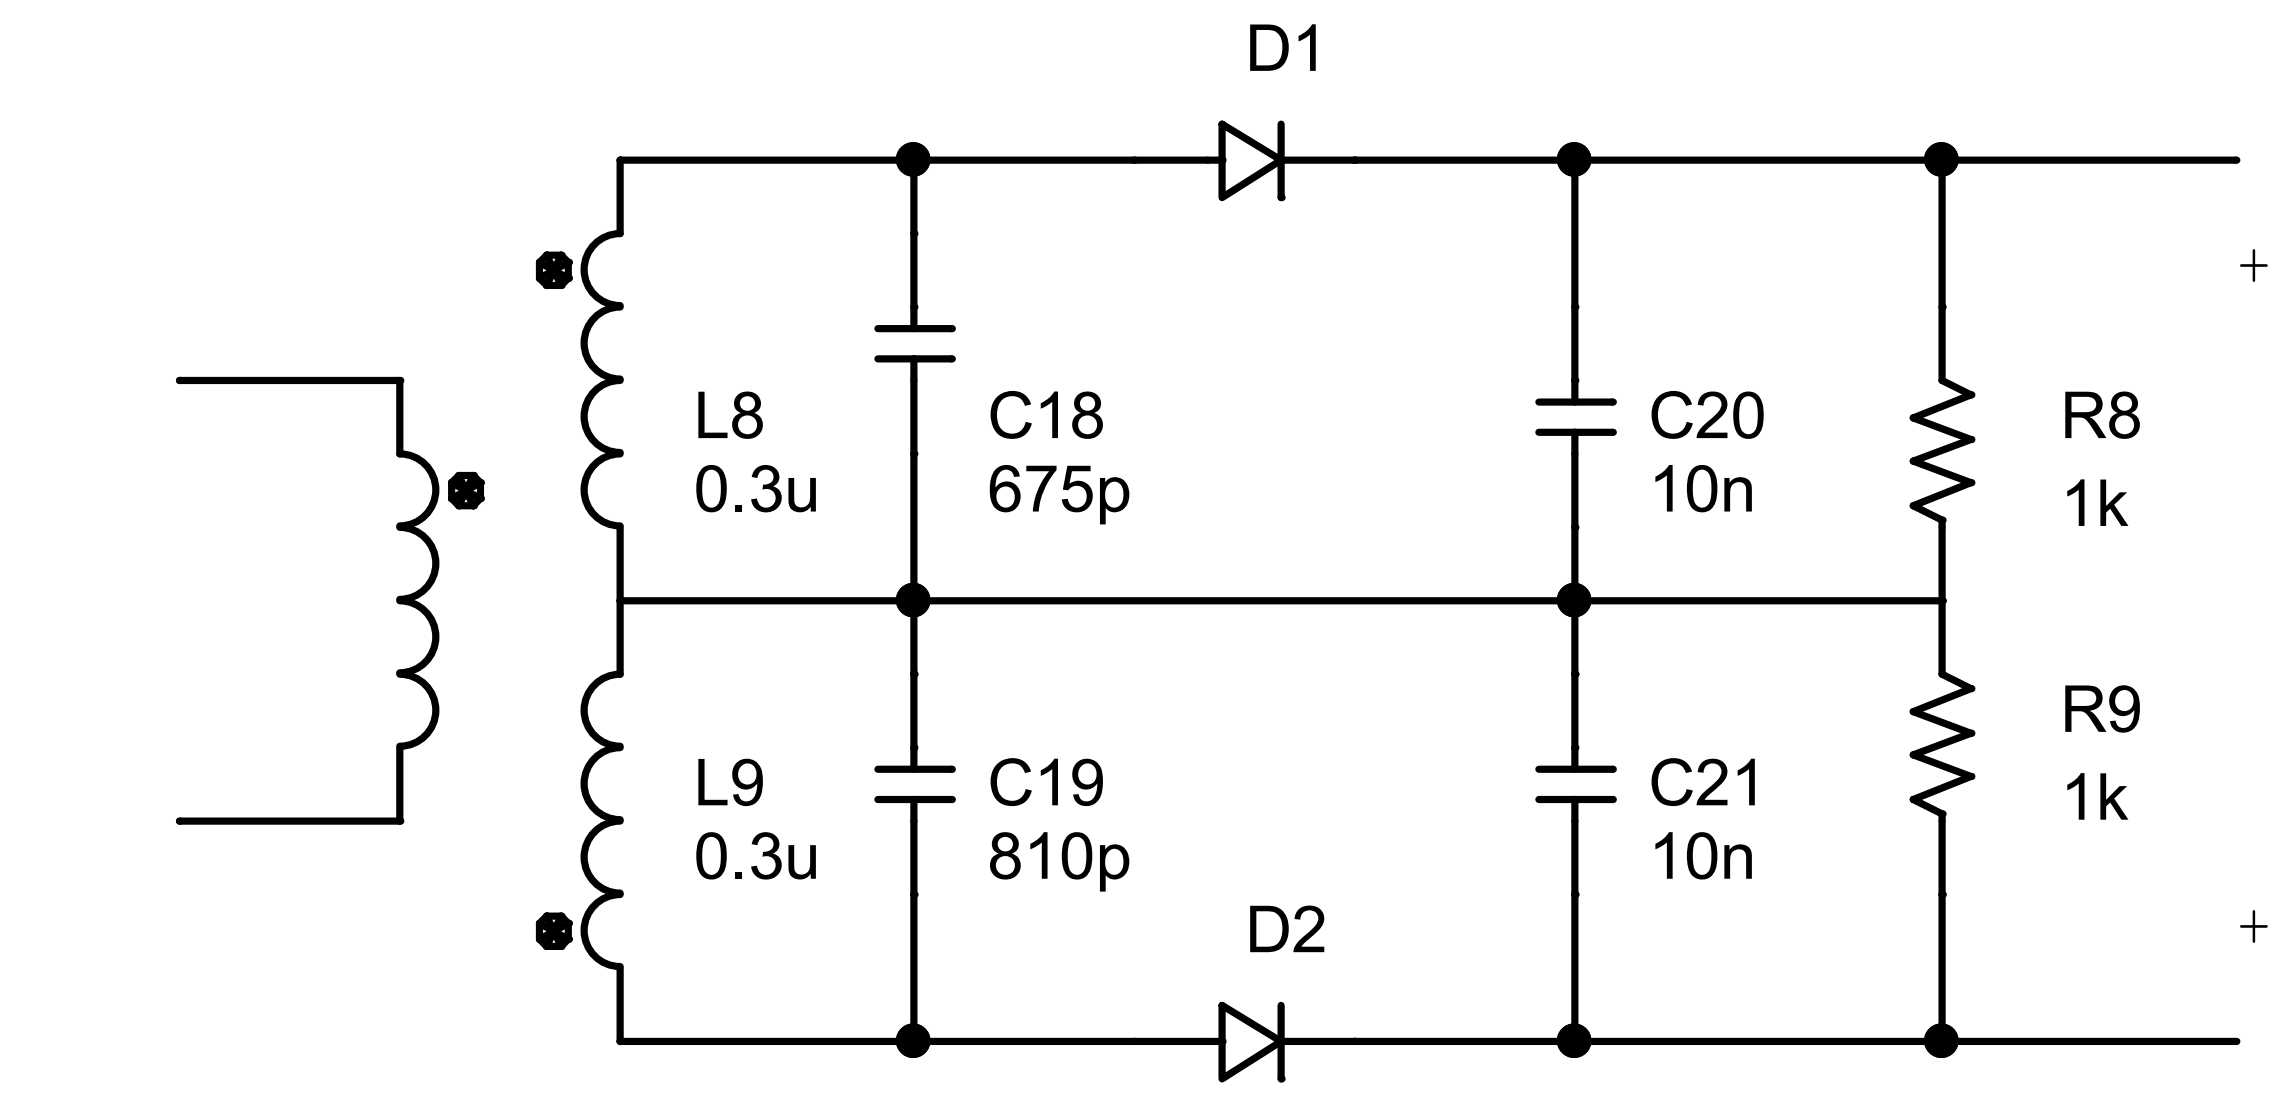
\includegraphics[scale=0.14]{解调电原理图.png}
    \caption{双失谐回路解调电原理图}
    \label{解调电原理}
\end{figure}

二极管$D1,D2$起单向导通作用:输入端电压处在正半周时,上下两个回路对电容$C_{20},C_{21}$充电,当输入端电势低于电容电势,由于二极管的单向导通特性,电容将对RC回路放电,RC常数的大小决定了放电的快慢。

为了检出慢变化信号,RC时间常数应满足
\begin{equation}
    \frac{1}{2\pi F}>RC\gg\frac{1}{2\pi f_{I}}=14.87\mathrm{ns}
    \label{21式}
\end{equation}
取$R_{8}=R_{9}=1\mathrm{k}\Omega,C_{20}=C_{21}=10\mathrm{nF}$,则时间常数$\tau = 10\mathrm{\mu s}$,满足检波要求。




\subsection{低放级}
从鉴频器解调出的音频信号需要通过低频放大以提高音量。由设计要求,声音带宽为10kHz,因此低放级必须有较宽的带宽,以放大解调级输出的不同频率的音频信号。

在负载端,由于扬声器的放音功率往往较大,所以在低频放大器与扬声器之间应接入低频功率放大器,可选用的低频功放如甲类、乙类或甲乙类。但考虑到实际的甲类功放的效率只有约10\%左右,因此采用甲乙类功率放大器作为FM低频功放电路。

低频放大器采用一级NPN管实现前级输入电压的幅度放大,放大后的电压通过由PNP及NPN管构成的乙类放大器(互补输出电路)以放大电流,从而实现功放\cite{谢}。低频级设计电原理图如下所示:
\begin{figure}[H]
    \centering
    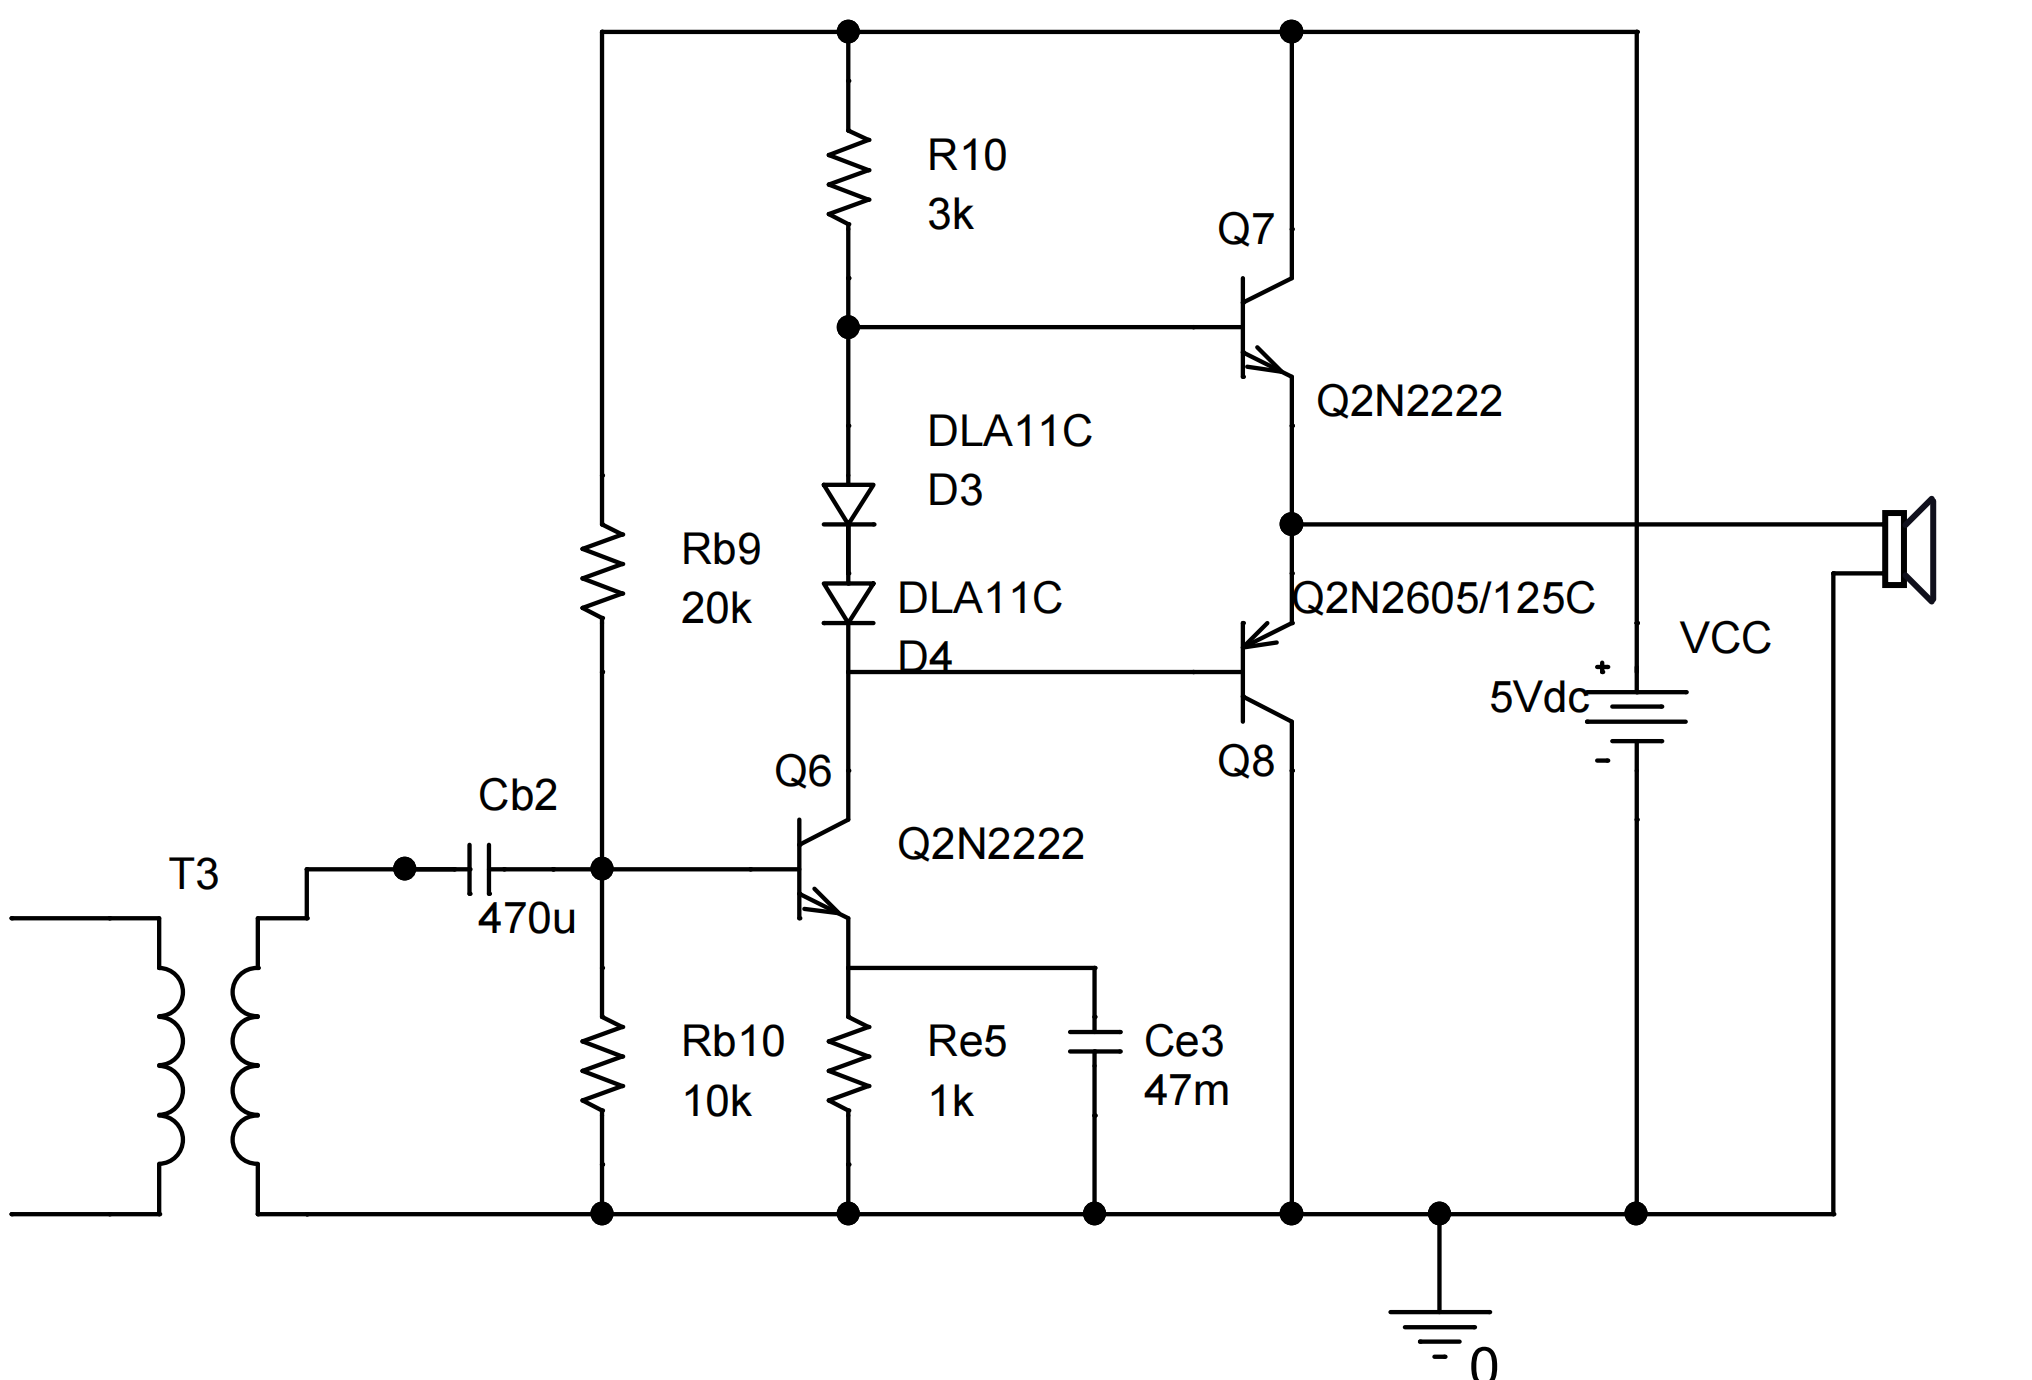
\includegraphics[scale=0.14]{低放sch.png}
    \caption{低频放大器电原理图}
    \label{低放原理图}
\end{figure}

如图\ref{低放原理图}所示,$R_{b9},R_{b10},R_{e5}$起稳定静态工作点作用,旁路电容$C_{e3}$决定了低频放大器的下截止频率$f_L$,由共射放大器下截止频率公式,有
\begin{equation}
    f_{L}=\frac{1+g_m\cdot r_{be}}{2\pi \cdot (r_s+r_{be})\cdot C_E}
    \label{式22}
\end{equation}
由于音频信号往往从0Hz附近开始,所以取较大的旁路电容$C_{e3}=47$mF,以满足带宽要求,使低频声音信号不被衰减。


输出端电压信号$V_{o1}$送至负载,集电极端接电阻$R_{10}$。二极管$D_3,D_4$提供固定压降,使三极管$Q_7,Q_8$处于预导通状态而克服交越失真,当输入信号$V_{o1}>0$,$Q_7$跟随输入,$Q_8$截止;输入信号$V_{o1}<0$,$Q_8$跟随输入,$Q_7$截止。这种互补输出电压$V_{o2}$的方式使电源利用效率得到提升。

对后级功率放大器,其电源利用效率可写为:
\begin{equation}
    \eta = \frac{\pi}{4}\cdot \frac{V_{om}}{V_{CC}}=\frac{\pi}{4}\cdot \frac{V_{CC}-V_{CES}}{VCC}
    \label{效率}
\end{equation}

本设计方案采用$V_{CC}=5V$,远大于极间饱和压降$V_{CES}$,因此低频功率放大器效率可达70\%以上。

\subsection{整机FM收音机电原理图设计}

将上述FM收音机设计各级组合,从而构成完整的收音机模块。在高频与中频各级板块间采用变压器耦合,以达到阻抗匹配的作用,实现信号的最大正向传递过程。

完整FM收音机电原理图如图\ref{横板总电路}所示\footnote{完整、清晰的收音机电路图在附件:“FM收音机设计电原理图.pdf”中给出。}:
\begin{figure}[H]
    \centering
    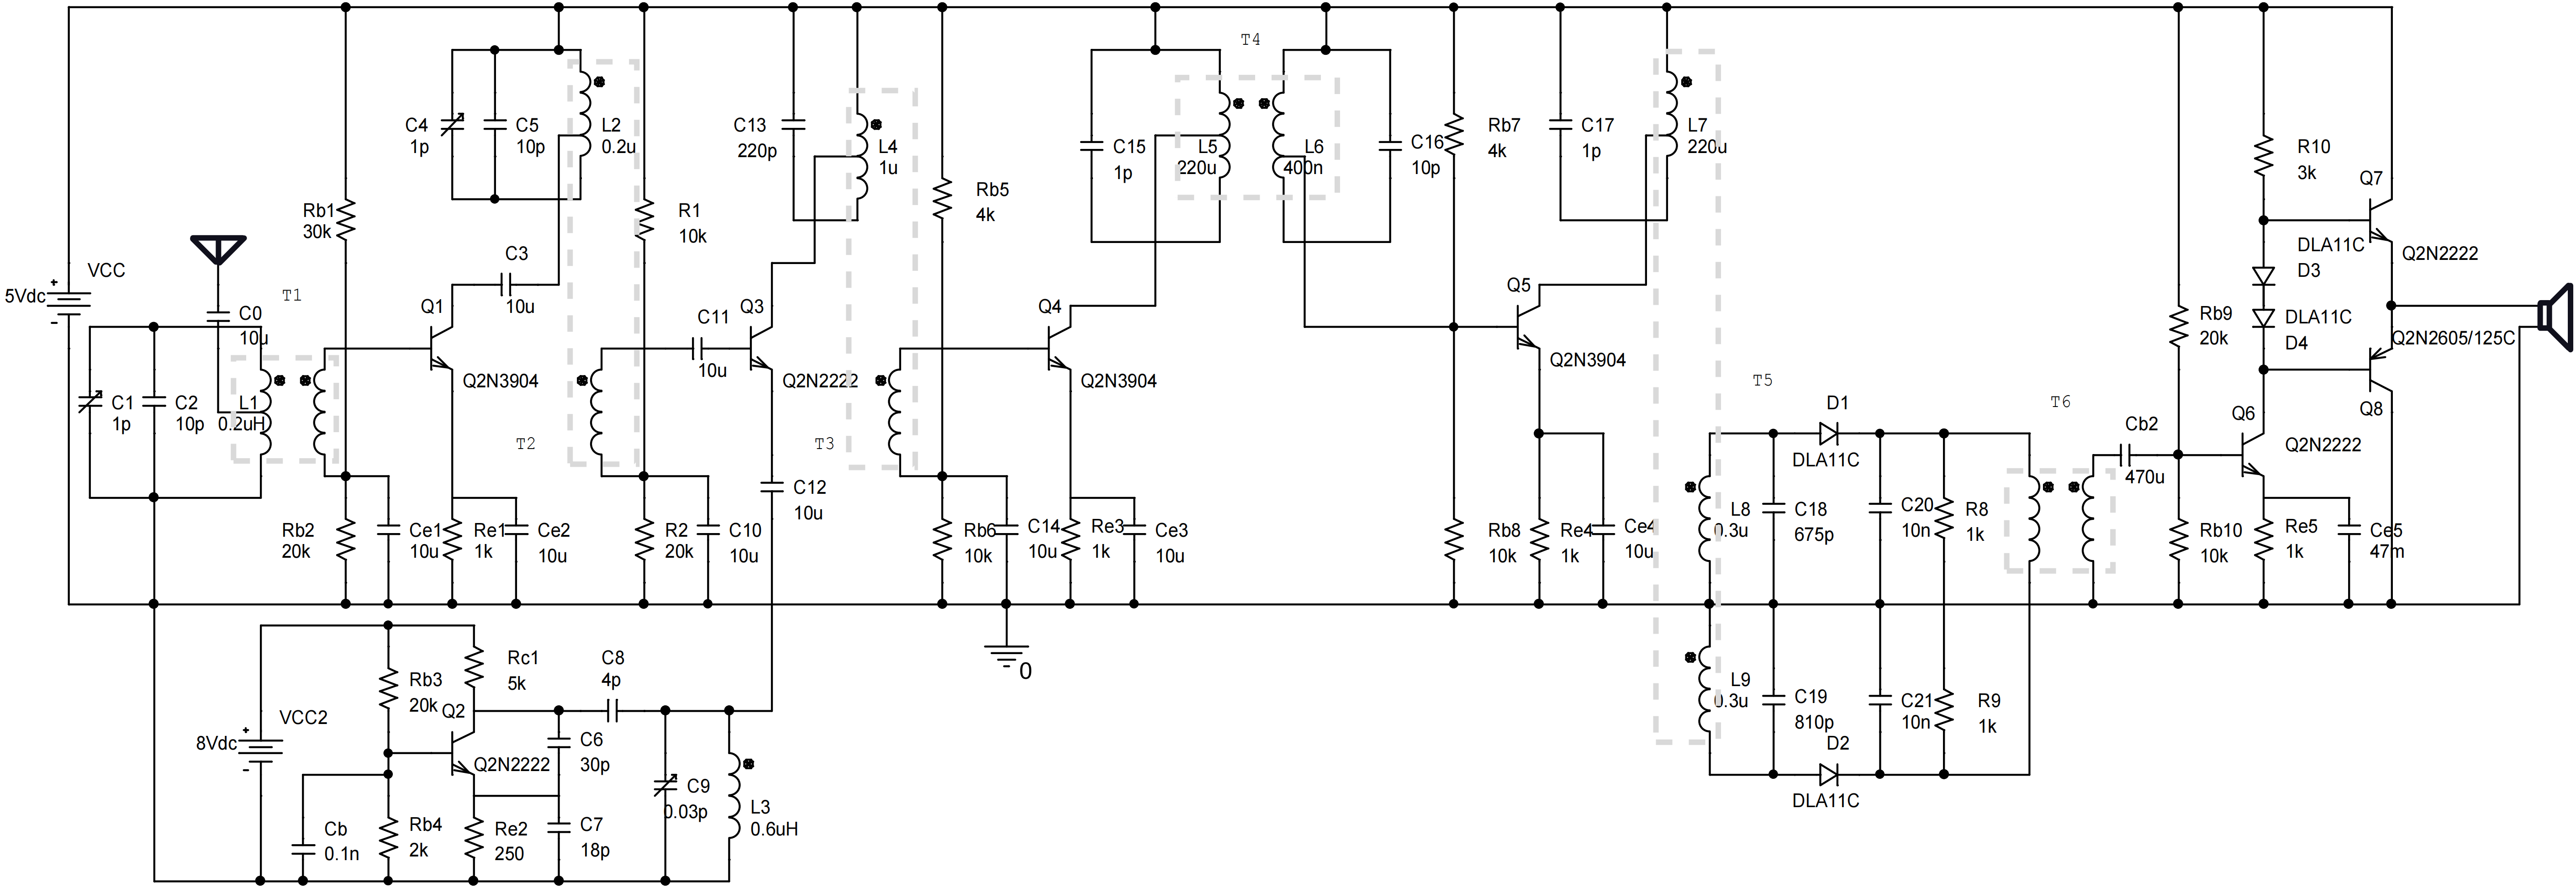
\includegraphics[scale=0.081]{横板总电路图.png}
    \caption{FM收音机总电原理图}
    \label{横板总电路}
\end{figure}


\section{计算机仿真(Pspice OrCAD)}
计算机仿真采用软件Pspice OrCAD模拟,Pspice模拟电路往往具有较好的收敛性,且图形界面友好,可视化程度较高\footnote{模拟仿真电路图按照第二部分的电原理图进行设计,特别地,利用VAC,VSFFM及VSIN三种交流源作为各级输入,利用仿真电感$L_{simu}$替代电原理图中抽头接入部分,采用$K_{linear}$对变压器进行耦合。}。
\subsection{高放级仿真}
高放级仿真包含两部分:时域仿真及频域仿真。对时域仿真,主要考察高频小信号放大器的增益;对频域仿真,主要考察两级调谐回路的选频特性。

\textbf{测试频点}:$f_{c}=107$MHz,\textbf{谐振频点}:107MHz
\subsubsection{高放级时域仿真}
高放级仿真电路包括输入调谐回路与高频小信号放大器两部分,由于天线输入信号为调频波,因此采用FM信号源进行模拟。

FM电压信号源VSFFM含有五个参数,参数名及其含义对照表如下:
\begin{table}[H]
    \centering
    \begin{tabular}{cccccc}
    \toprule[1.2pt]
    \midrule
        VSFFM参数 & VOFF & VAMPL &FC&MOD&FM \\
        \midrule
        参数含义 &直流偏置电压 &交流电压幅值 &载波频率 &调制度 &声音(基带)频率 \\
        \bottomrule[1.2pt]
    \end{tabular}
    \caption{仿真用信号源VSFFM参数对照表}
    \label{VSFFM}
\end{table}

搭根据图\ref{输入头}及图\ref{小信号sch}搭建仿真电路,如图\ref{高放时域仿真sch}所示:
\begin{figure}[H]
    \centering
    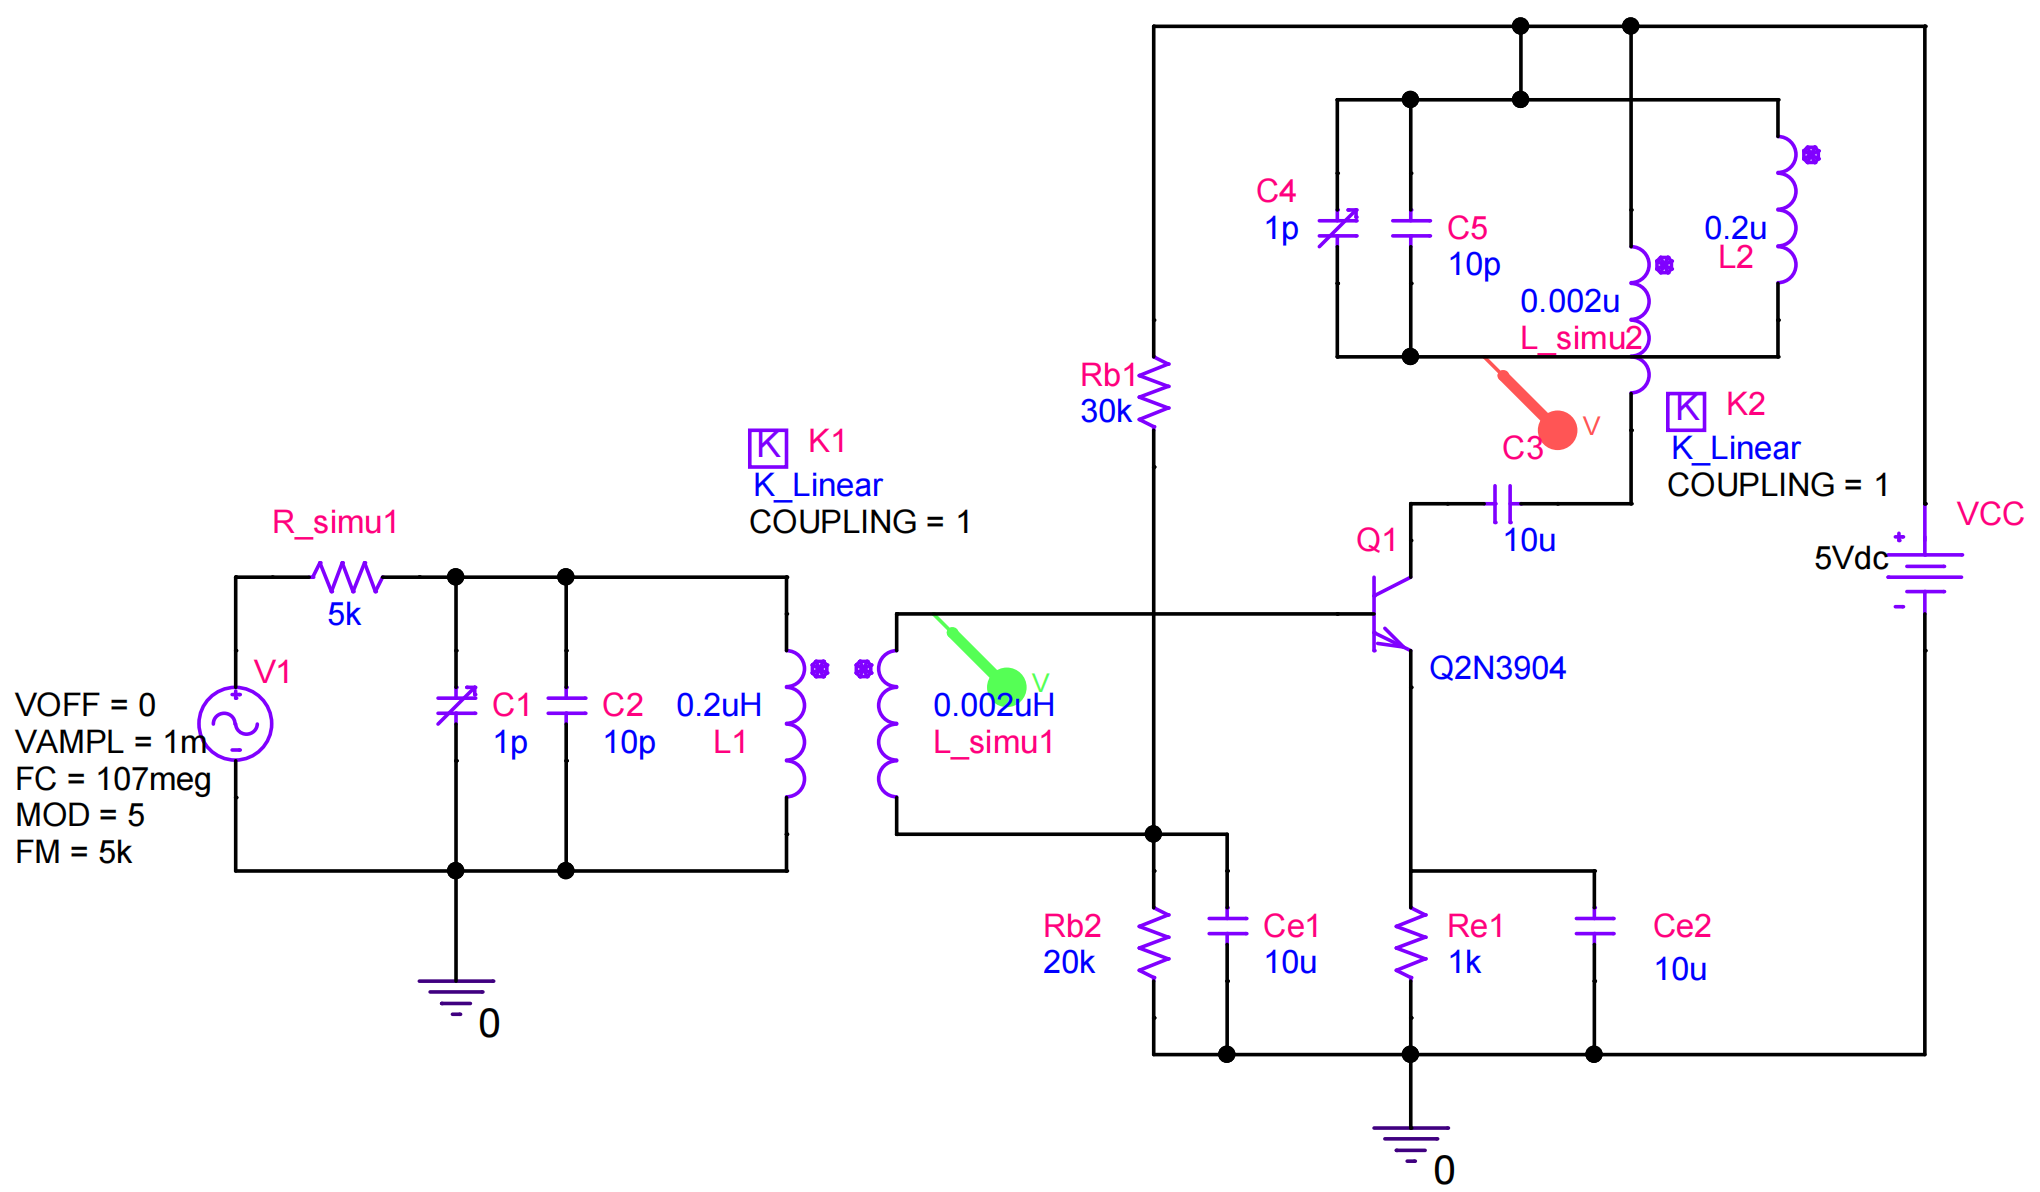
\includegraphics[scale=0.17]{高放级仿真.png}
    \caption{高放级时域仿真电路}
    \label{高放时域仿真sch}
\end{figure}
图中绿表笔接高放级输入端,红表笔接高放级输出端。K1,K2分别代表两级电感耦合(耦合系数设为1),其中电感$L1$与$L\_simu1$耦合,电感$L2$与$L\_simu2$耦合\footnote{原理图中电感采用抽头接入的部分均采用上述耦合方式进行仿真。}。

输入回路端采用幅值1mV的FM电压源进行仿真,得到高放输入端及输出端电压时域波形如下所示:
\begin{figure}[H]
    \centering
    \subfigure[subfigure 1-1][高放输入端]{
        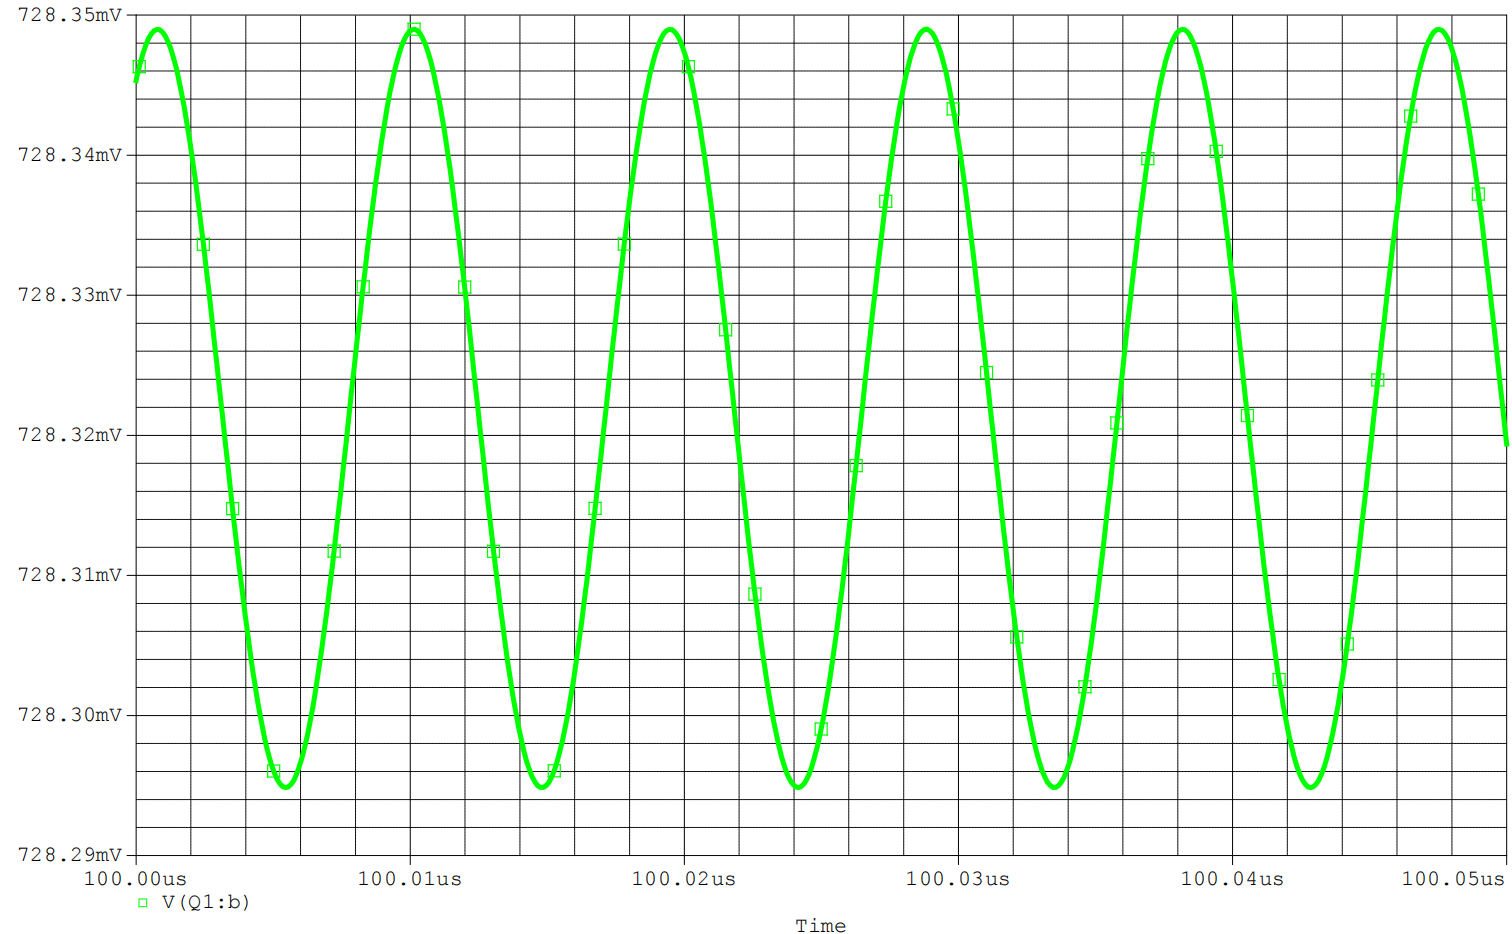
\includegraphics[width=0.4\textwidth]{高放时域波形1.png}
    }
     \hspace{0.01\linewidth}
      \subfigure[subfigure 1-2][高放输出端]{
        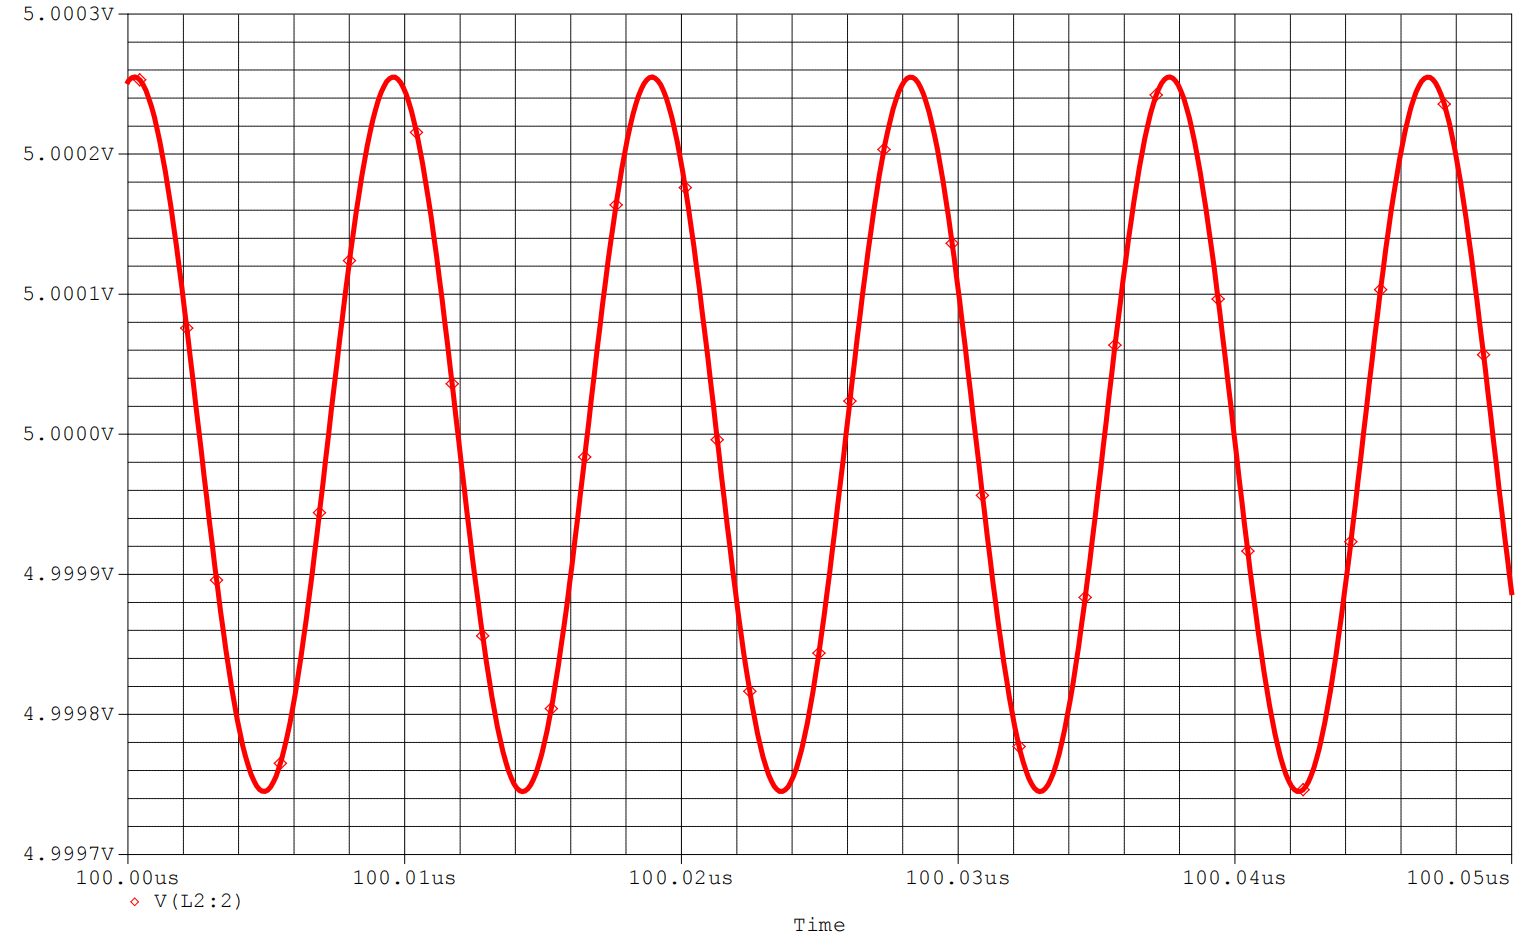
\includegraphics[width=0.395\textwidth]{高放时域仿真2.png}
    }
    \caption{高放级时域仿真}
  \label{高放频域wave}
\end{figure}

计算高频小信号放大器电压增益$G_v$,可得
$$
G_v=\frac{v_{opp}}{v_{ipp}}=\frac{509}{54}=9.426
$$
即能对天线输入信号进行有效放大\footnote{为了使混频级信号工作在线性时变状态以滤除超过2阶的频率合成分量,高放级的输出信号幅度不能过大。}。

\subsubsection{高放级频域仿真}
%%%tiaopingtou.dsn
为了减弱电感耦合时次级阻抗反射到初级的影响,在紧耦合条件下,根据接入系数、匝数比及电感比值的关系,有:
\begin{equation}
    \frac{L_1}{L_2}=(\frac{n_1}{n_2})^2=\frac{1}{p^2}
\end{equation}
即通过调小$L_{simu}$的取值,以减小接入系数,保证谐振回路谐振频点不发生明显偏移\cite{杨文娟2020电力电子变压器中高频变压器的设计方法}。仿真中采用$p$=0.1。


将图\ref{高放时域仿真sch}中FM电压信号源替换为AC电压源,采用扫频AC SWEEP测量两个谐振回路的幅频特性曲线,结果如图\ref{高放频域wave}所示:

\begin{figure}[H]
    \centering
    \subfigure[subfigure 1-1][输入调谐回路]{
        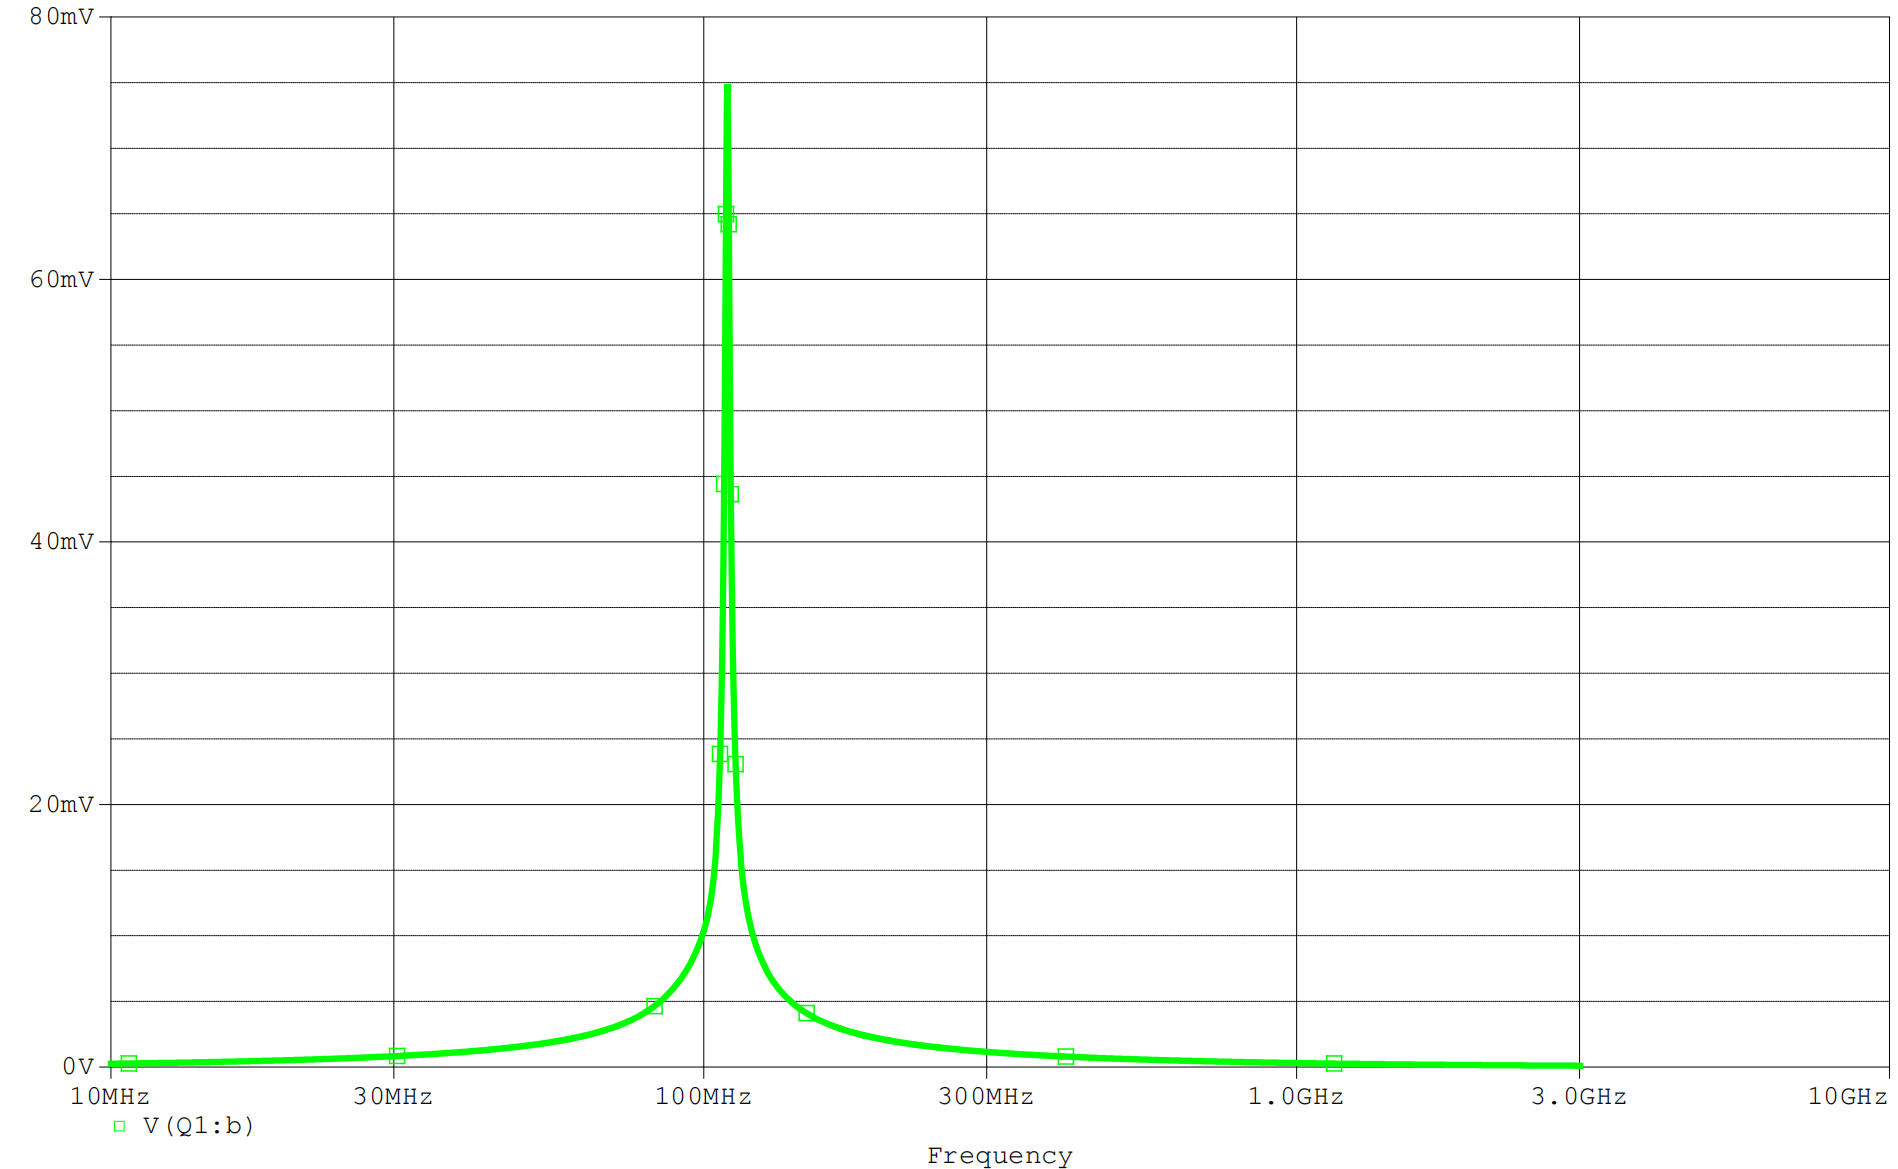
\includegraphics[width=0.43\textwidth]{高放频域1.png}
    }
     \hspace{0.01\linewidth}
      \subfigure[subfigure 1-2][高放调谐回路]{
        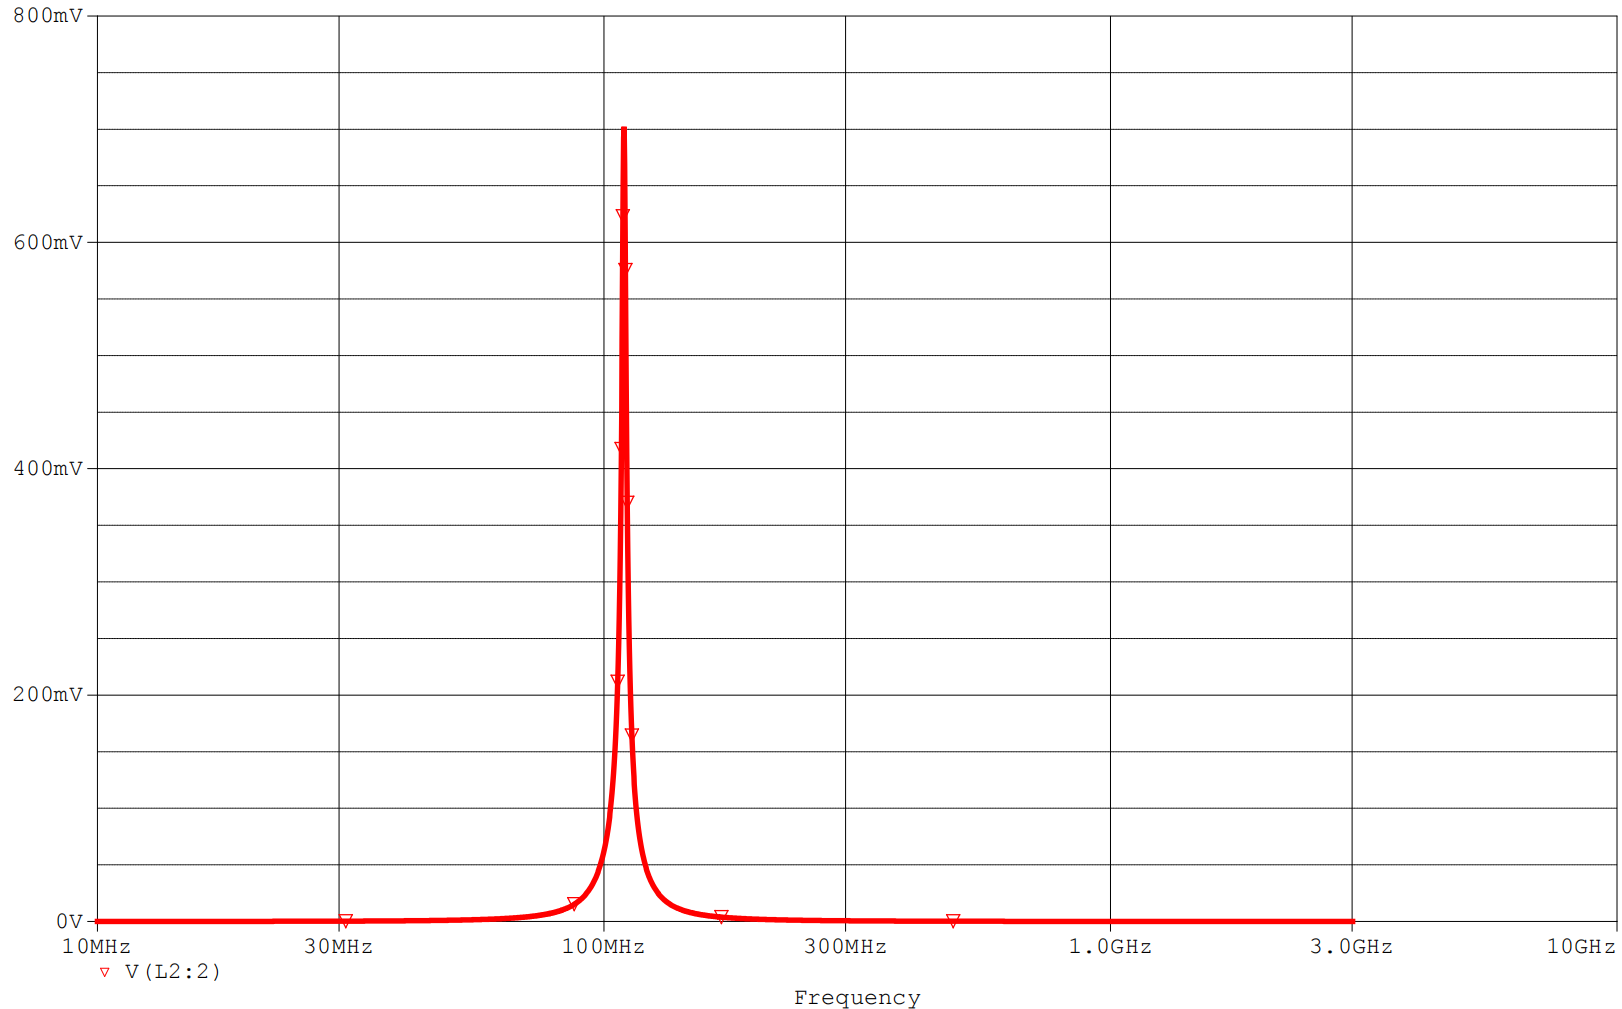
\includegraphics[width=0.42\textwidth]{高放频域2.png}
    }
    \caption{高放级频域仿真}
  \label{高放频域wave}
\end{figure}
通过频域仿真,观察到输入调谐回路与高频小信号放大器调谐回路均谐振在107MHz测试频点上,带宽略高于0.17MHz,能够确保频偏范围内的频率通过,且两级回路组合保障了选择性。

\subsection{本机振荡电路时域仿真}
%%%benzhen_simu.dsn
对本机振荡器频率进行时域测试,对图\ref{本振参数}进行仿真,绿色表笔指向谐振回路输出端,如图\ref{本振仿真电路}。
\begin{figure}[H]
    \centering
    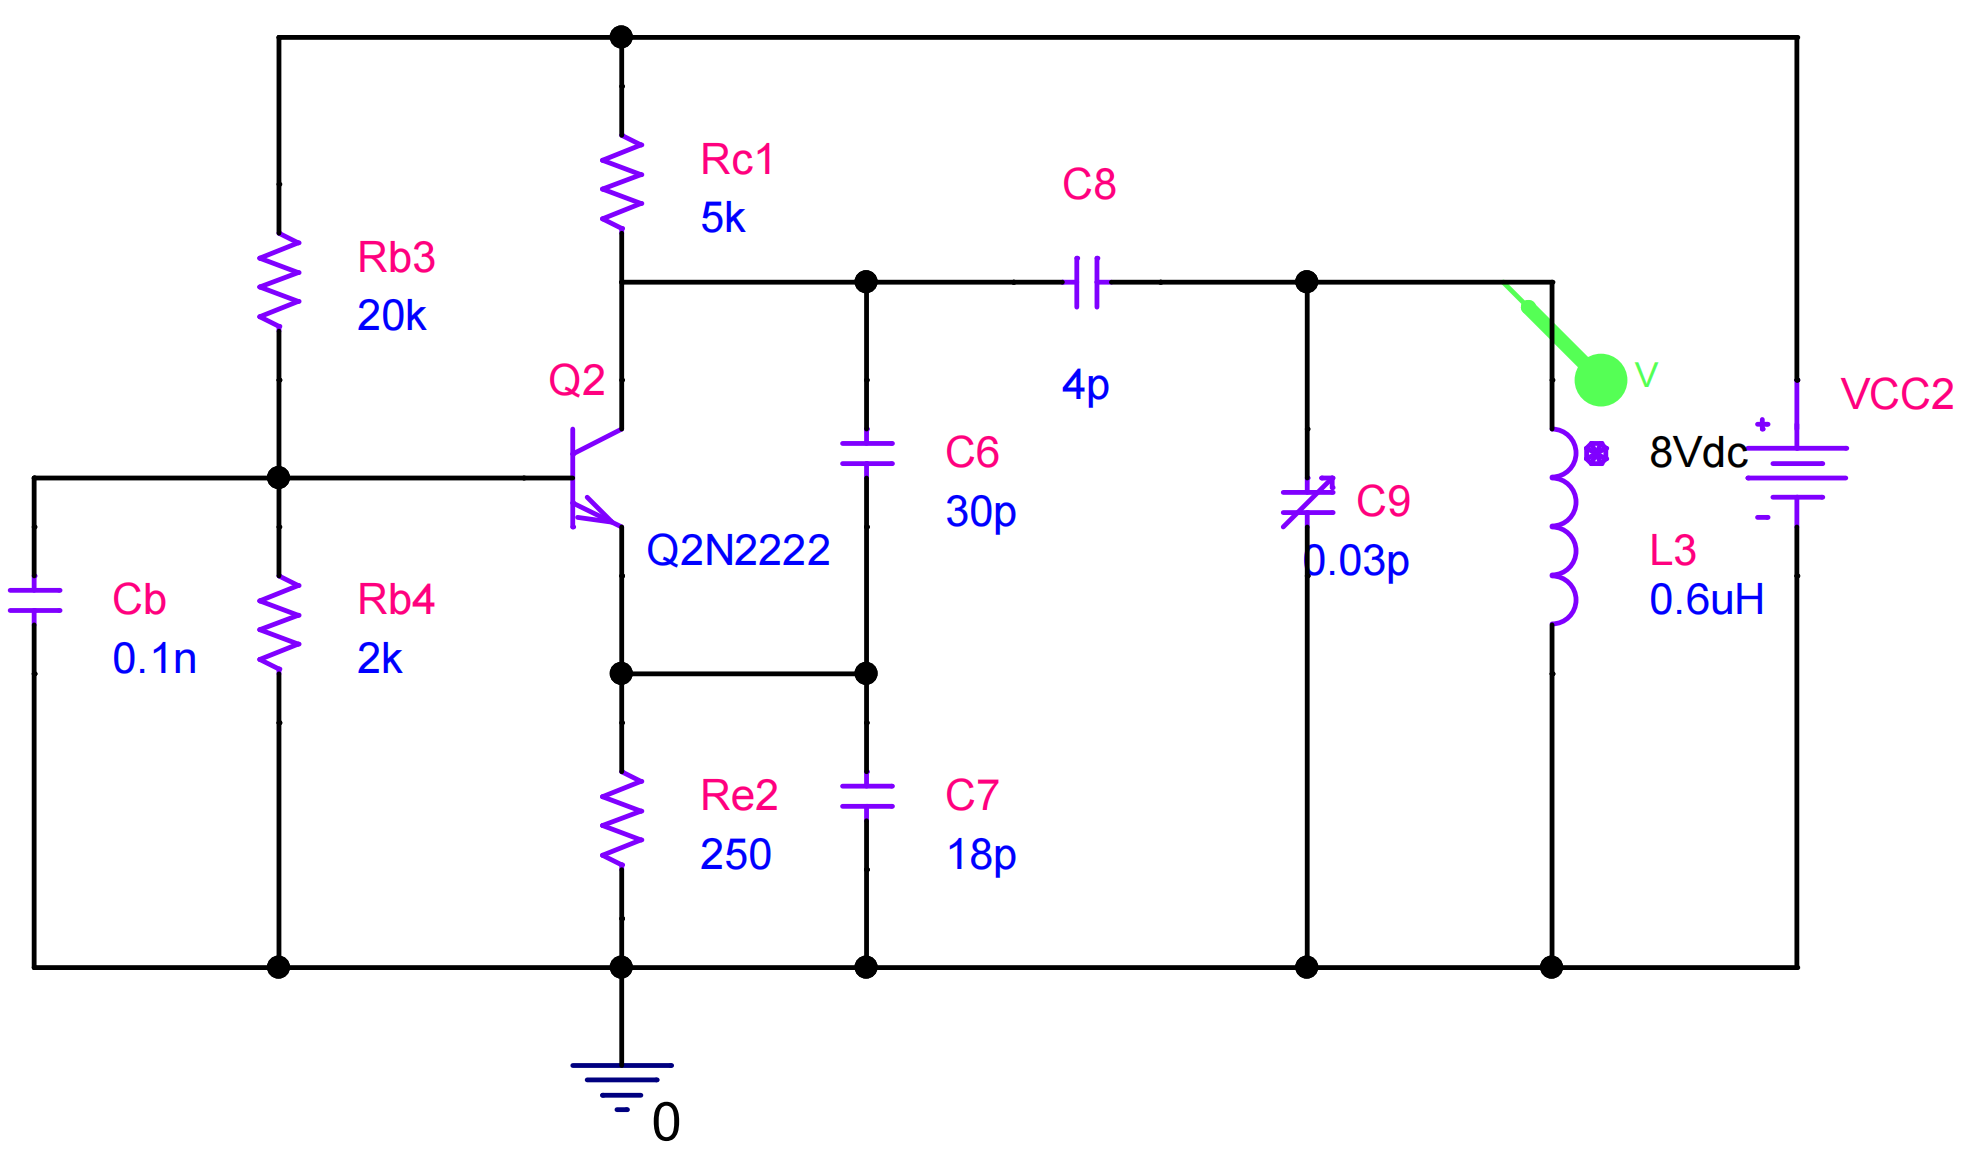
\includegraphics[scale=0.16]{本振仿真电路.png}
    \caption{本机振荡器仿真电路}
    \label{本振仿真电路}
\end{figure}

\textbf{测试频点}:119MHz;\textbf{谐振频点}:119MHz

结果如图\ref{本振_wave}所示。子图(a)中仿真时间跨度为100ns,测量得波形周期为8.41ns,对应本机谐振频率118.9MHz,波峰与波谷无明显波动,即不存在高频寄生振荡;子图(b)中仿真时间跨度从0ns开始至$2\times 10^4$ns结束,期间有超过2000个正弦波,可以看出波形幅度基本稳定,不存在低频寄生振荡和间歇振荡现象。
\begin{figure}[H]
    \centering
    \subfigure[subfigure 1-1][时间跨度$20\mu s-20.1\mu s$]{
        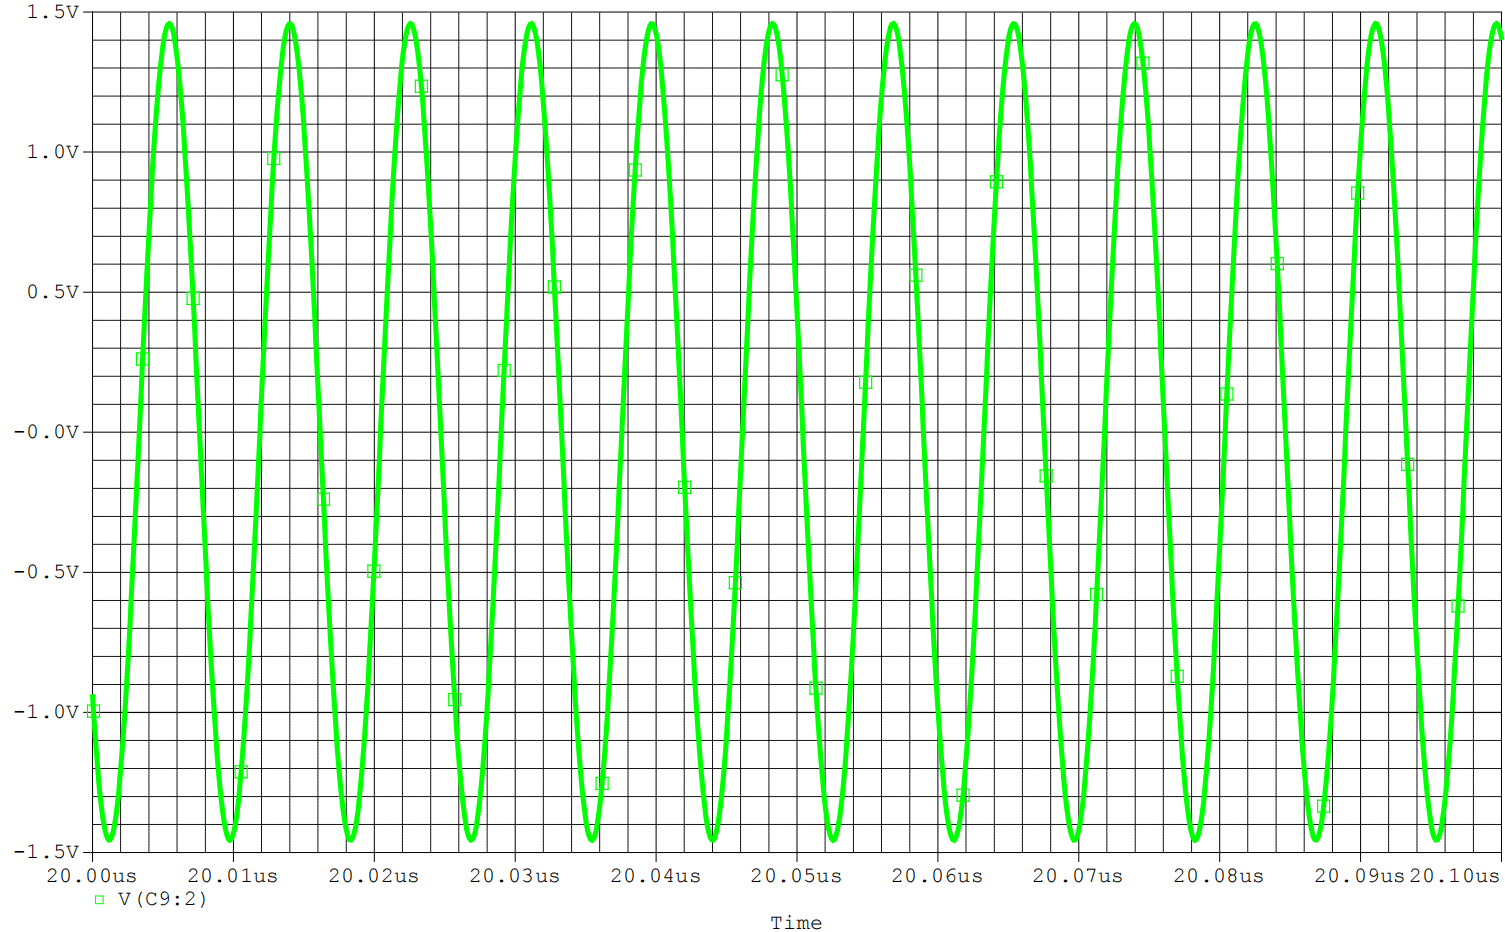
\includegraphics[width=0.43\textwidth]{本振仿真波形1.png}
    }
     \hspace{0.01\linewidth}
      \subfigure[subfigure 1-2][时间跨度$0\mu s-20\mu s$]{
        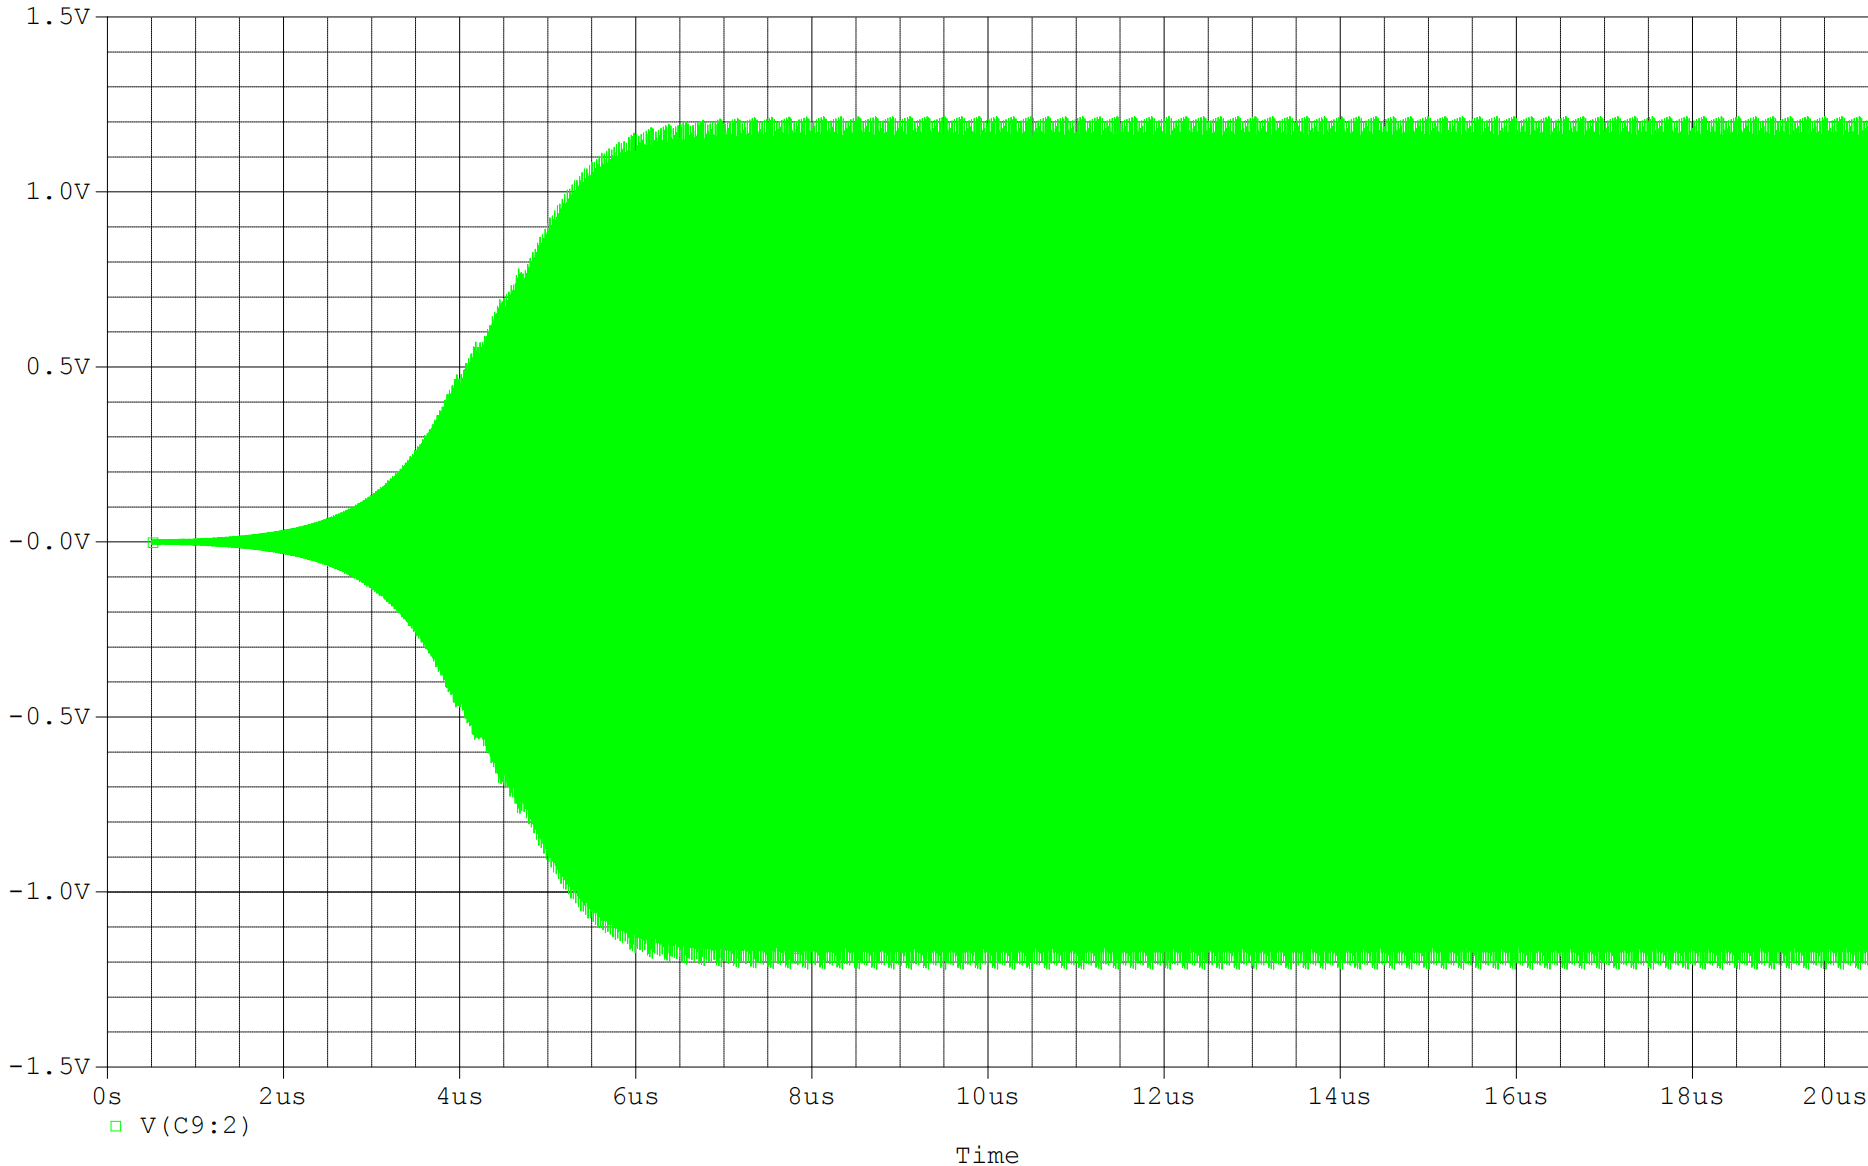
\includegraphics[width=0.43\textwidth]{本振仿真波形2.png}
    }
    \caption{本机振荡电路时域仿真}
  \label{本振_wave}
\end{figure}

由频率准确度计算式,可得本机振荡器频率准确度如下式
\begin{equation}
    \frac{\Delta f}{f_L}=\frac{\hat{f}-f_L}{f_L}=\frac{|119-118.9|}{119}\approx 8.4\times 10^{-4}
\end{equation}
因此振荡器性能较好。



\subsection{混频电路时域仿真}
对混频器进行时域测试,对图\ref{混频原理}进行仿真,蓝色表笔指向晶体管负载的谐振回路,如图\ref{混频仿真电路}。
\begin{figure}[H]
    \centering
    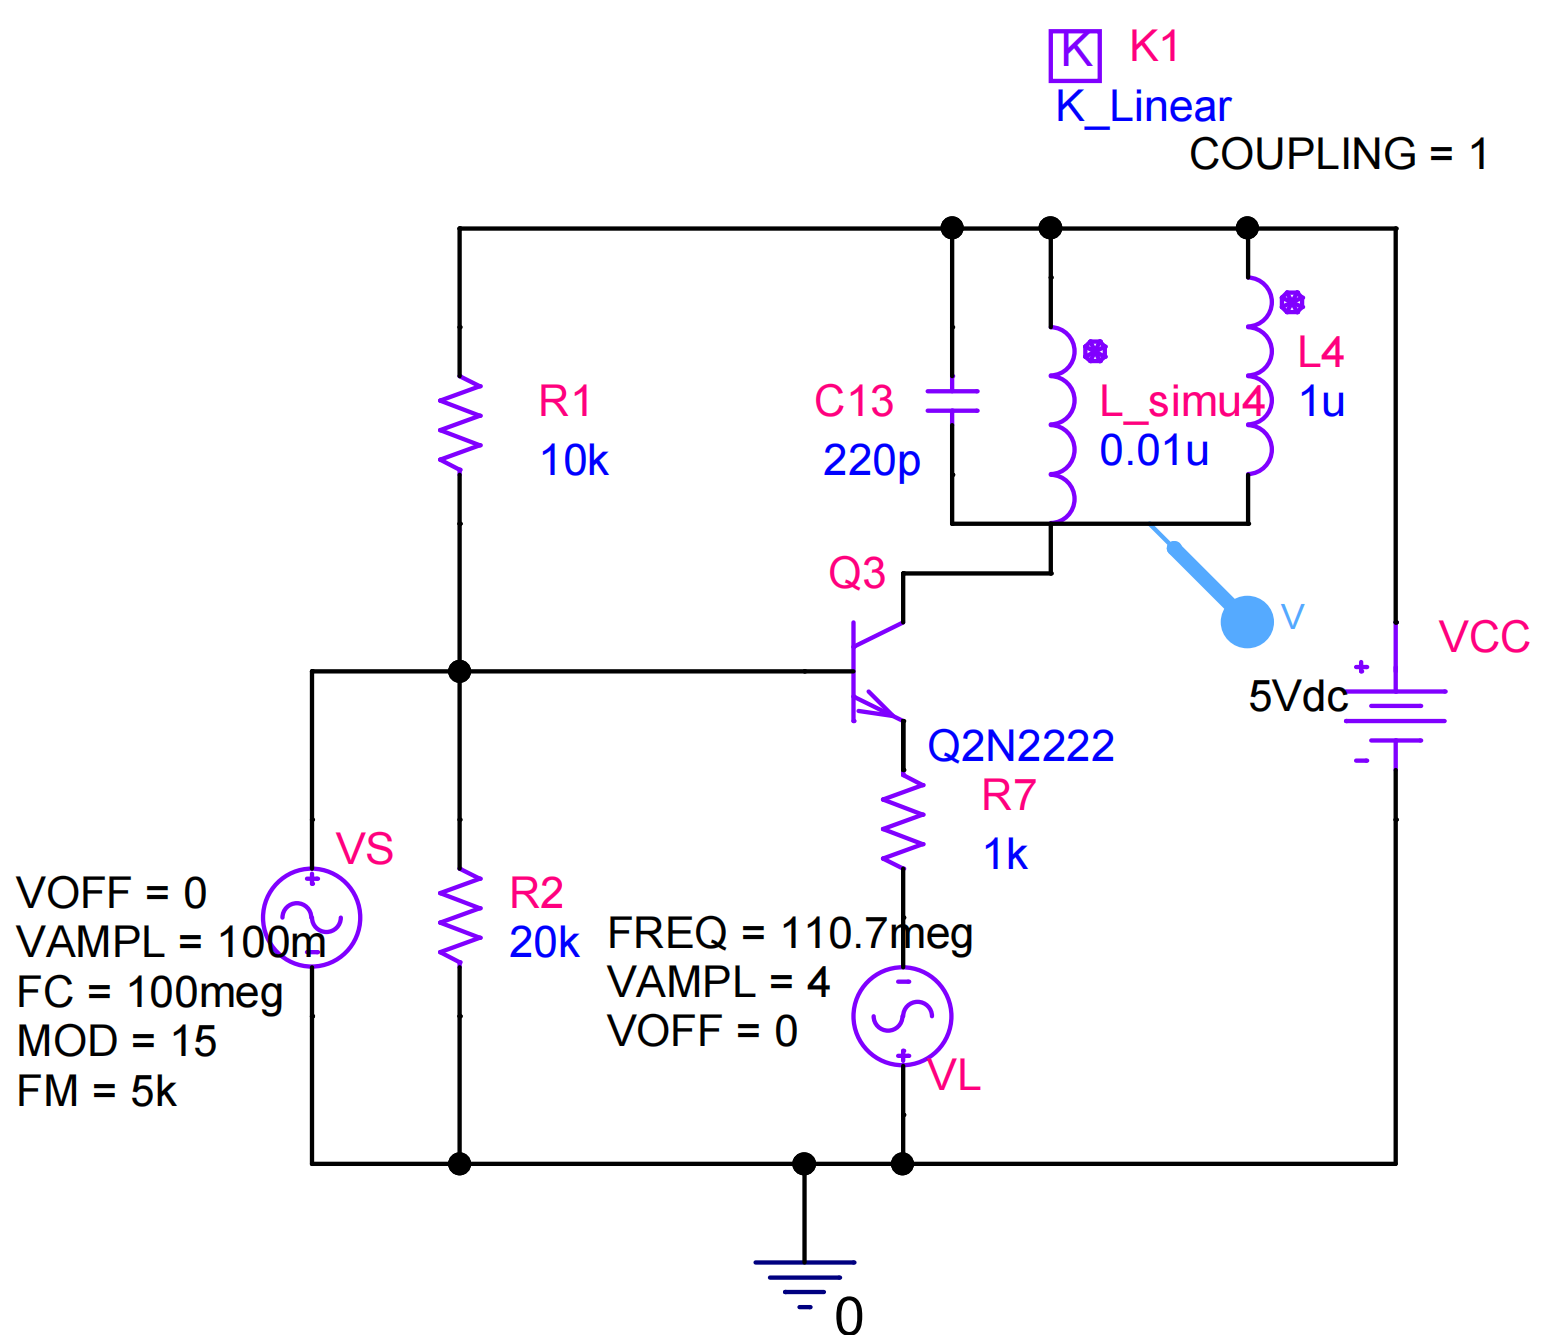
\includegraphics[scale=0.18]{混频仿真电路.png}
    \caption{混频器仿真电路}
    \label{混频仿真电路}
\end{figure}

\textbf{测试频点}:调频信号$f_S=100$MHz,本机信号$f_L=110.7$MHz;\textbf{谐振频点}:10.7MHz

调频信号设定为小信号,采用100mV交流振幅;本机信号设定为大信号,采用4V交流振幅。通过瞬态分析,在时域2000ns至3000ns对混频器输出波形仿真,结果如图\ref{混频wave}所示:
\begin{figure}[H]
    \centering
    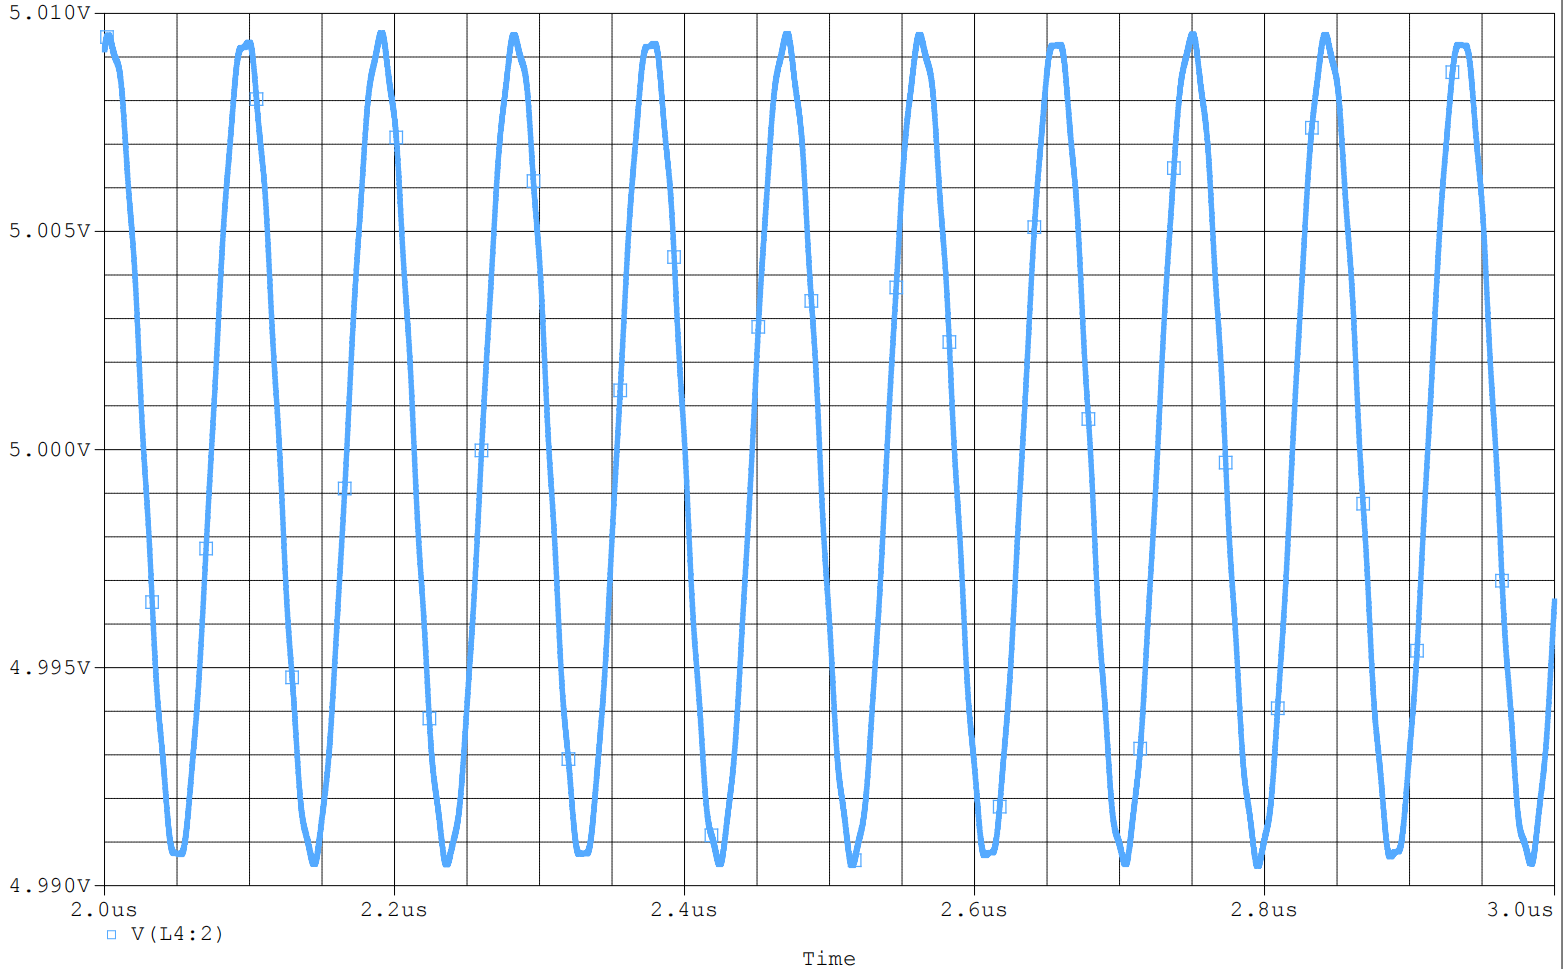
\includegraphics[scale=0.19]{混频时域.png}
    \caption{混频电路时域仿真}
    \label{混频wave}
\end{figure}

利用十字光标测量得到波形相邻间隔93ns,对应频率10.7MHz。观察波峰及波谷,高频信号(110.7MHz及100MHz)幅度被谐振回路滤除,即能够起混频作用。

测量得仿真电路静态工作点电流$I_{CQ}\approx 0.325$mA,由式\ref{混频跨导},得到输出电流$i_{o}(t)$幅值约96mA。

由线性时变电路的混频跨导计算式,得到仿真混频电路的混频跨导$g_C$如下:
\begin{equation}
    g_C\approx \frac{1}{2}g_{mQ}\cdot \frac{V_{L}}{V_T}=\frac{I_{CQ}V_L}{2\cdot V_{T}^2}=\frac{0.325\times 10^{-3}\times 4}{2\times (26\times 10^{-3})^2}=0.96\mathrm{S}
    \label{式26}
\end{equation}


\subsection{中放级仿真}
%%zhongfang_simu.dsn Page1
\textbf{测试频点}:10.7MHz;\textbf{谐振频点}:10.7MHz

中放级仿真包含时域及频域仿真:时域仿真用以对电压放大倍数及电流放大倍数进行测量,以此进一步计算功率增益$G_{p}$,并与额定功率增益计算式结果比较;频域仿真用以测量谐振点是否稳定在10.7MHz。
\subsubsection{中放级时域仿真}
对中放级进行时域仿真,以测试中放级功率增益。分别利用电压表笔(橙)、电流表笔(紫)测量输出谐振回路电压、电流大小,仿真电路如图\ref{中放仿真}所示\footnote{图中K3代表电感$L\_simu5\_1,L5,L6,L\_simu6$互相之间形成耦合关系;K4代表$L_simu7,L7$之间形成耦合关系。}:
\begin{figure}[H]
    \centering
    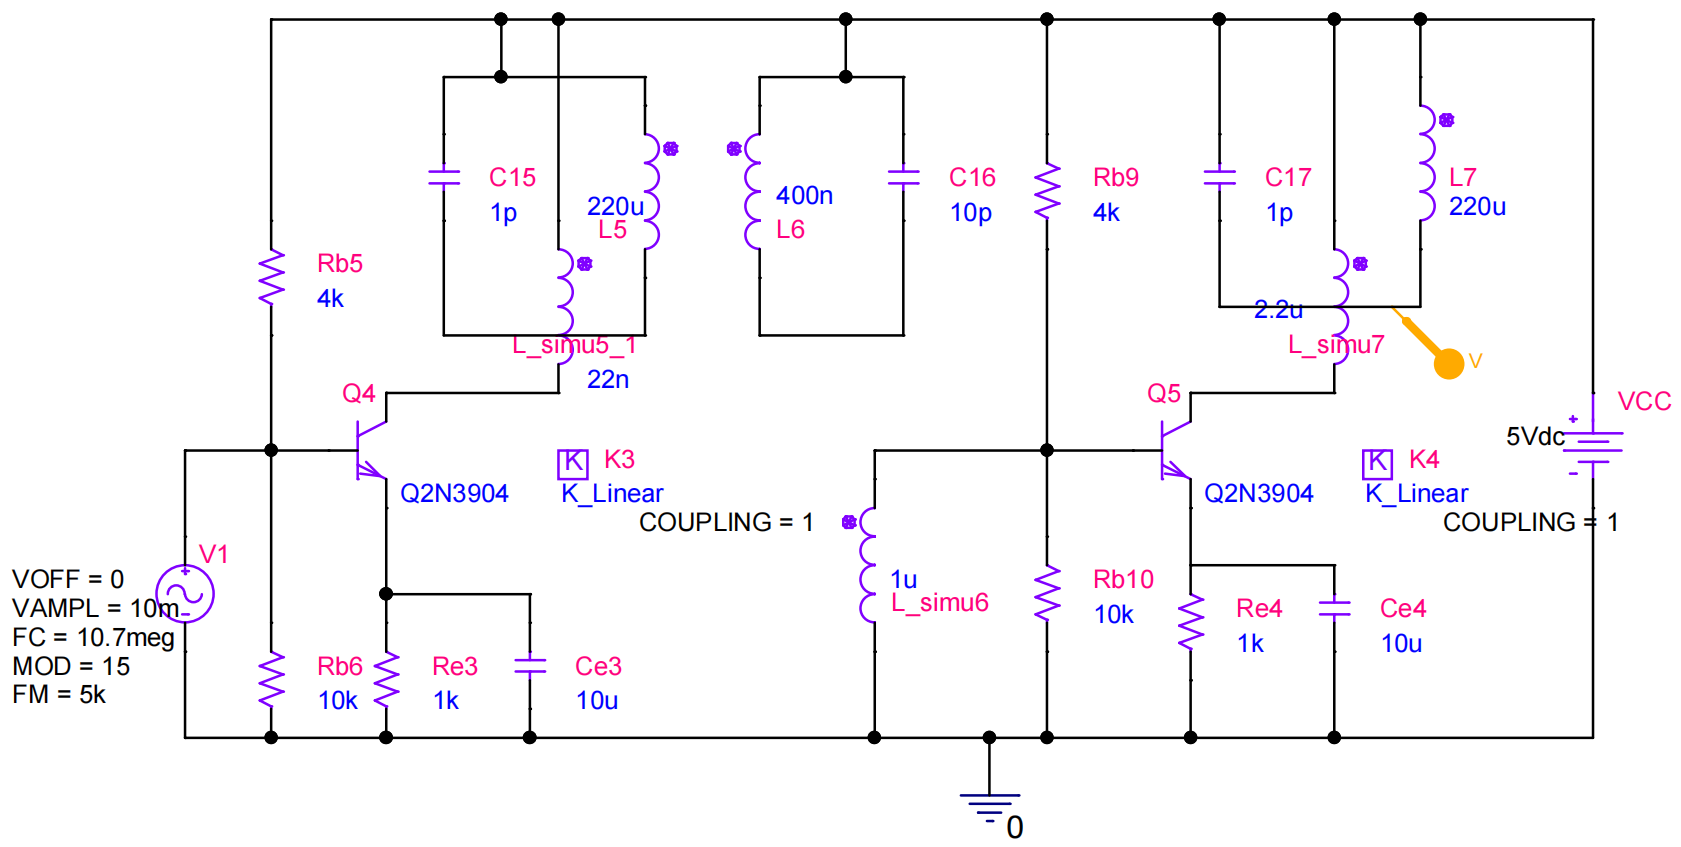
\includegraphics[scale=0.2]{中放仿真.png}
    \caption{中级放大仿真电路}
    \label{中放仿真}
\end{figure}
测量得到波形如下所示,左子图(a)代表输出电压;右子图(b)上侧为输入级电流,下侧为输出级电流。
\begin{figure}[H]
    \centering
    \subfigure[subfigure 1-1][$v_{opp}=$1.133V]{
        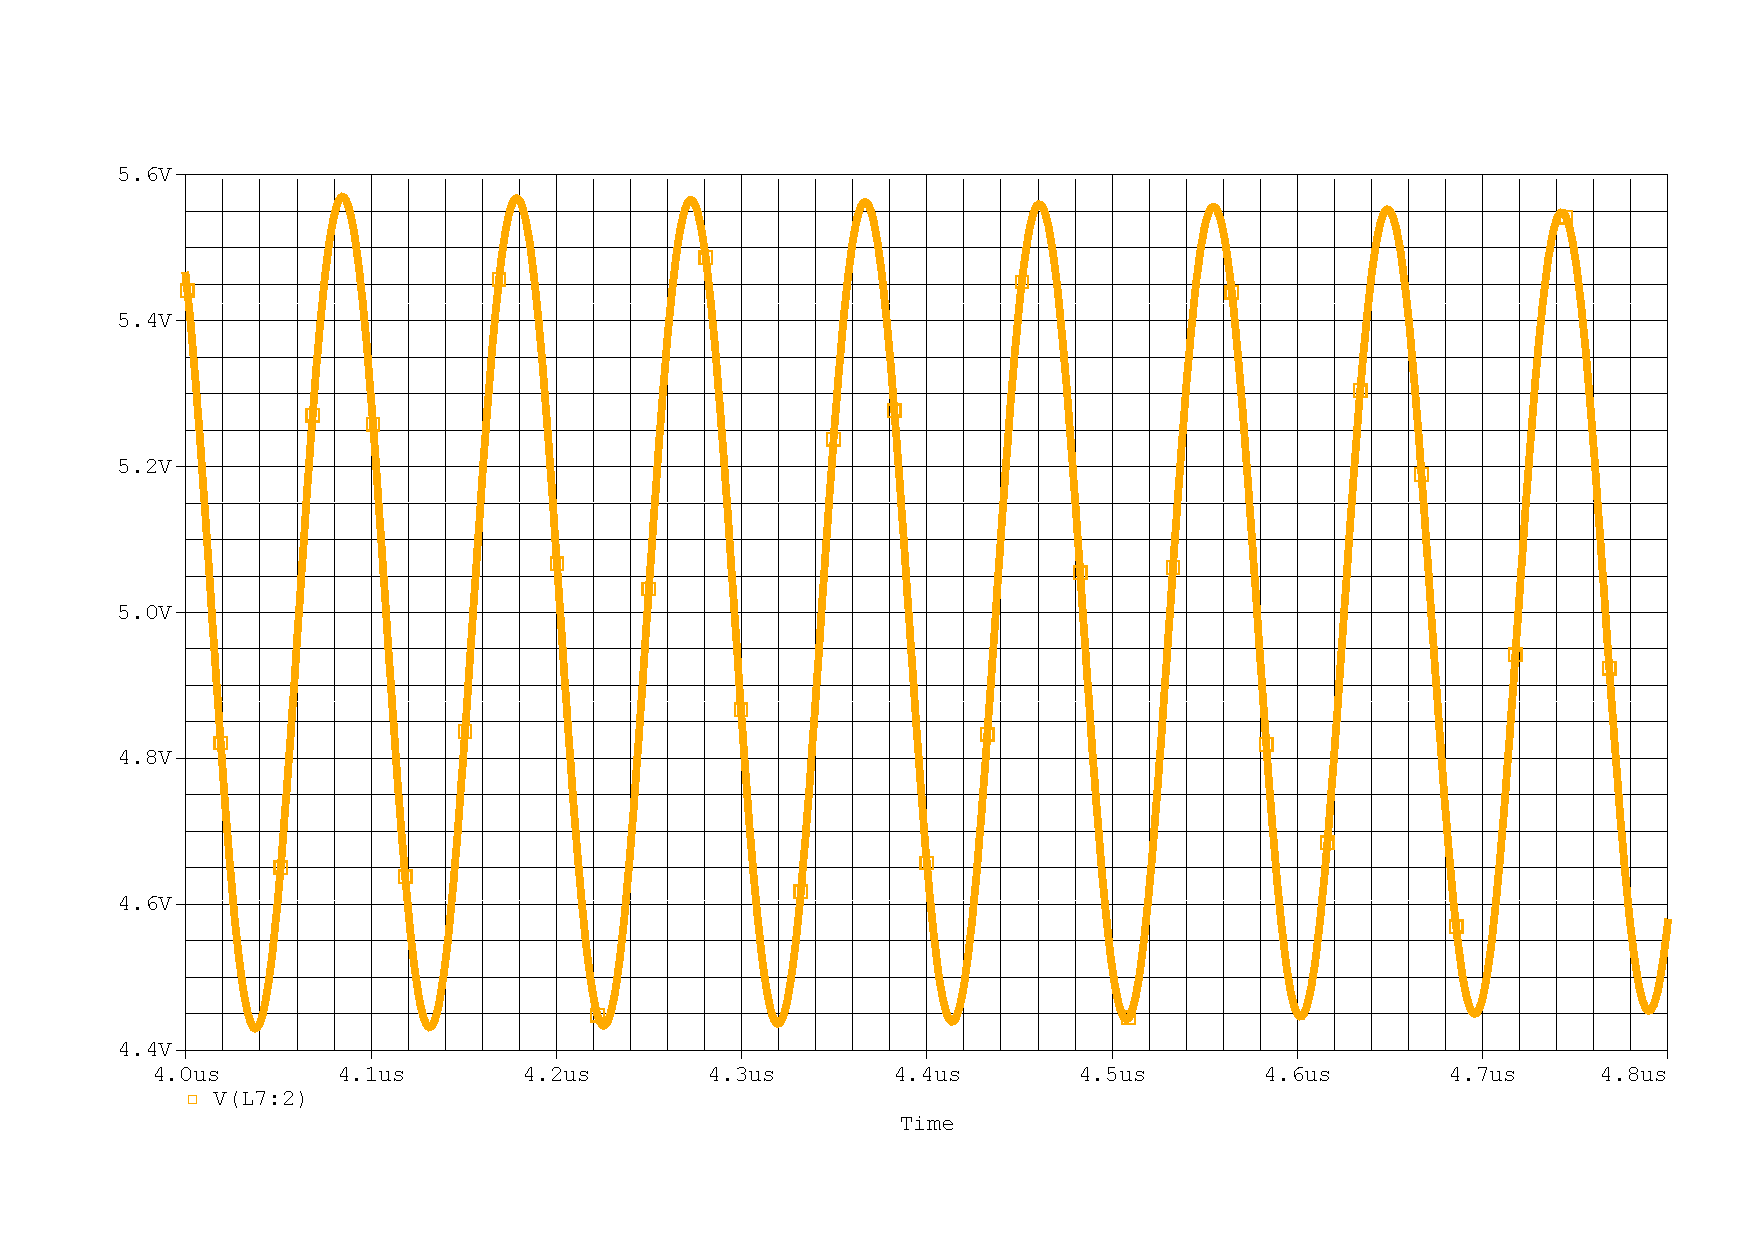
\includegraphics[width=0.42\textwidth]{中放电压波形.pdf}
    }
     \hspace{0.01\linewidth}
      \subfigure[subfigure 1-2][\quad $i_{ipp}=10.95\mathrm{\mu}$A\quad  $i_{opp}=75.616\mathrm{\mu}$A]{
        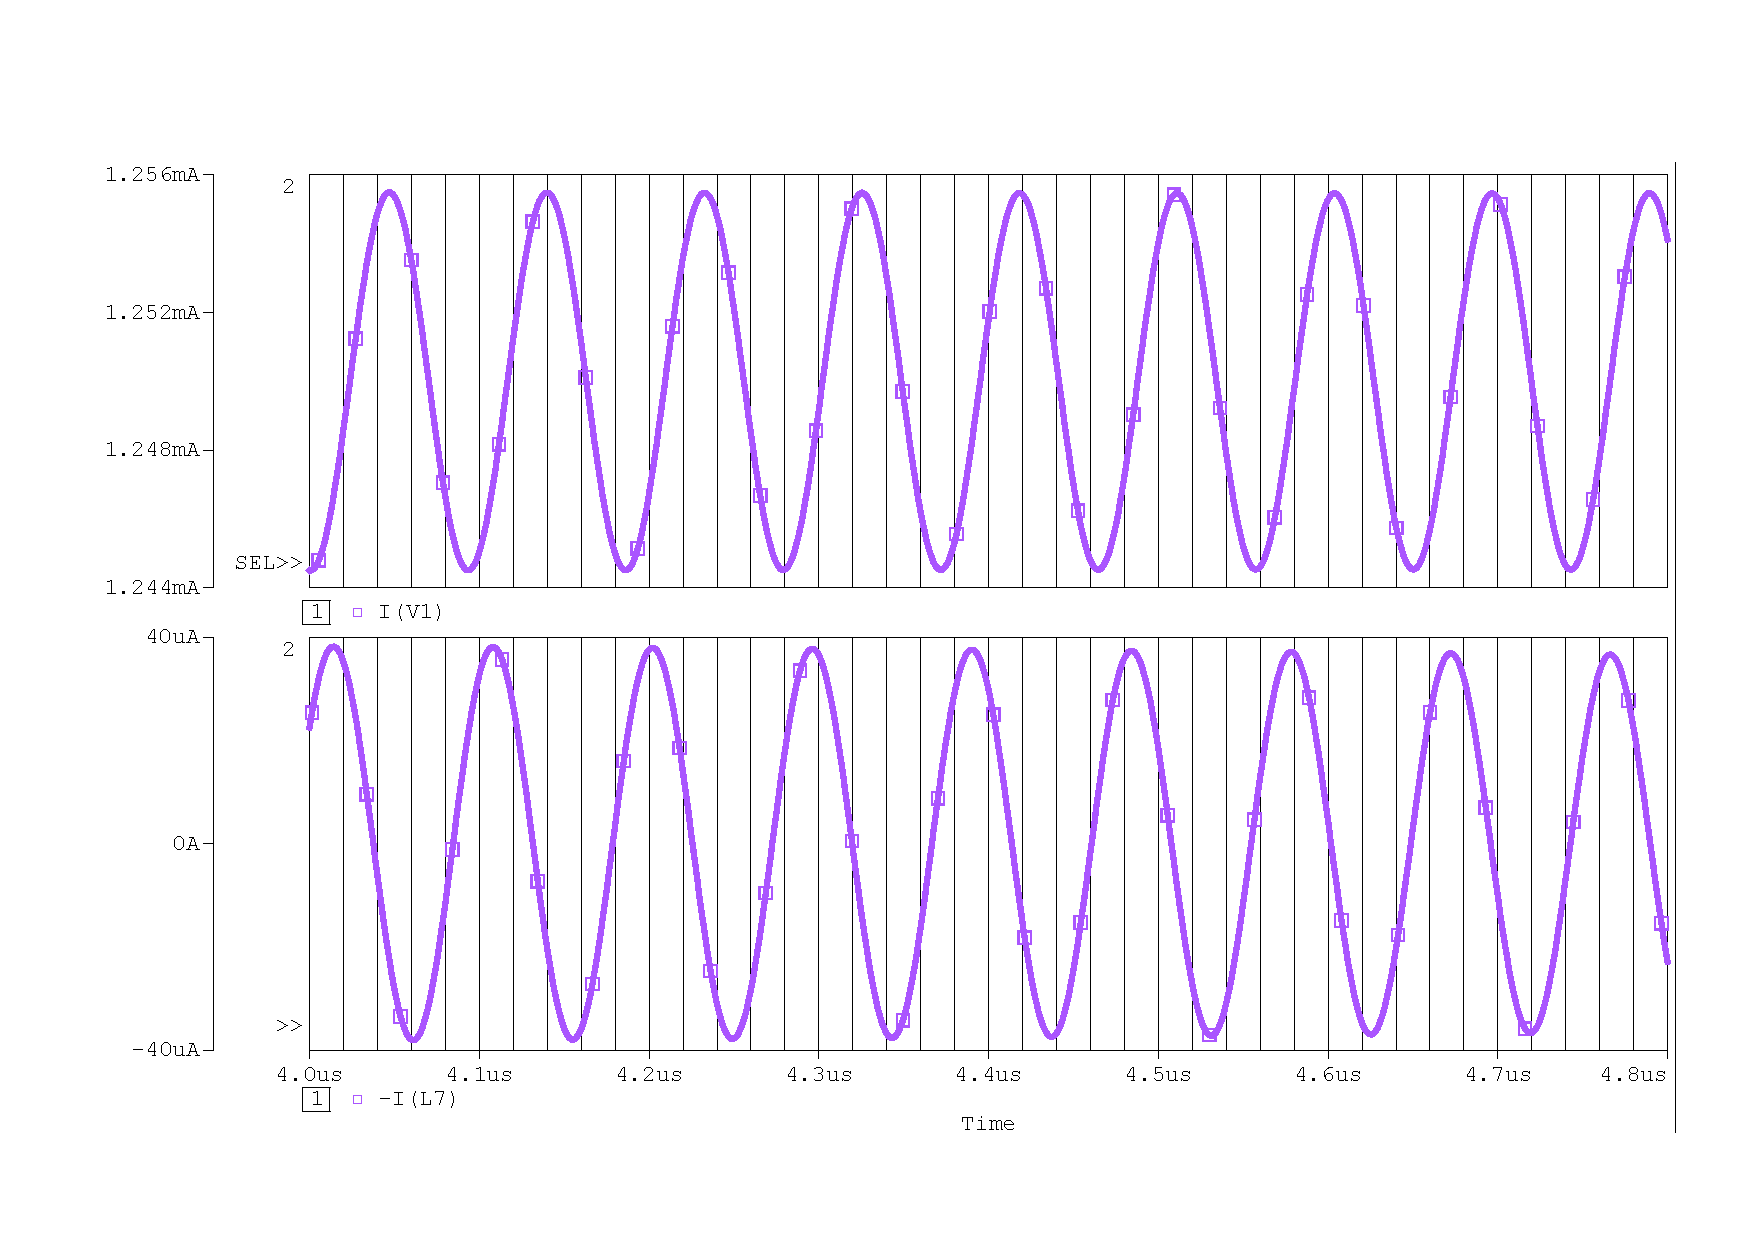
\includegraphics[width=0.42\textwidth]{中放电流波形.pdf}
    }
    \caption{中频放大电路时域仿真}
  \label{中放_wave}
\end{figure}

采用十字光标得到测试电压、电流峰峰值,列表如下:
\begin{table}[H]
    \centering
    \begin{tabular}{ccccc}
    \toprule[1.2pt]
    \midrule
        仿真测量物理量 & 输入电压& 输出电压& 输入电流& 输出电流  \\
        \midrule
        测量值(峰峰值) & 20mV&1.133V&10.96$\mathrm{\mu}$A&75.62$\mathrm{\mu}$A\\
        \bottomrule[1.2pt]
    \end{tabular}
    \caption{中频放大器测量结果}
    \label{中频测量}
\end{table}
从表中看出,中放级对电压的放大效果略高于对电流的放大效果:对电压的放大效果主要通过谐振回路的幅频特性表现,而对电流的放大效果主要由三极管参数决定。

根据表中数据计算中频放大器功率增益,有:
\begin{equation}
    G_p=10\mathrm{lg}(\frac{P_{opp}}{P_{ipp}})=10\mathrm{lg}(\frac{v_{opp}}{v_{ipp}}\cdot\frac{i_{opp}}{i_{ipp}})=10\mathrm{lg}(\frac{1.133}{20\times 10^{-3}}\times \frac{75.62}{10.96})=25.92\mathrm{dB}
    \label{式27}
\end{equation}

将功率增益结果25.92dB与式\ref{中放增益式子}计算结果相对比,式\ref{中放增益式子}所对应的额定功率增益为45.12dB,两者相差较大,这是由于在第一级双调谐电感耦合回路中,为了避免次级反馈引起的谐振频率改变,将电感值减小从而引发的增益下降,但同时保障了10.7MHz中频处得到最大的输出幅值。%\footnote{在实际应用电路中,除了电感耦合问题,还应当考虑插入损耗(insertion loss)与失配损耗(dismatch loss)对功率增益带来的影响。}

\subsubsection{中放级频域仿真}
采用VAC电压源,对中频放大电路在1MHz至200MHz范围内扫频,得到幅频特性曲线如图\ref{中放幅频}所示:
\begin{figure}[H]
    \centering
    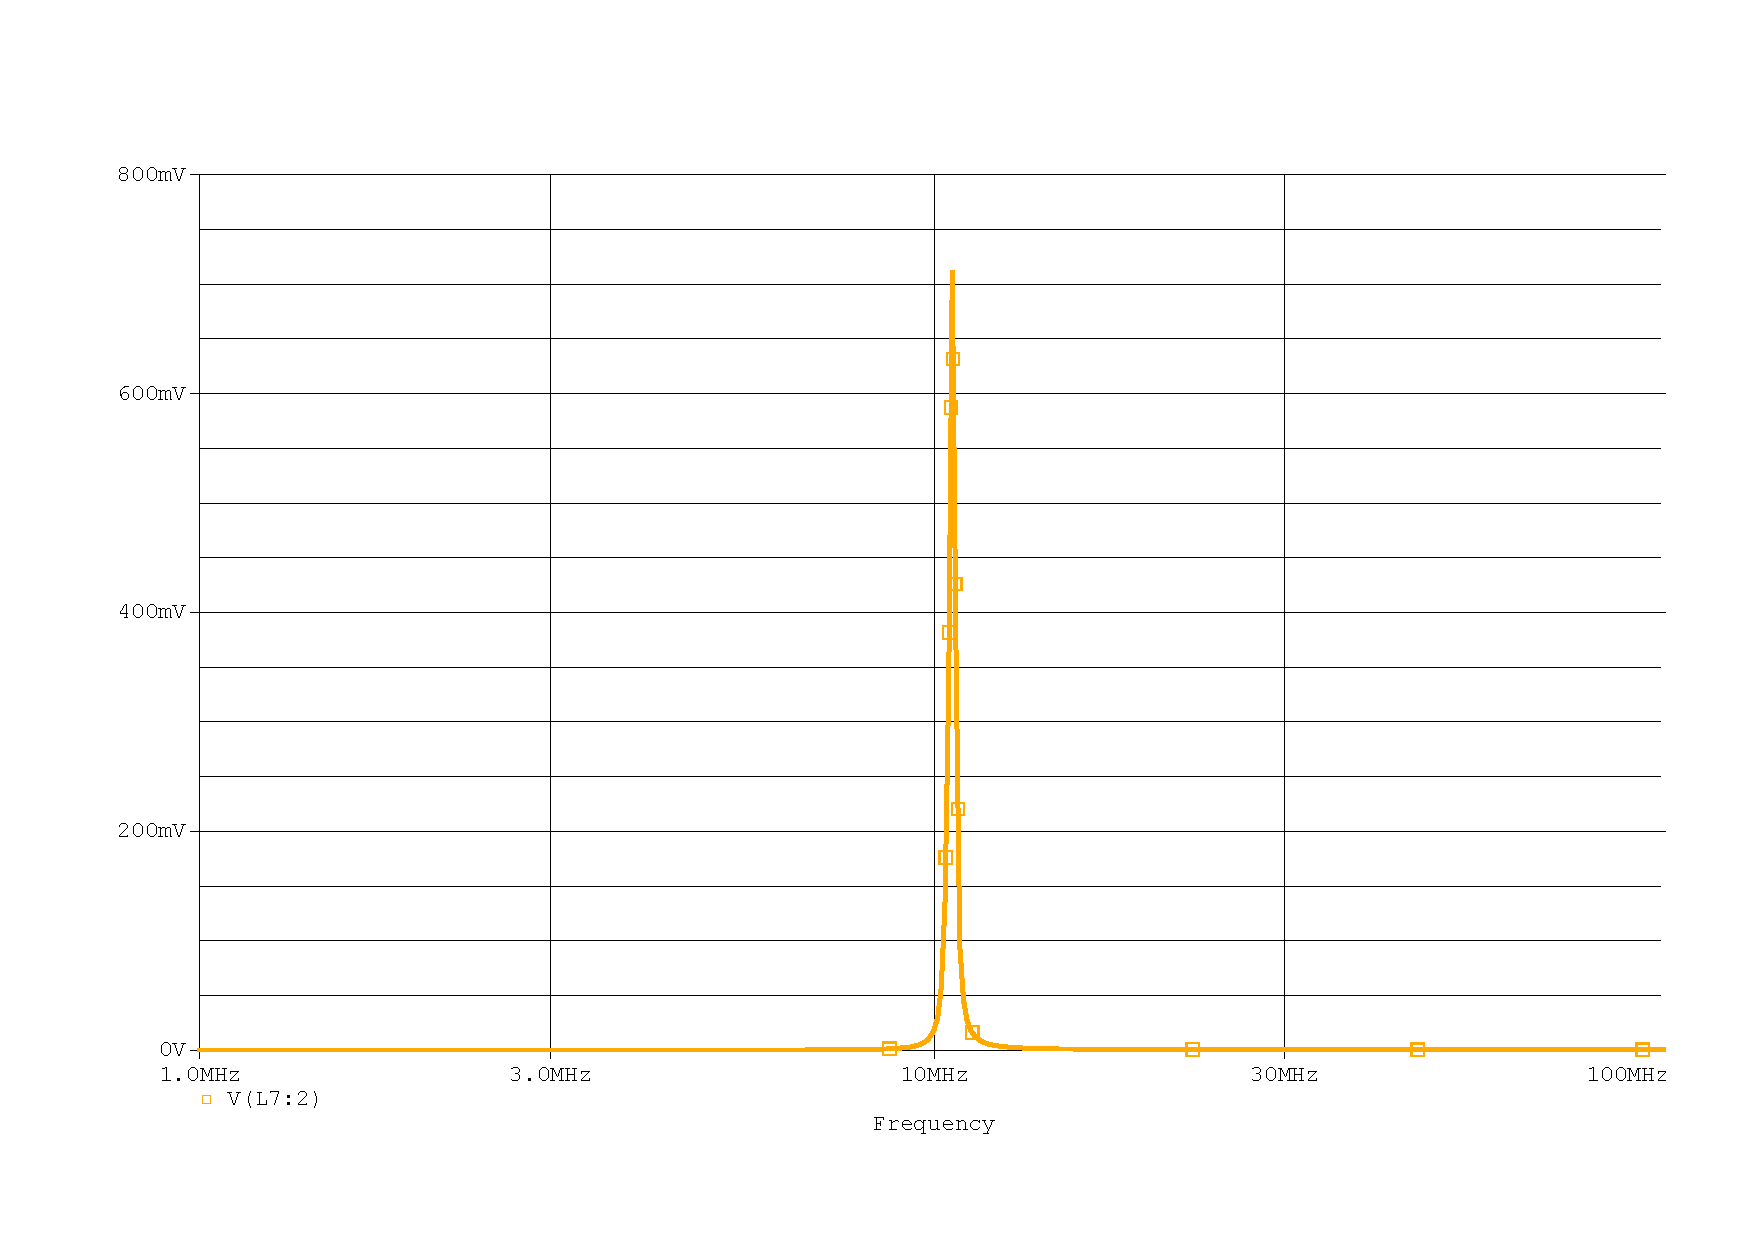
\includegraphics[scale=0.32]{中放仿真频域.pdf}
    \caption{中频放大器幅频特性}
    \label{中放幅频}
\end{figure}
观察到输出端LC回路谐振于中频10.7MHz位置处,测量0.707倍位置处带宽,得到$BW_{mid}=10.67M-10.52M$=150KHz,能够有效地选出最大频偏范围内的频率。




\subsection{解调级仿真}
%test_7.dsn
\textbf{测试频点}:10.7MHz;\textbf{谐振频点}:11.19MHz,10.21MHz

解调级仿真采用时域与频域仿真。时域仿真用以测量解调电路的频-幅变换能力与包络检波效果;频域仿真用以测量解调灵敏度(即鉴频跨导)。

采用两个相同的VSFFM信号源接入解调电路,中间接地,实现上下波形反向叠加。
\begin{figure}[H]
    \centering
    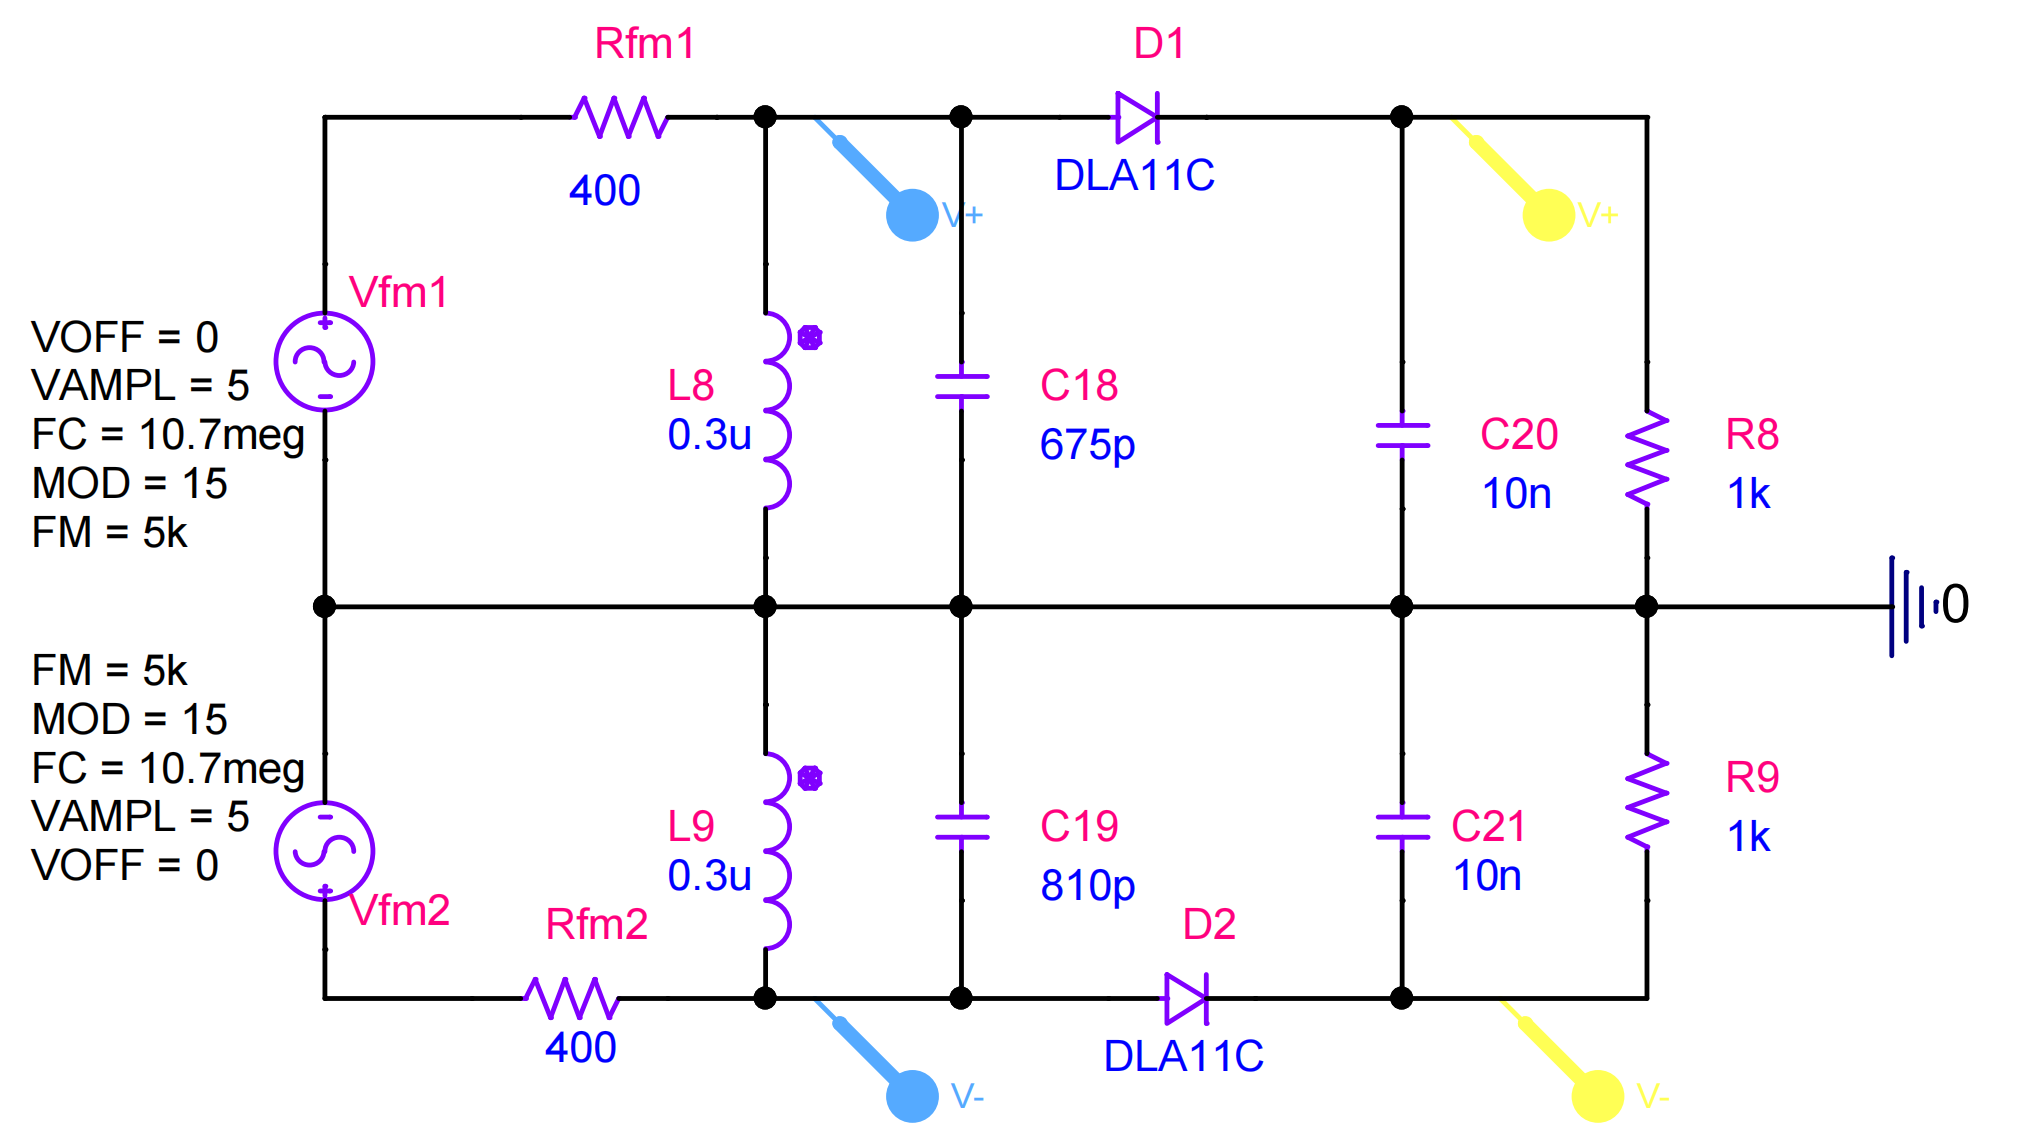
\includegraphics[scale=0.18]{解调仿真电路.png}
    \caption{解调仿真电路}
    \label{解调仿真电路}
\end{figure}


\subsubsection{解调级时域仿真}
如图\ref{解调仿真电路}所示,蓝色表笔指向谐振回路输出端,即频-幅变换输出端电压$v_{FM-AM}$;黄色表笔指向RC回路输出端,即检波输出的调制电压$v_{\Omega}$。

由设计要求,声音带宽为10kHz,即基带信号调制频率中间值F=5kHz
,VSFFM信号源以调制信号中间值输入。为了满足最大频偏要求,根据国家广播FM要求,最大频偏为75kHz,因此设定调制度为15(实际调制度略小于15),包络检波的输出(即黄色波线)应当以调制信号频率的倒数为周期,即$T=\frac{1}{F}=0.2$ms。
\begin{figure}[H]
    \centering
    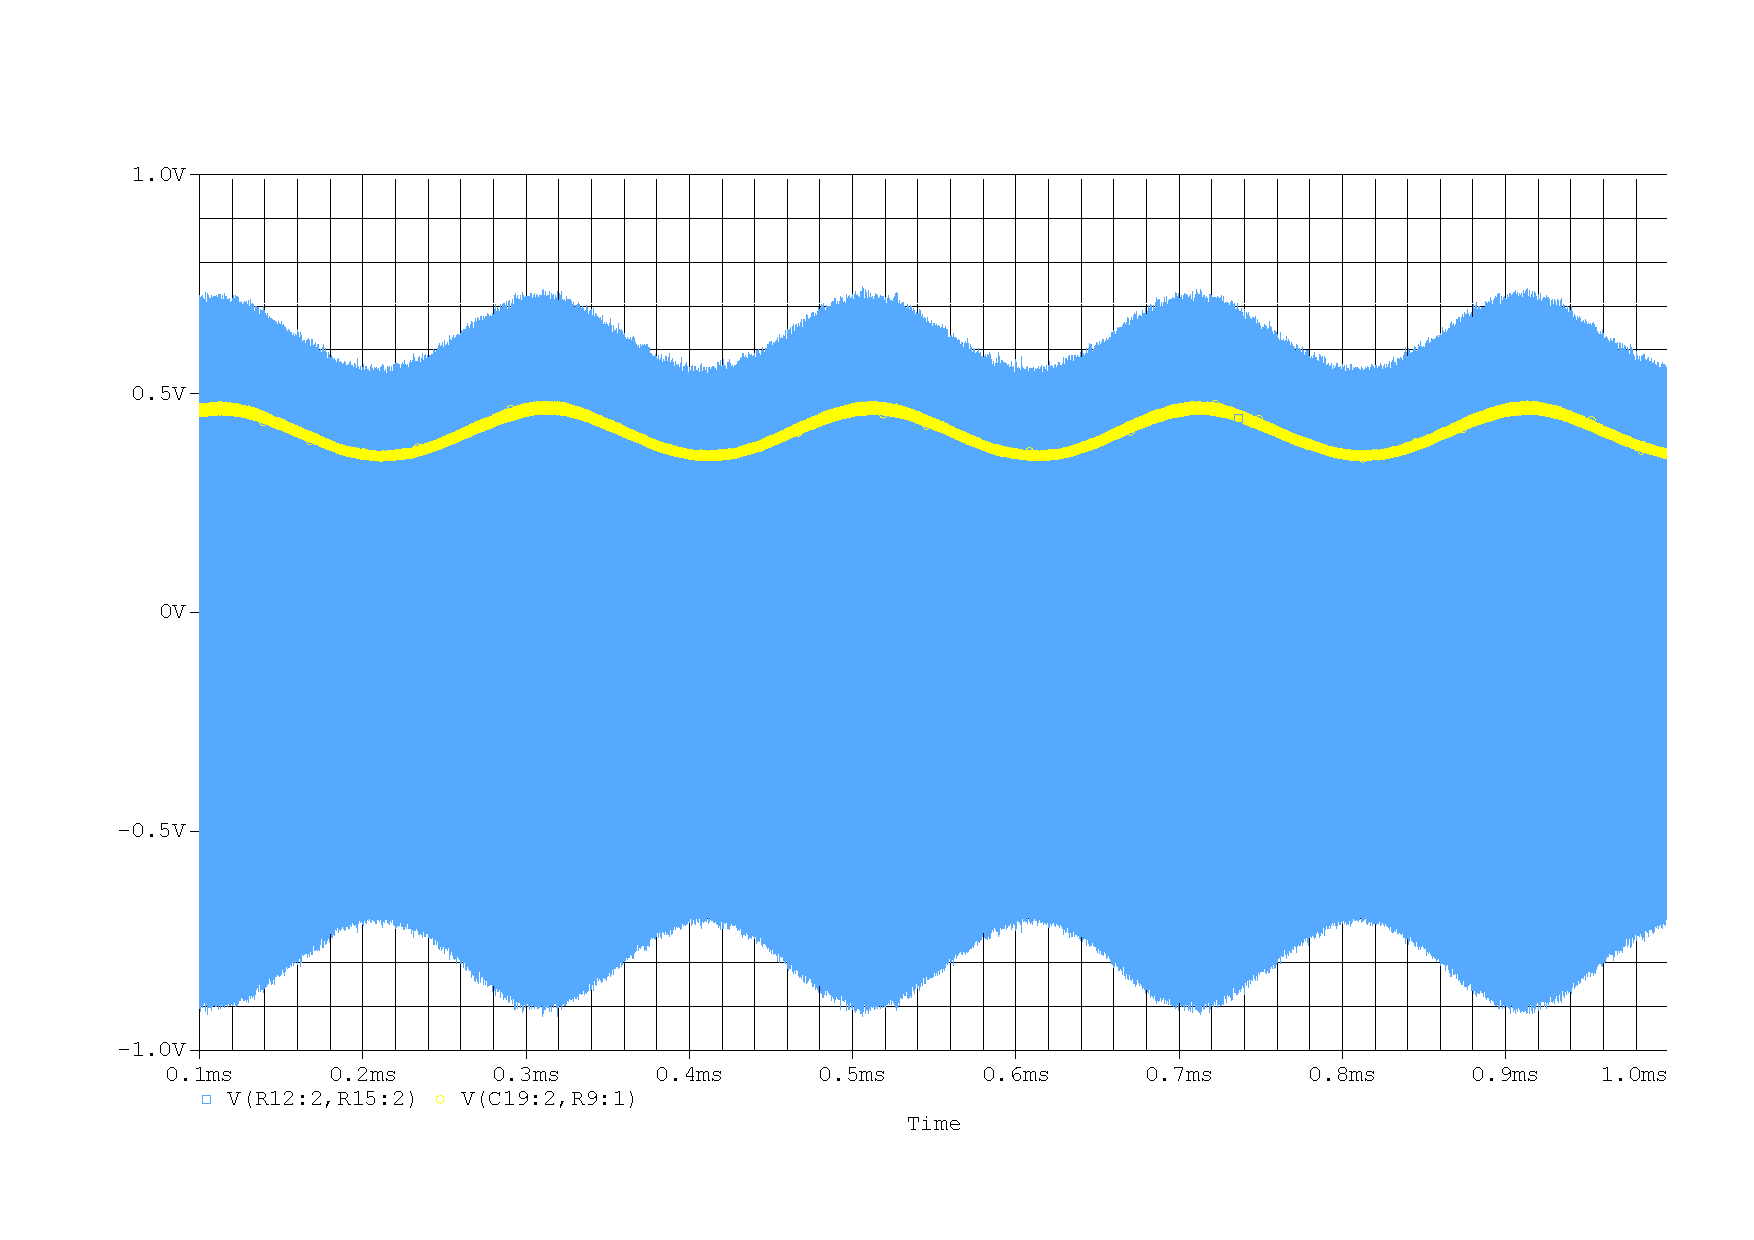
\includegraphics[scale=0.35]{解调时域.pdf}
    \caption{解调时域仿真波形}
    \label{解调时域}
\end{figure}
仿真从0.1ms至1ms
,观察蓝色波形,从输入的调频波已转化为调幅波,幅度每0.2ms作一次周期变化,与假设的调制信号周期一致,表明频-幅转换成功;观察黄色波形,黄色波形滤除了蓝色波形中的载波频率分量,以0.2ms为周期输出正弦波形,表明检波成功,未产生惰性失真与底部切割失真等情形。
\subsubsection{解调级频域仿真}
%%%%%频域S曲线需要Web模拟
将电压源换为VAC,分别用红色表笔及蓝色表笔测量两个LC回路的幅频曲线,如下所示:
\begin{figure}[H]
    \centering
    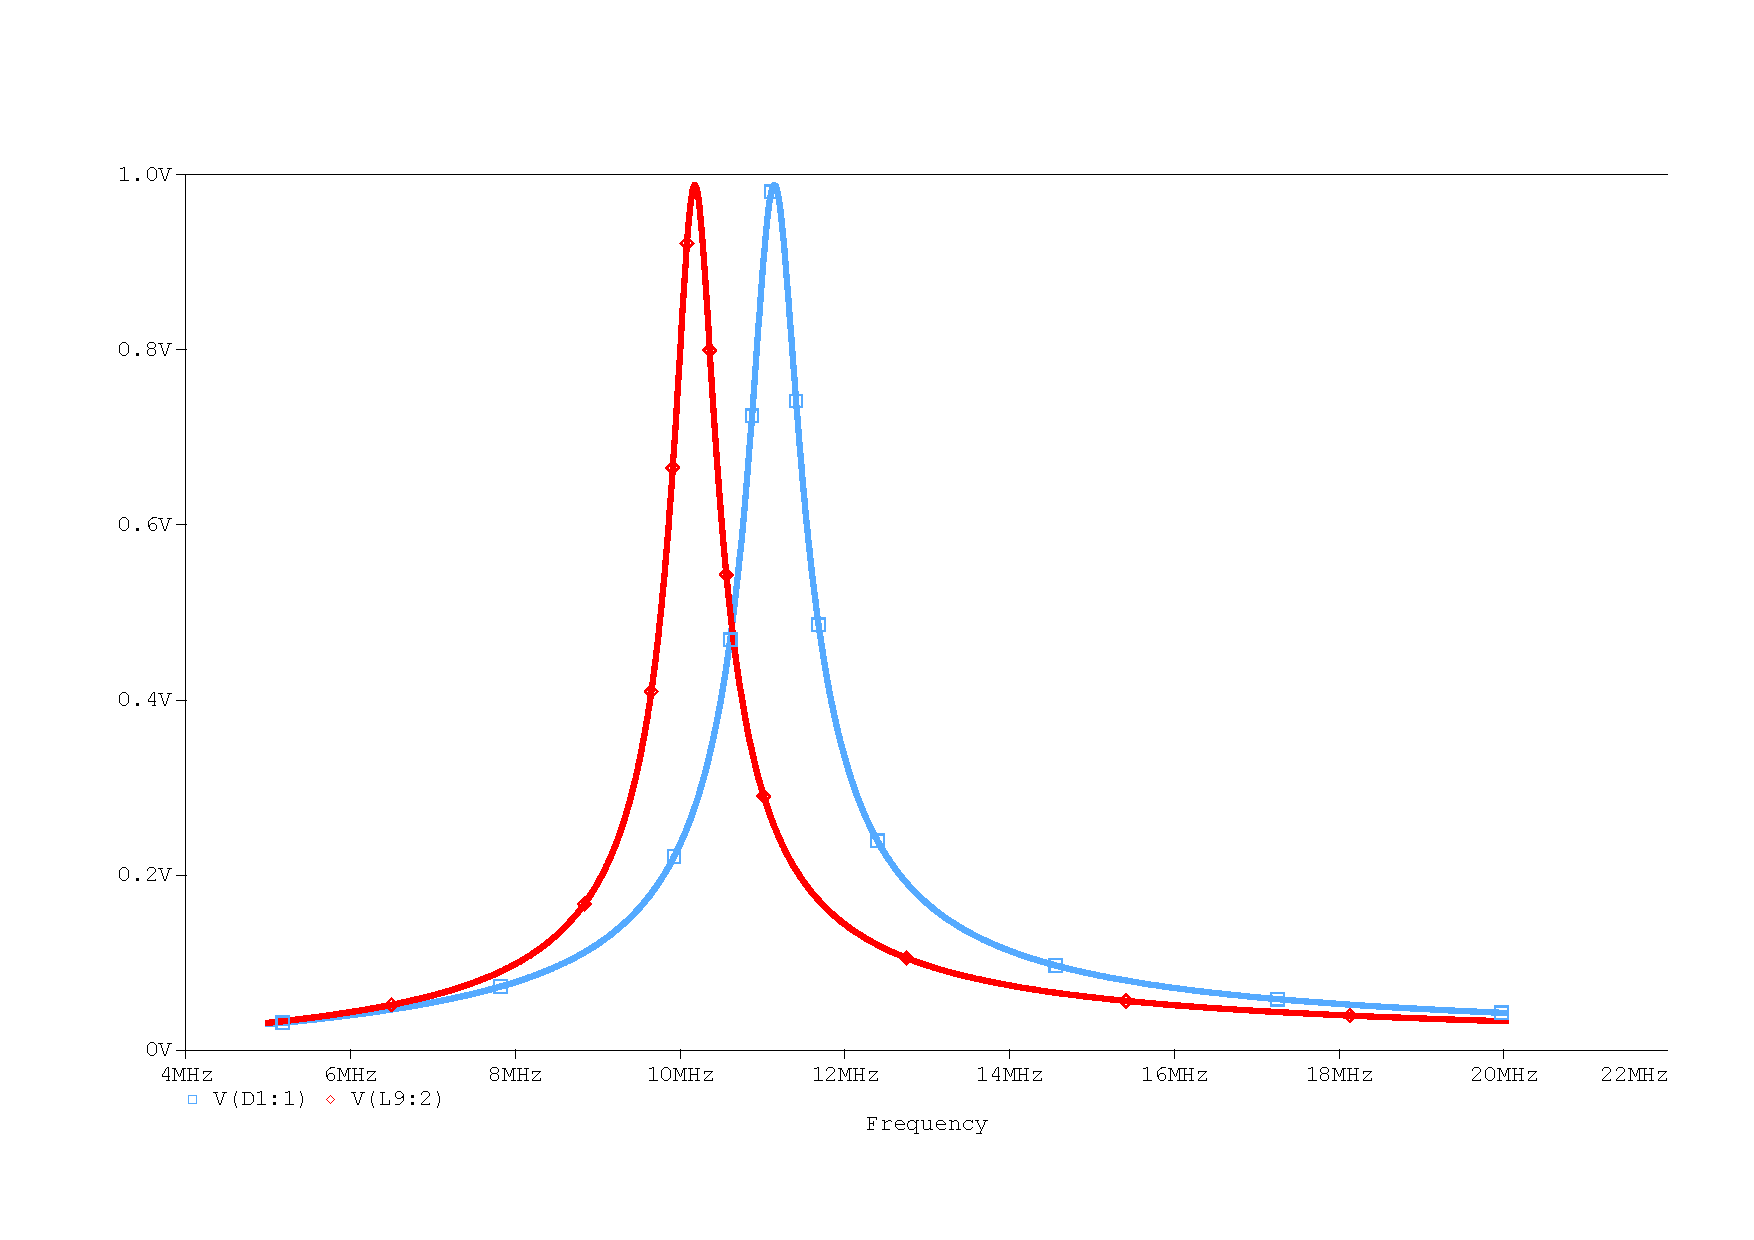
\includegraphics[scale=0.32]{解调频域仿真.pdf}
    \caption{解调电路频域仿真}
    \label{解调频域}
\end{figure}

利用描点软件\footnote{Pspice OrCAD无法直接显示幅频曲线的合成结果,采用Origin对时域扫描点坐标进行描点合成。},合成两个幅频特性曲线,如下所示:
\begin{figure}[H]
    \centering
    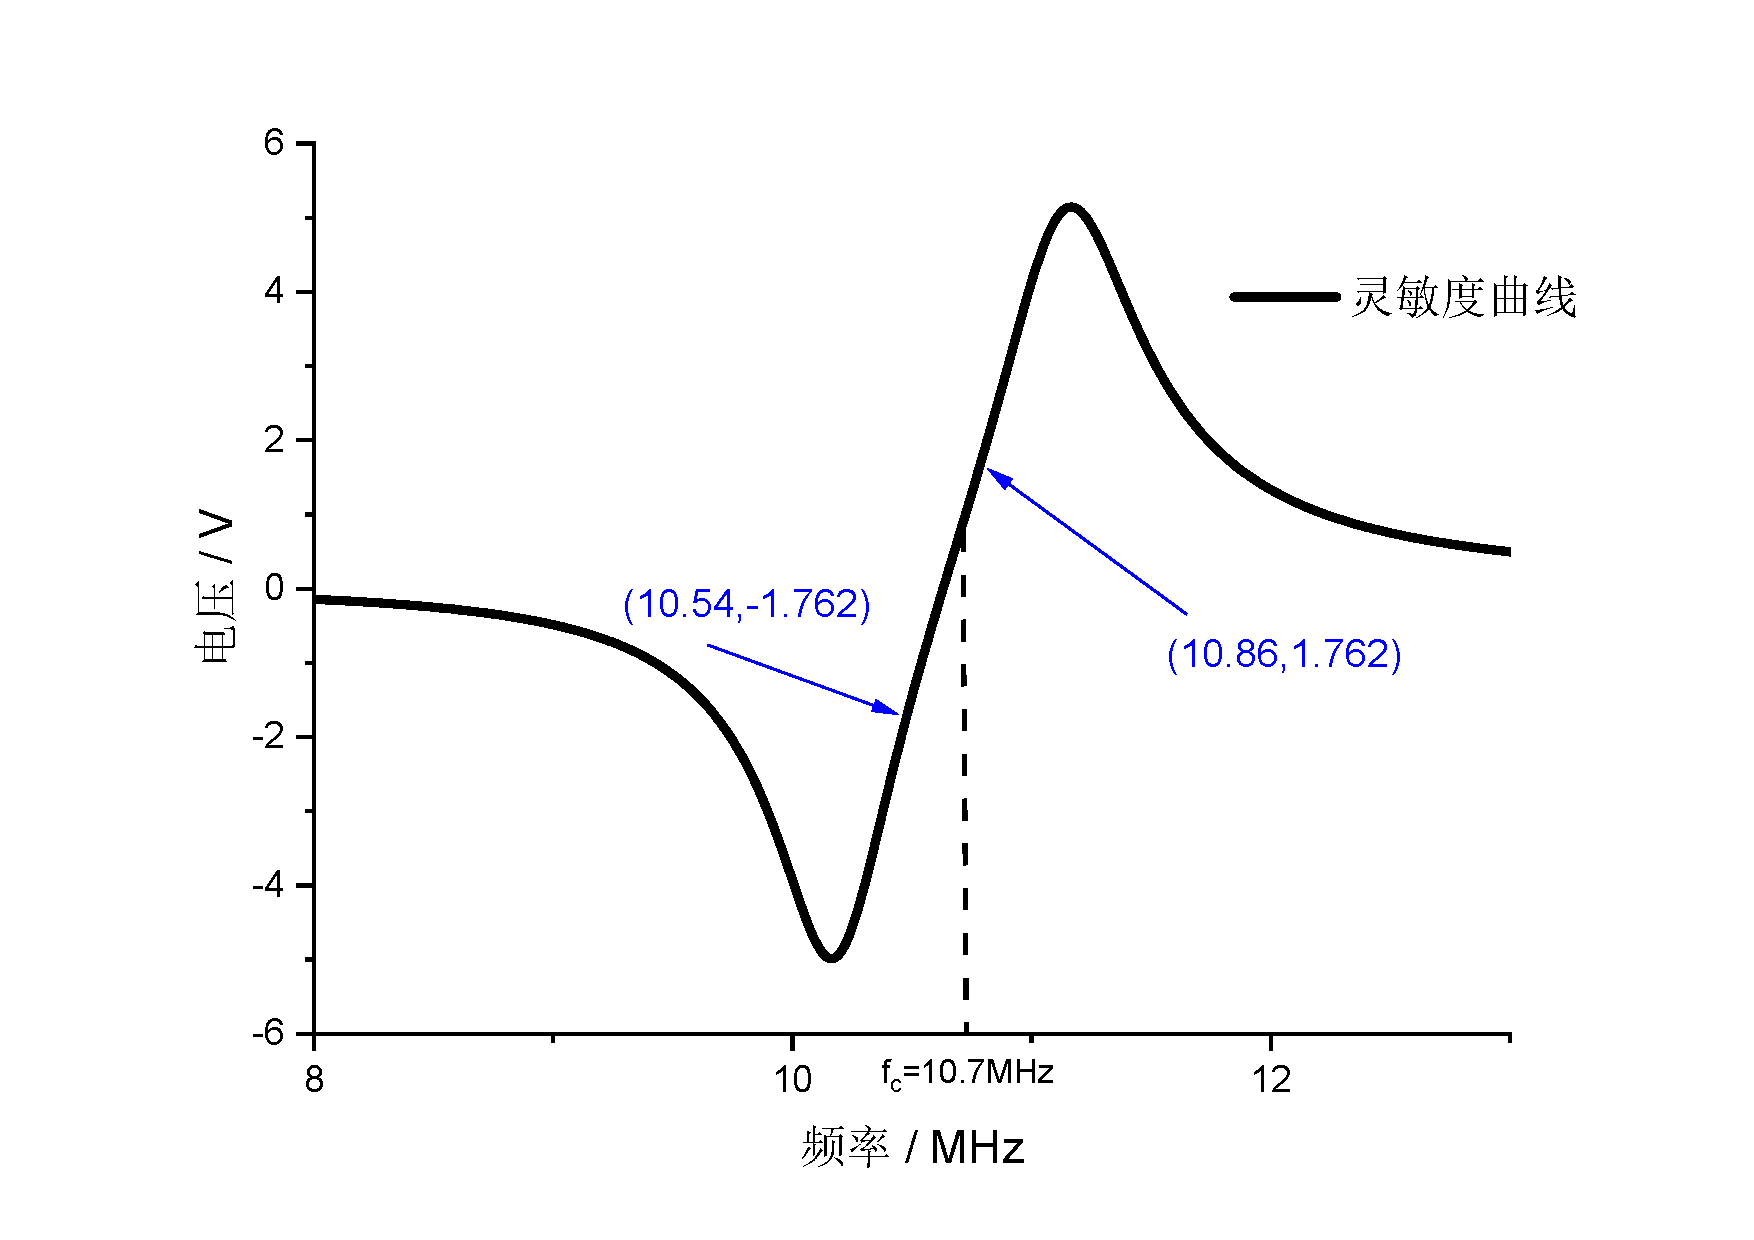
\includegraphics[scale=0.36]{灵敏度曲线.pdf}
    \caption{灵敏度曲线}
    \label{灵敏度曲线}
\end{figure}
由式\ref{FM带宽},找出载波10.7MHz左右两侧频率最大偏离点(以$BW_{FM}=160-170$KHz计),对应图中蓝色箭头所指位置。在包含频偏及基带频率的频率范围内可求得鉴频跨导如下:
\begin{equation}
    g_d=\frac{\Delta v_o}{\Delta f}=\frac{1.762-(-1.762)}{(10.86-10.54)\times 10^{6}}\approx 11.0125\mathrm{\mu}V
    \label{式28}
\end{equation}
从而灵敏度为11.0125$\mathrm{\mu}$V,满足灵敏度不低于10$\mathrm{\mu}$V的设计要求\footnote{仿真过程中,发现选取更接近中频的回路谐振频点可以得到更大的灵敏度,但这建立在线性程度被破坏的基础上。}。

由此可知,灵敏度不仅对LC回路带宽的设计有要求,也需要中放级有足够的增益;另一方面,为了确保幅频特性的中间部分有足够的线性度,不能选取足够接近的失谐频点。

\subsection{低放级仿真}
%%difang.dsn page2
低放级仿真包含时域及频域仿真:时域仿真用以测试电压、电流的幅度,以确定低放级功率;频域仿真用以测试其带宽,以确保声音频率均能通过。
\subsubsection{低放级时域仿真}
 \textbf{测试频点}:5kHz
 
 由设计要求,声音带宽为10kHz,假定声音频率在0-10kHz之间平均分布,以平均值5kHz作为低放级测试频率。

仿真电路如下所示:
\begin{figure}[H]
    \centering
    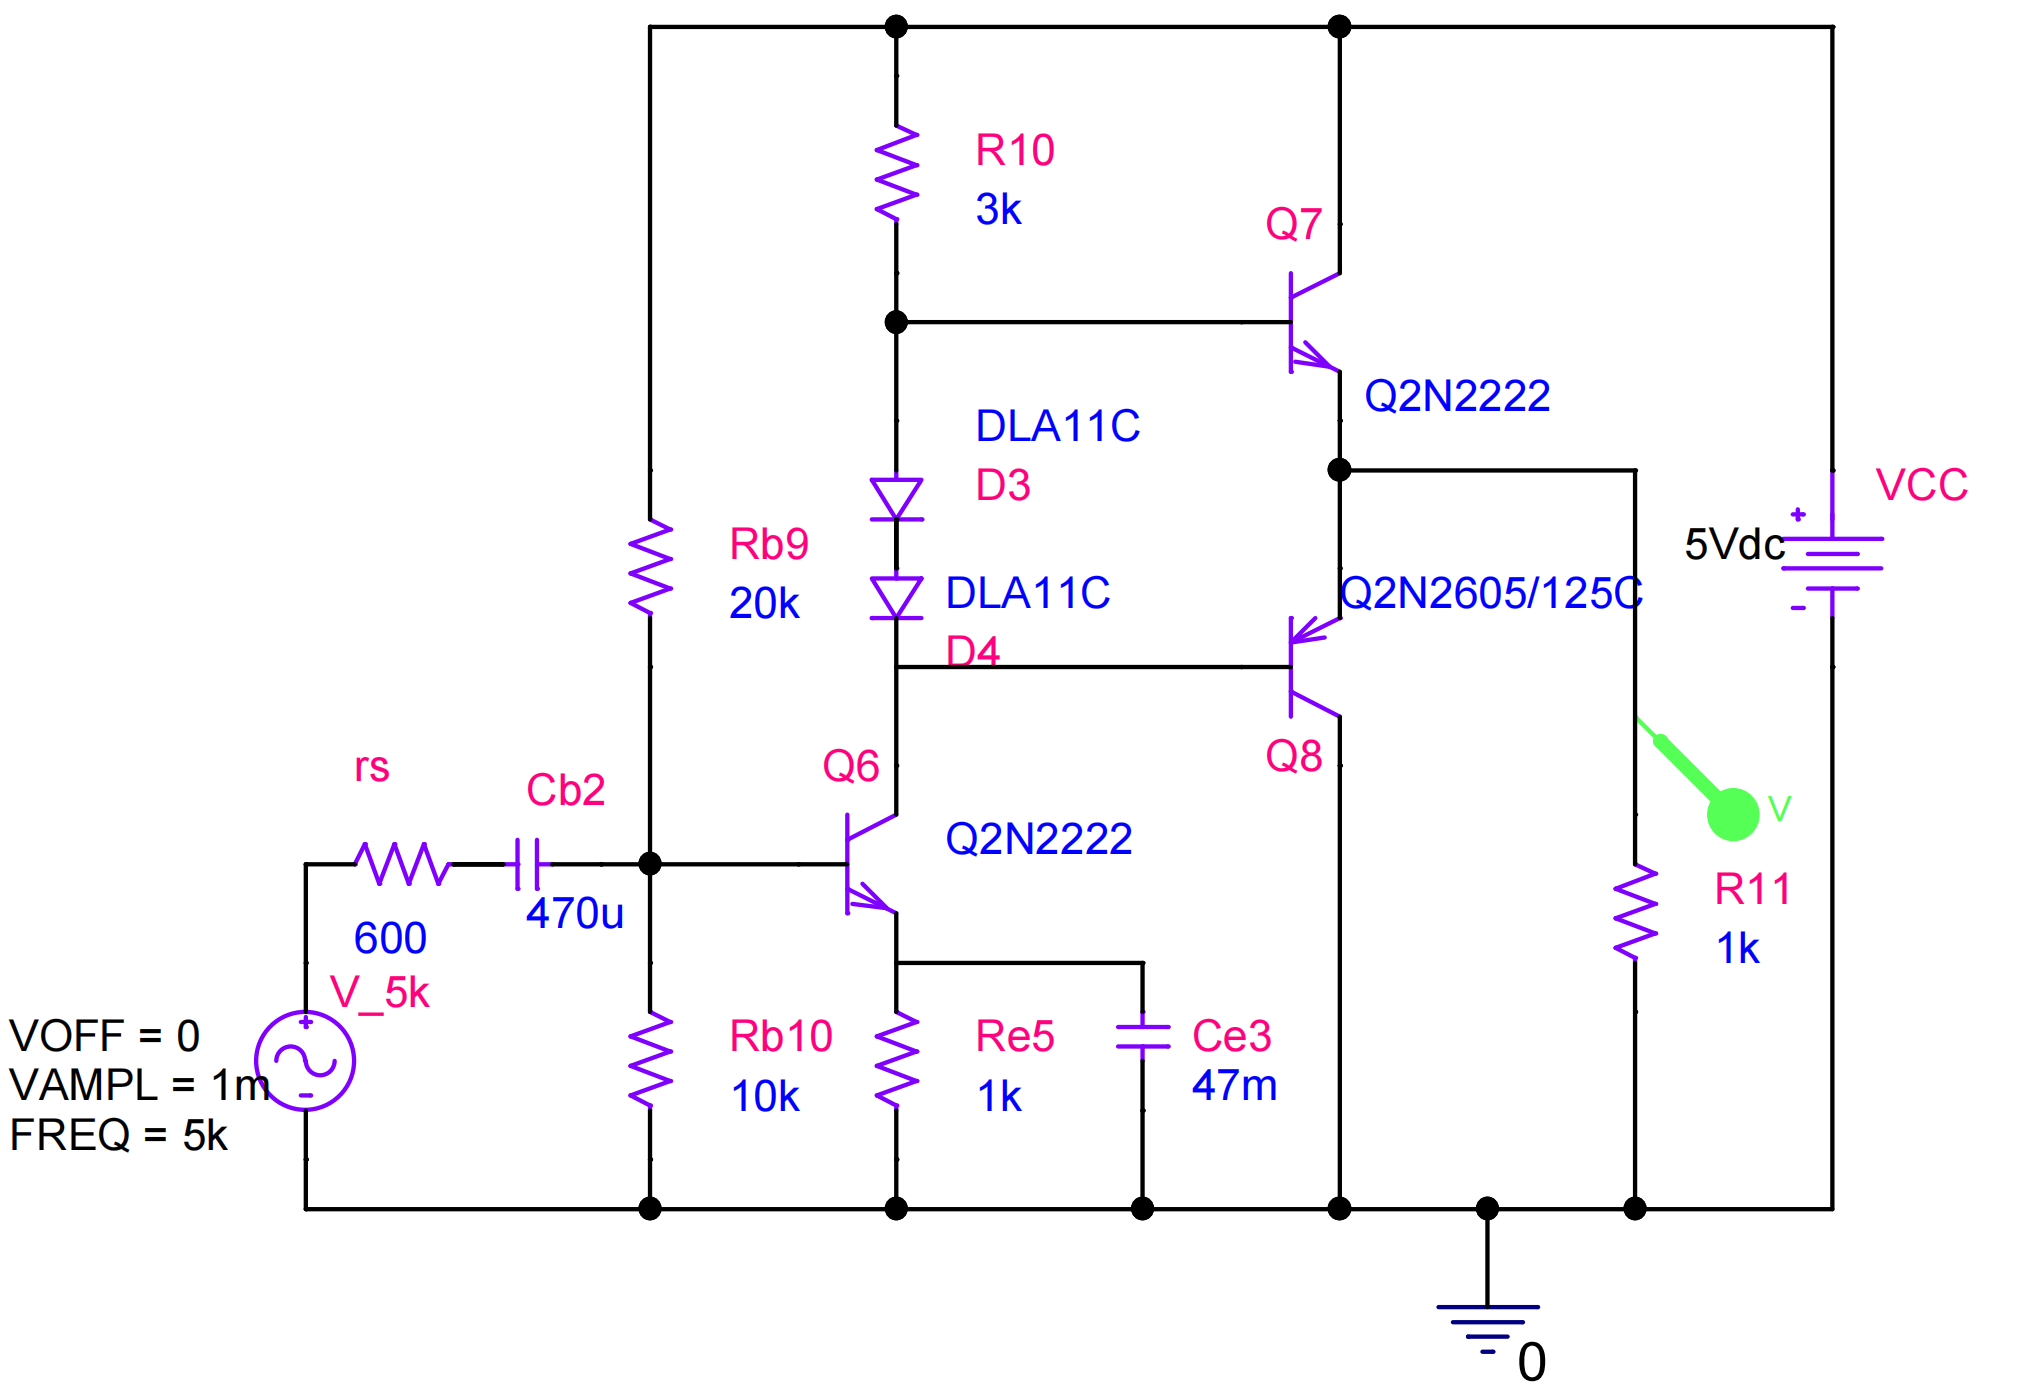
\includegraphics[scale=0.16]{低放仿真.png}
    \caption{低放级仿真电路}
    \label{低放仿真电路}
\end{figure}
如图\ref{低放仿真电路}所示,绿色表笔指向互补电路输出端。按甲乙类功放原理,第一级前置放大输出电压$v_{o1}$近似等于$v_{o2}$,因此仅需测量后级。

将输入端以振动在5kHz频点的电压源接入,电压幅值为1mV。分别测量输出电压(绿表笔)与输出电流(橙表笔),波形如下所示:
\begin{figure}[H]
    \centering
    \subfigure[subfigure 1-1][${v_{o}}_{pp}$=167mV]{
        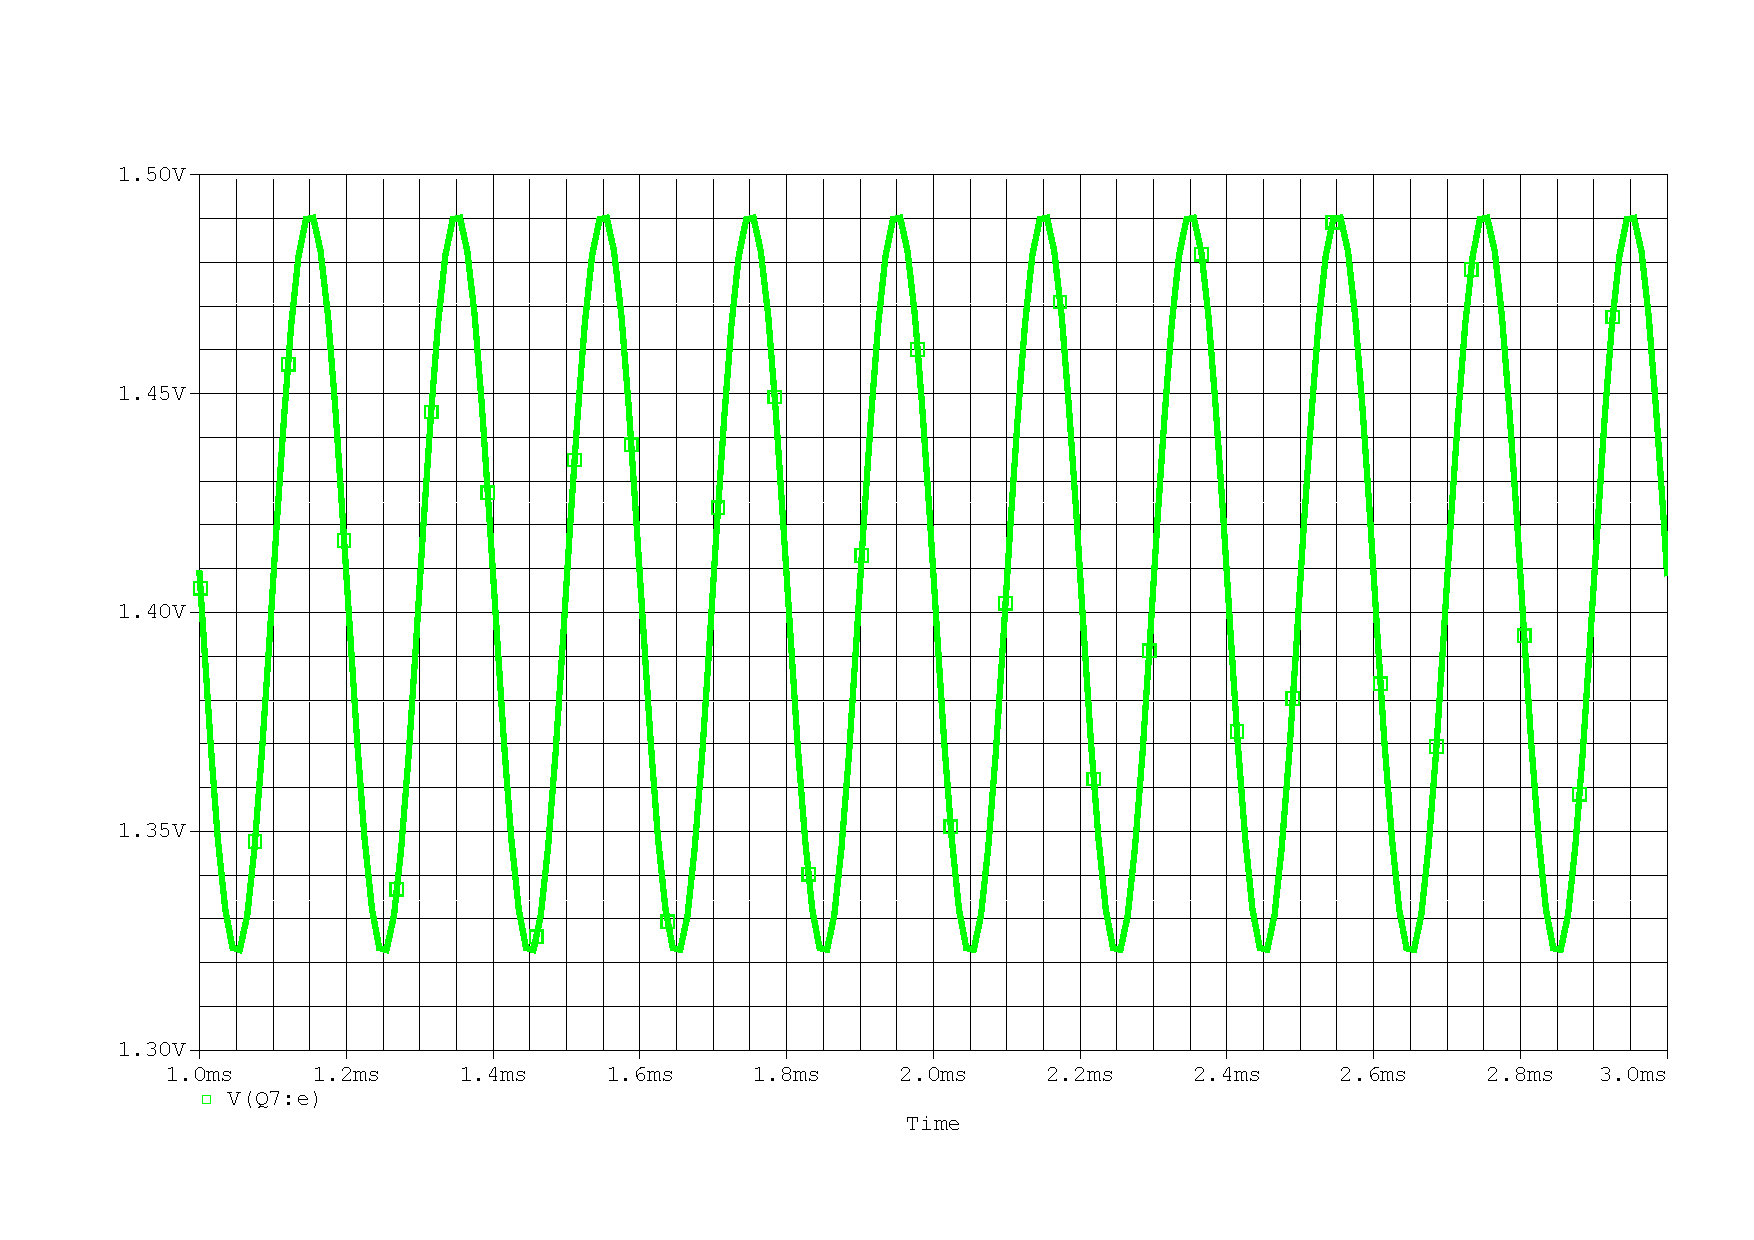
\includegraphics[width=0.42\textwidth]{低放仿真电压.pdf}
    }
     \hspace{0.01\linewidth}
      \subfigure[subfigure 1-2][\quad $i_{ipp}=0.615\mathrm{\mu}$A  \quad     $i_{opp}=167.10\mathrm{\mu}$A]{
        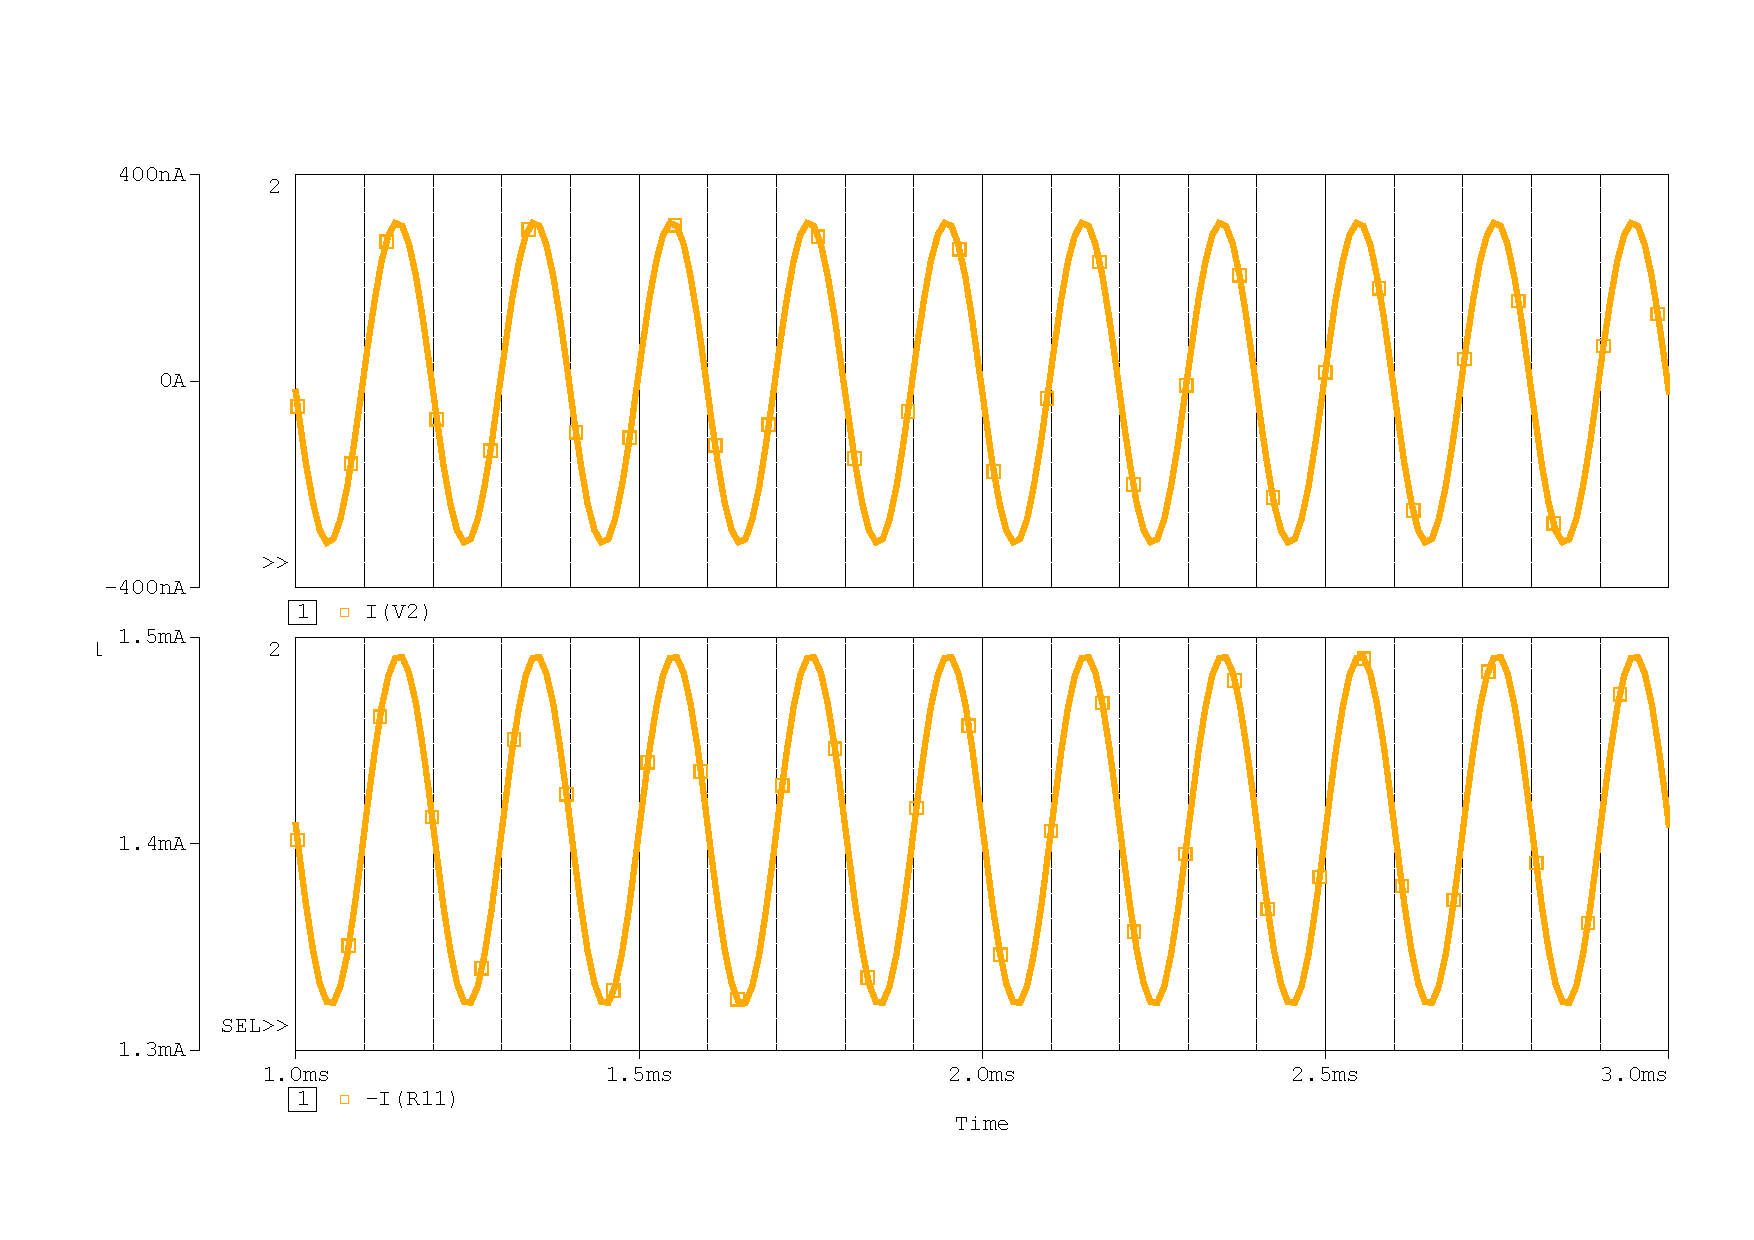
\includegraphics[width=0.42\textwidth]{低放仿真电流.pdf}
    }
    \caption{低频放大电路时域仿真}
  \label{低放时域}
\end{figure}


左上子图中测量得到负载端输出电压$v_{opp}=167$mV,右上子图中测量得到负载端输出电流$i_{opp}=167.10\mu$A,其对应的功率增益
\begin{equation}
    G_{p}(\mathrm{dB})=10\mathrm{lg}(\frac{v_{opp}}{v_{ipp}}\cdot \frac{i_{opp}}{i_{ipp}})=10\mathrm{lg}(\frac{167}{2}\times\frac{167.10}{0.615})\approx43.6\mathrm{dB}
    \label{式29}
\end{equation}

\subsubsection{低放级频域仿真}
将仿真电压源换为VAC(单位幅值1V),在0Hz至10kHz范围内扫频测量电压输出幅度,如图\ref{低放扫频}所示:
\begin{figure}[H]
    \centering
    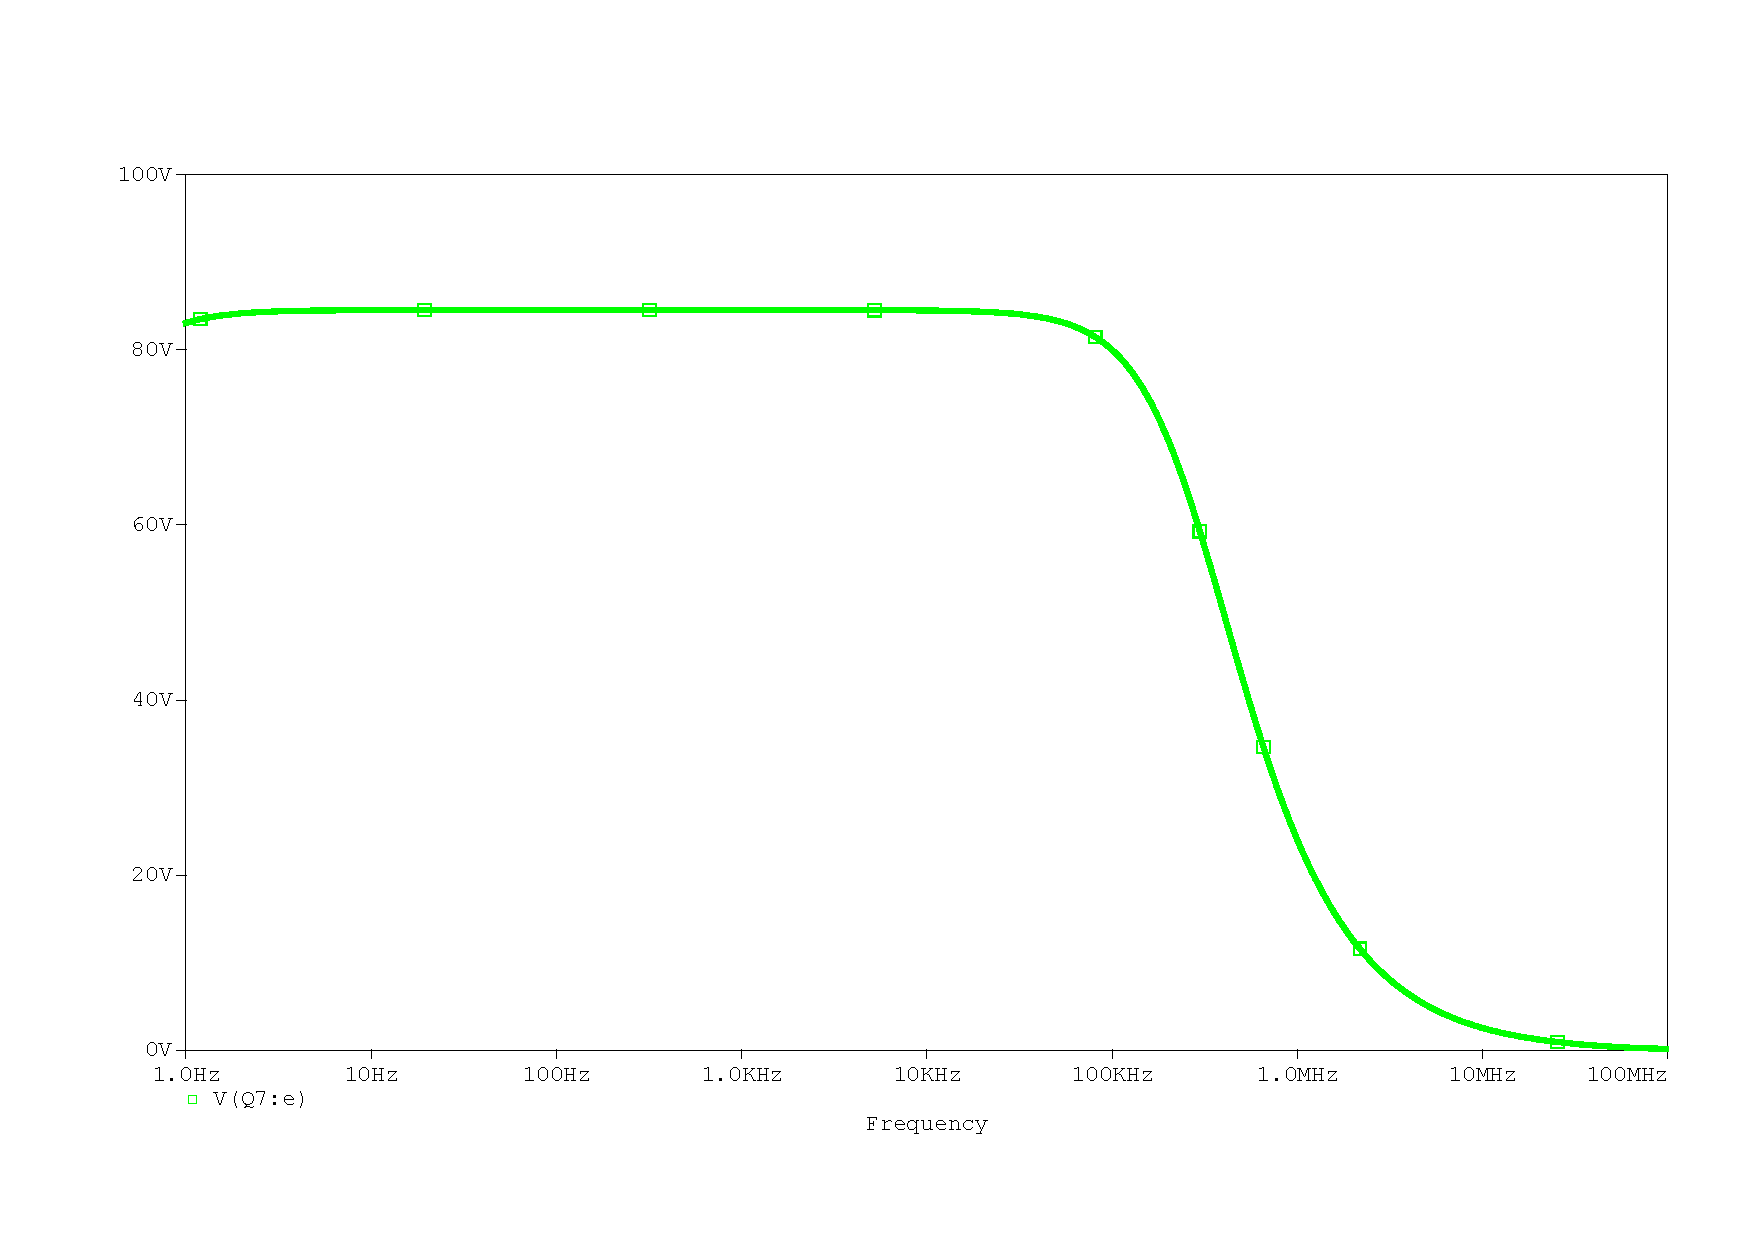
\includegraphics[scale=0.3]{低放频域仿真.pdf}
    \caption{低放级频域仿真}
    \label{低放扫频}
\end{figure}

观察波形,较大的旁路电容保证了下截止频率尽可能地小,使通频带宽度大大增加,在0Hz至10kHz的声音频率范围内都能有效地对信号进行放大。

\subsection{整机仿真}
将收音机各部分仿真板块按图\ref{横板总电路}连接,天线端用仿真信号源VSFFM接入,各板块之间利用变压器耦合以实现阻抗匹配,对整机接收效果进行测试,仿真图如图\ref{整机仿真}所示\footnote{电感$L_7$为电感$L_8,L_9$的前级,出于版面考虑,将解调与低放电路画在下方。}:
\begin{figure}[H]
    \centering
    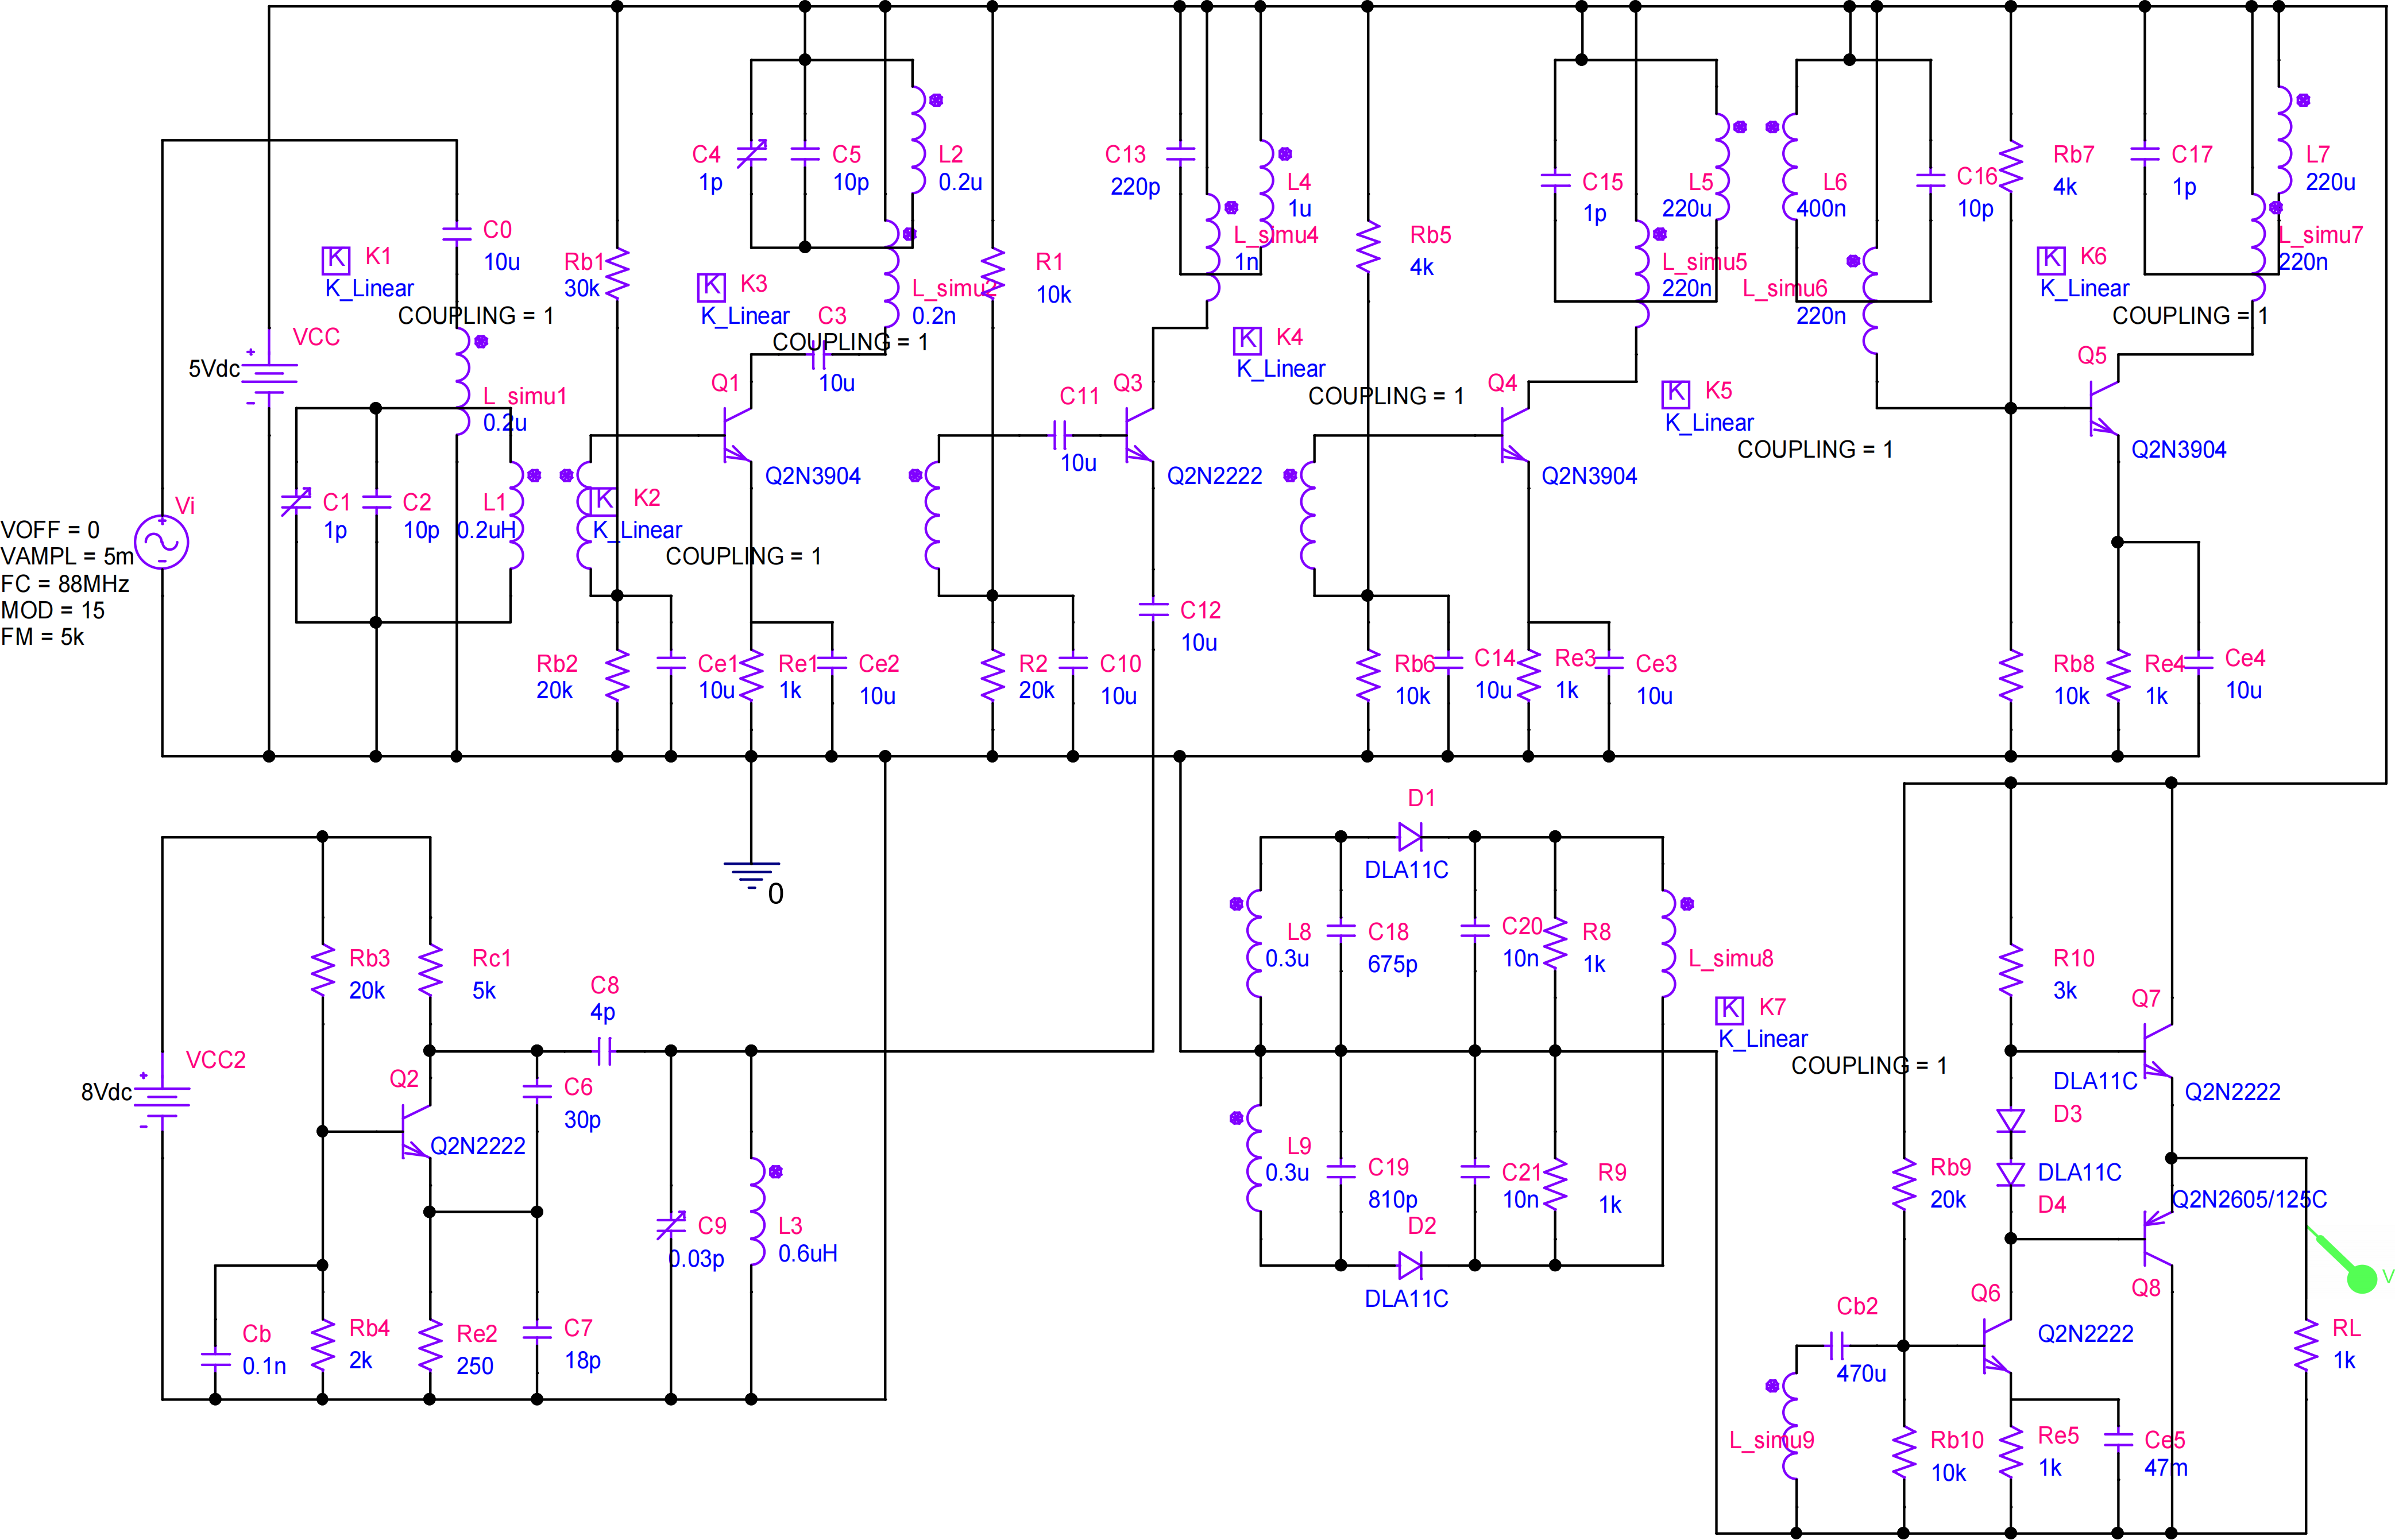
\includegraphics[scale=0.11]{整机仿真.png}
    \caption{整机仿真电路}
    \label{整机仿真}
\end{figure}

为了测试FM收音机设计电路对工作频率之内及工作频率之外的信号的输出效果,分别用如下四组输入频率参数测试整机电路:
\begin{table}[H]
    \centering
    \begin{tabular}{p{5cm}rr}
    \toprule[1.2pt]
    \midrule
    测试频率组组号 & 天线载波频率$f_C$  &   音频信号频率$F$  \\
         \midrule
                 组1 & $70\mathrm{MHz}$   &  5kHz \\
         组2 &   $90\mathrm{MHz}$   &  5kHz \\
         组3 &   $110\mathrm{MHz}$   & 8kHz  \\
         组4&   $130\mathrm{MHz}$   &  8kHz \\
         \bottomrule[1.2pt]
    \end{tabular}
    \caption{频率测试组号}
    \label{整机测试}
\end{table}
得到波形如图\ref{整机测试结果}所示:

\begin{figure}[H]
    \centering
    \subfigure[subfigure 1-1][${v_{o}}_{pp}=82\maathrm{\mu}$V]{
        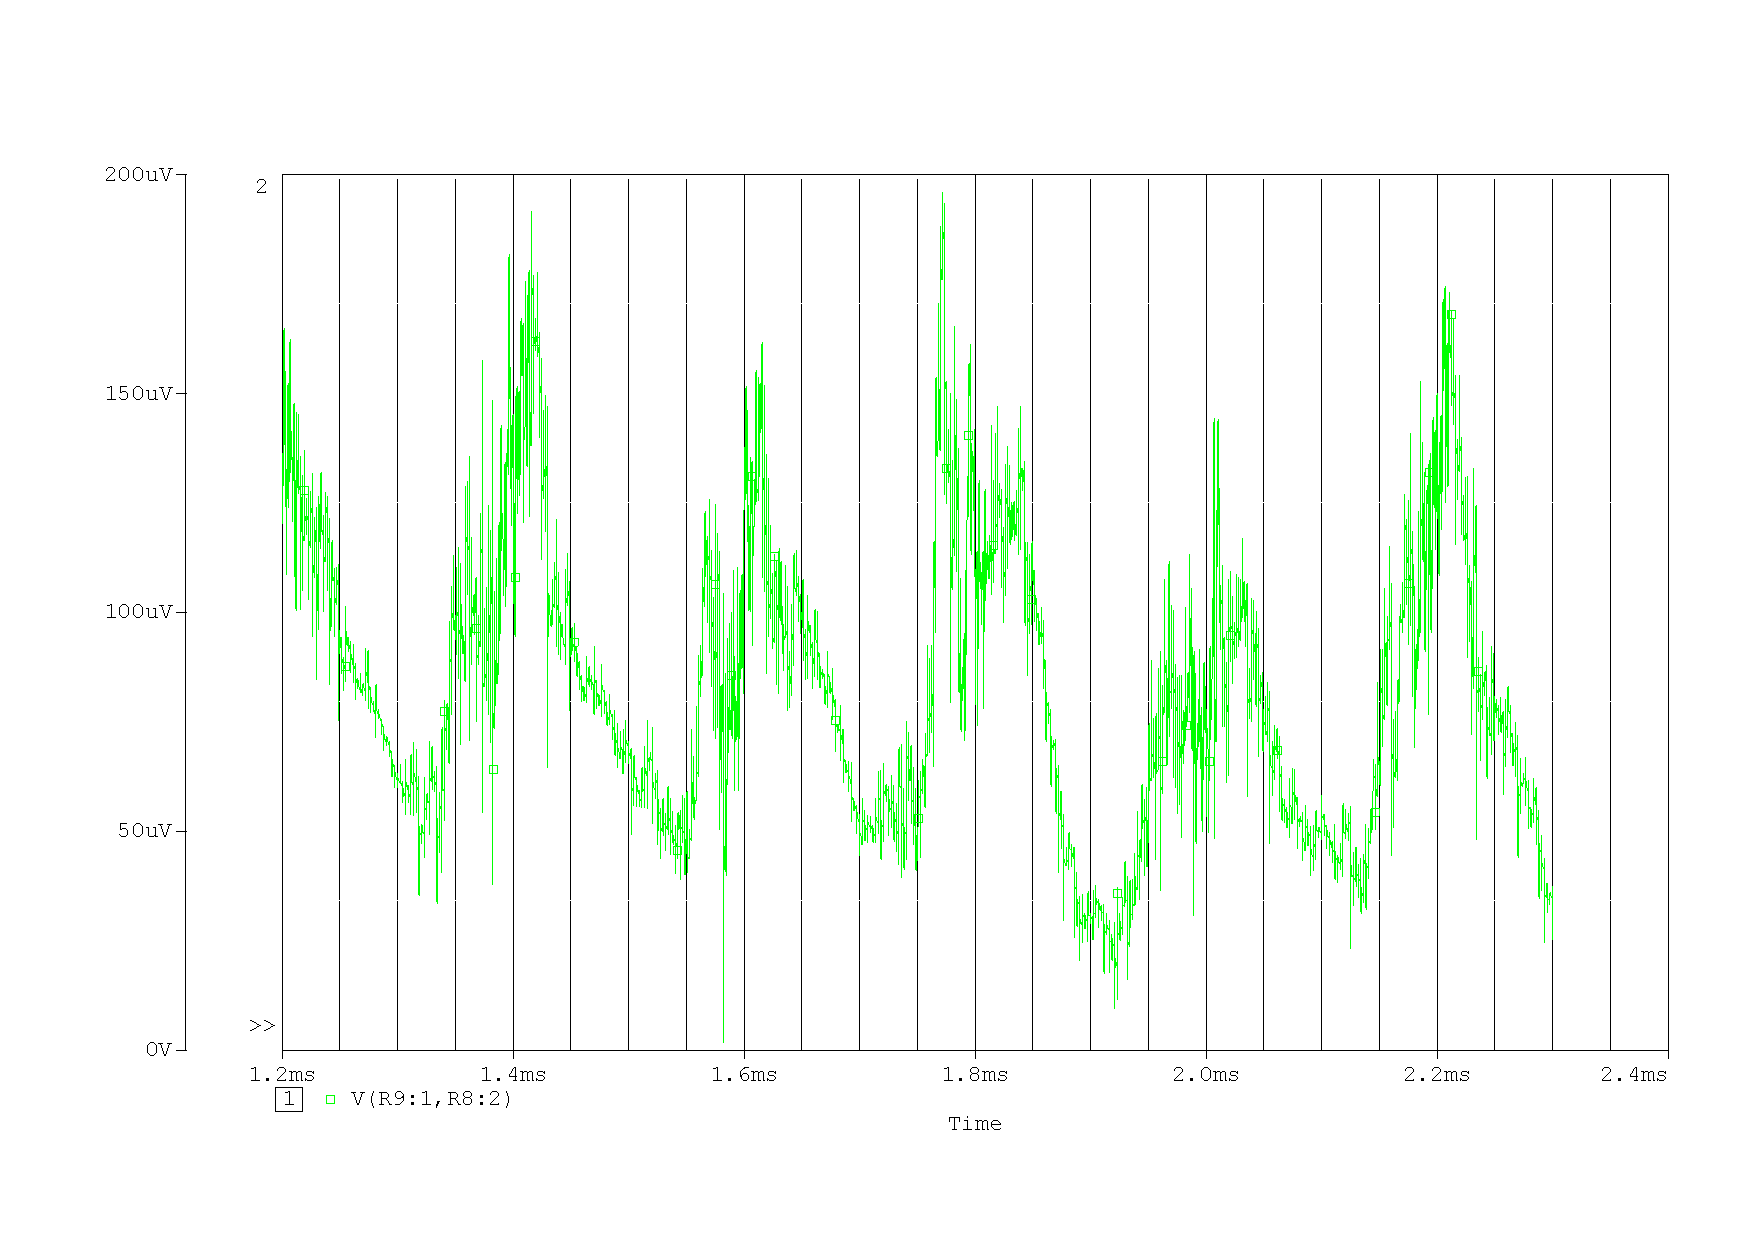
\includegraphics[width=0.43\textwidth]{5k,70MHz.pdf}
    }
     \hspace{0.01\linewidth}
      \subfigure[subfigure 1-2][${v_{o}}_{pp}$=325mV]{
        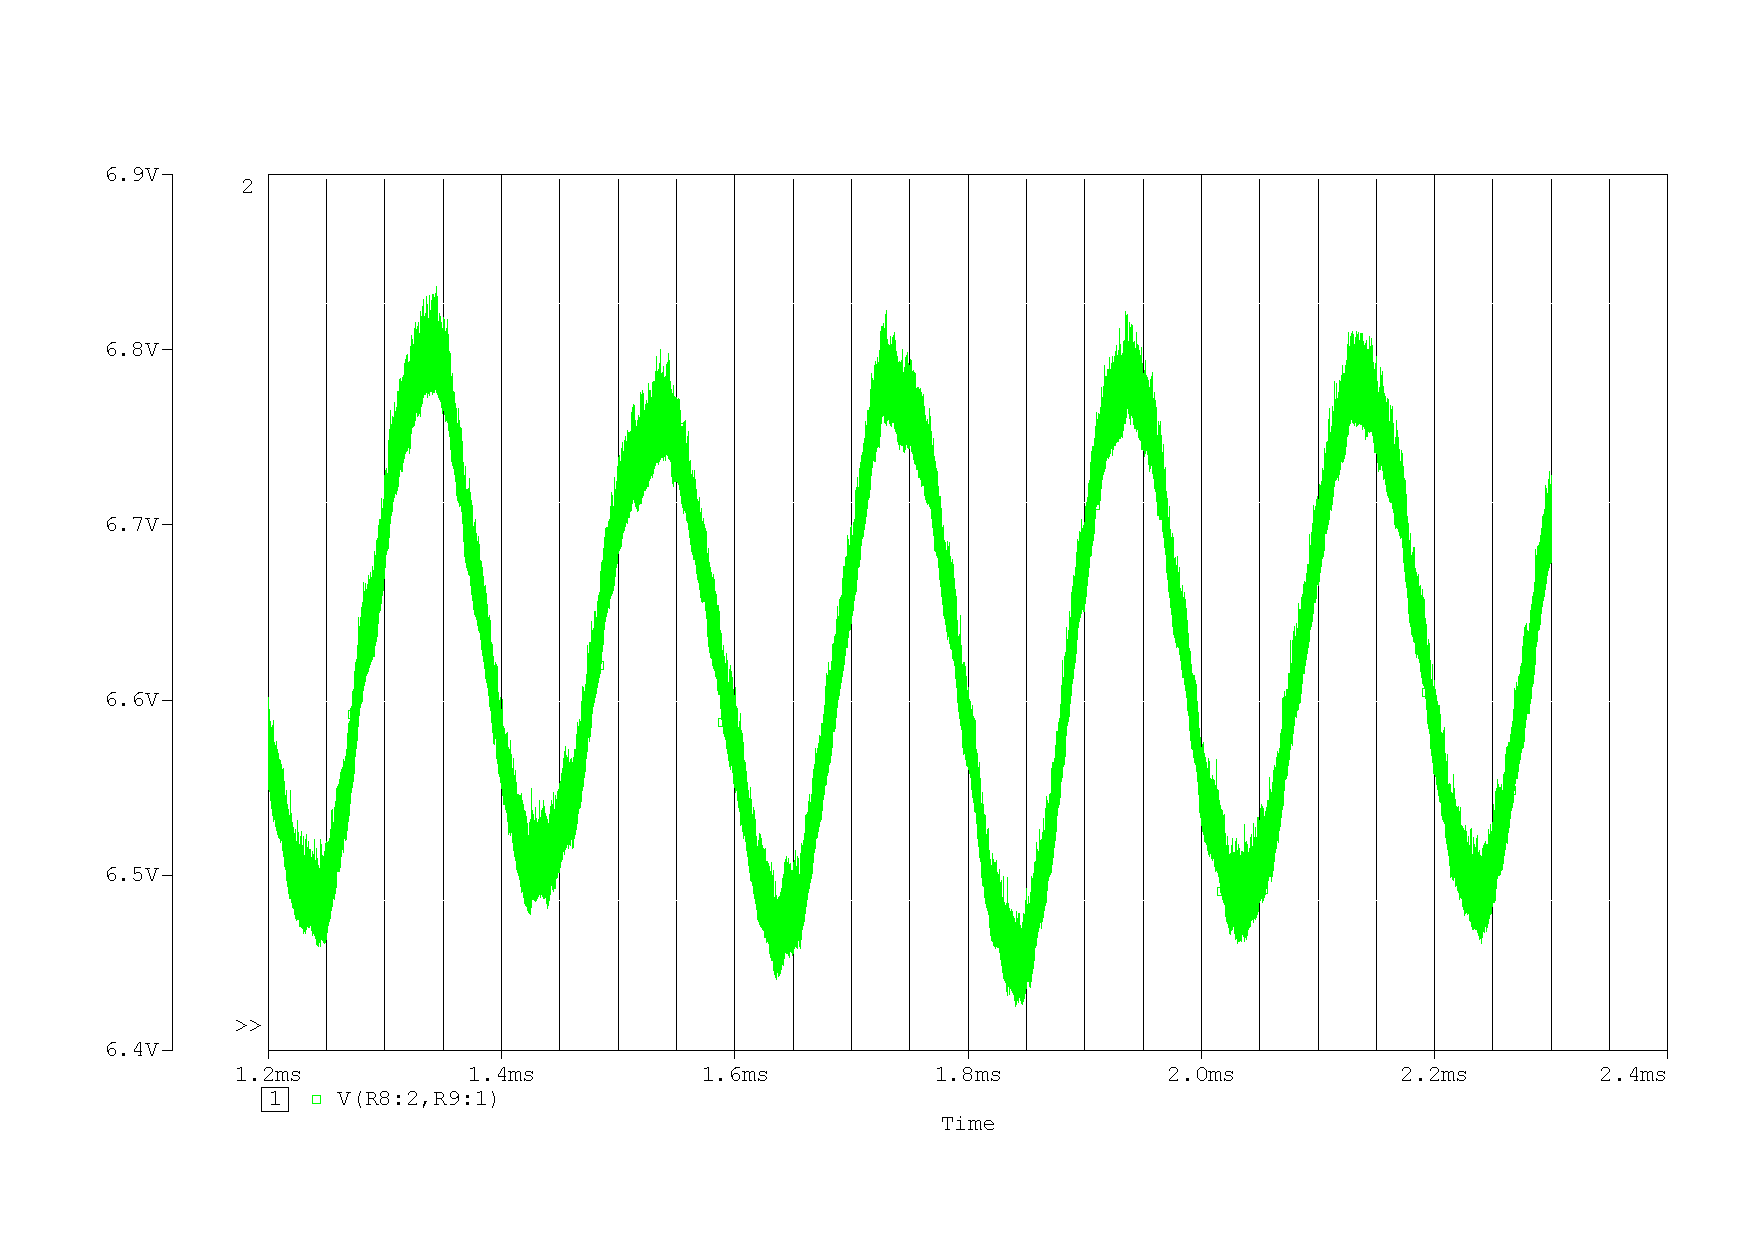
\includegraphics[width=0.43\textwidth]{5k,90MHz.pdf}
    }
     \subfigure[subfigure 1-2][${v_{o}}_{pp}$=330mV]{
        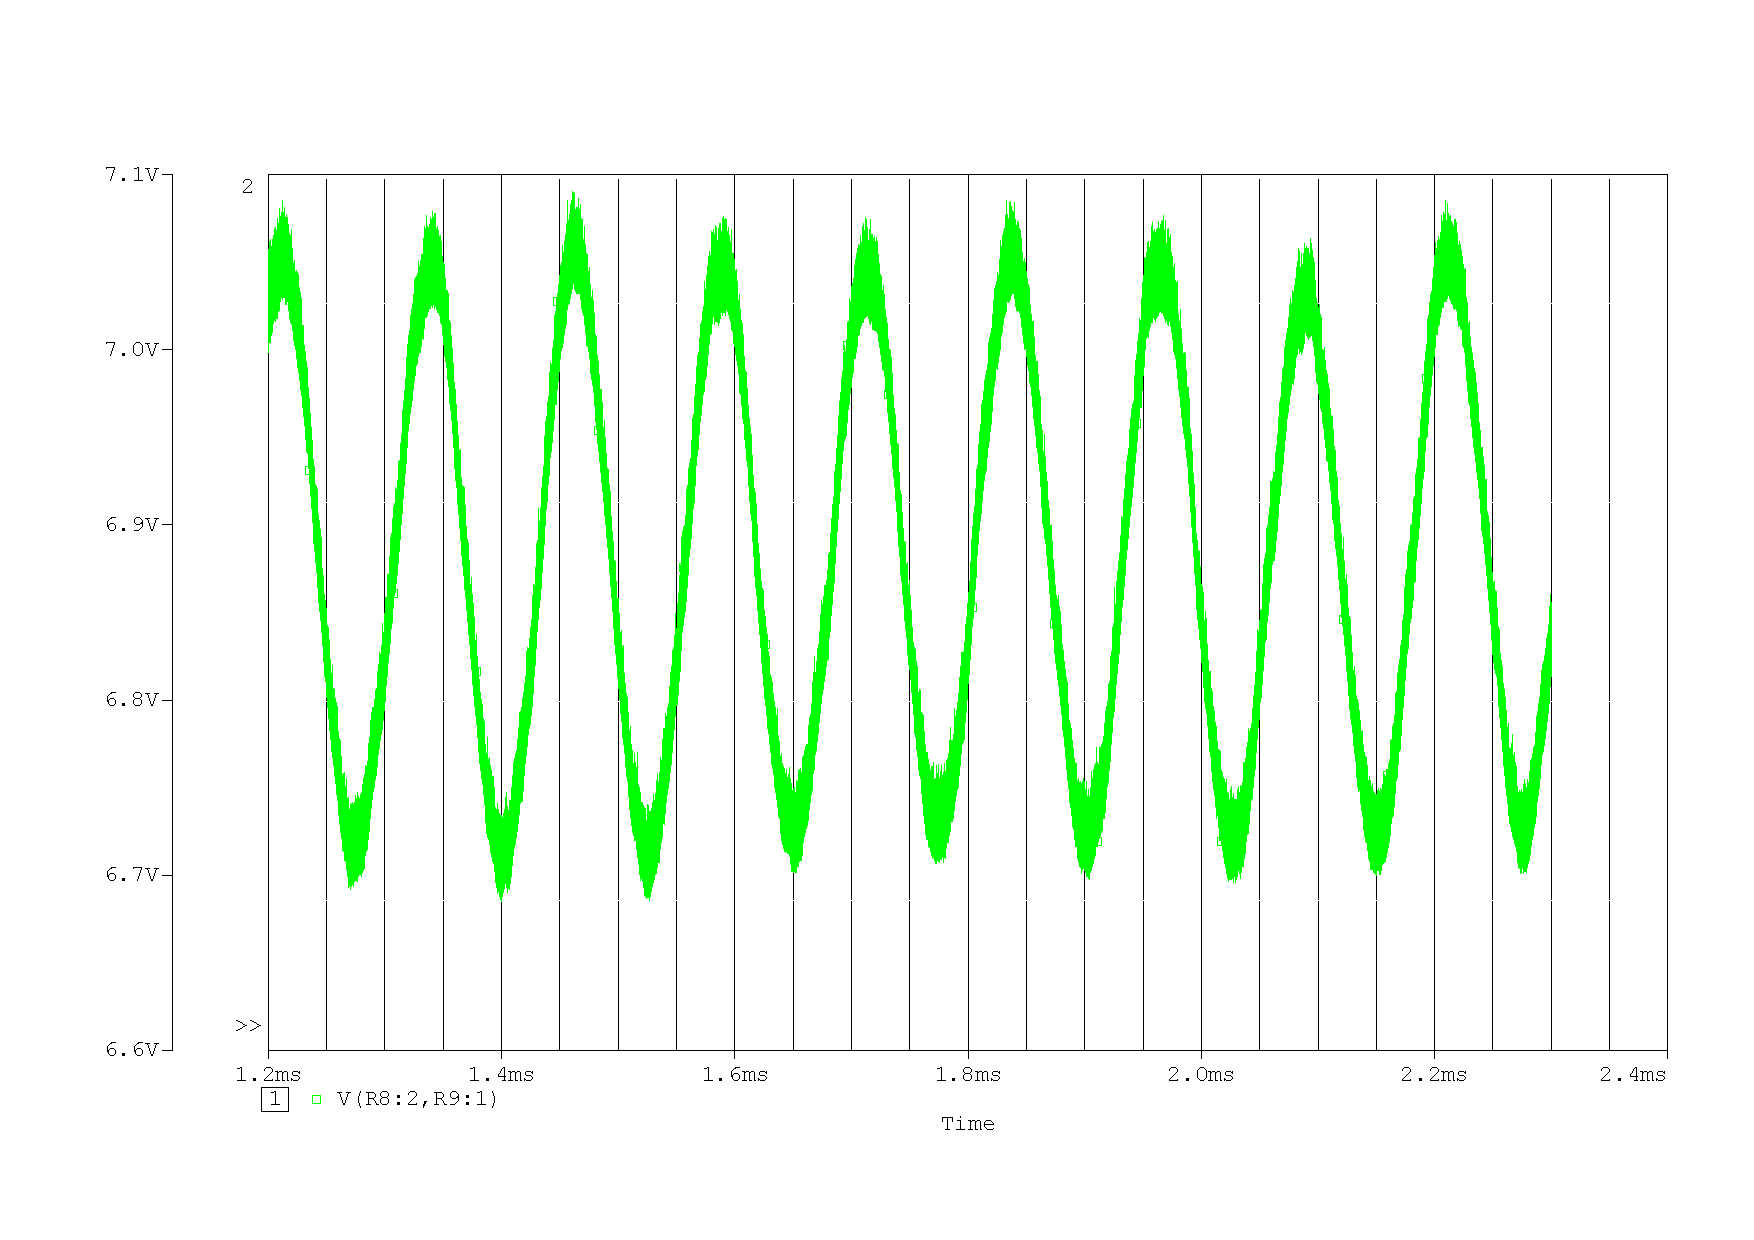
\includegraphics[width=0.43\textwidth]{8k,110MHz.pdf}
    }
     \subfigure[subfigure 1-2][${v_{o}}_{pp}$=16mV]{
        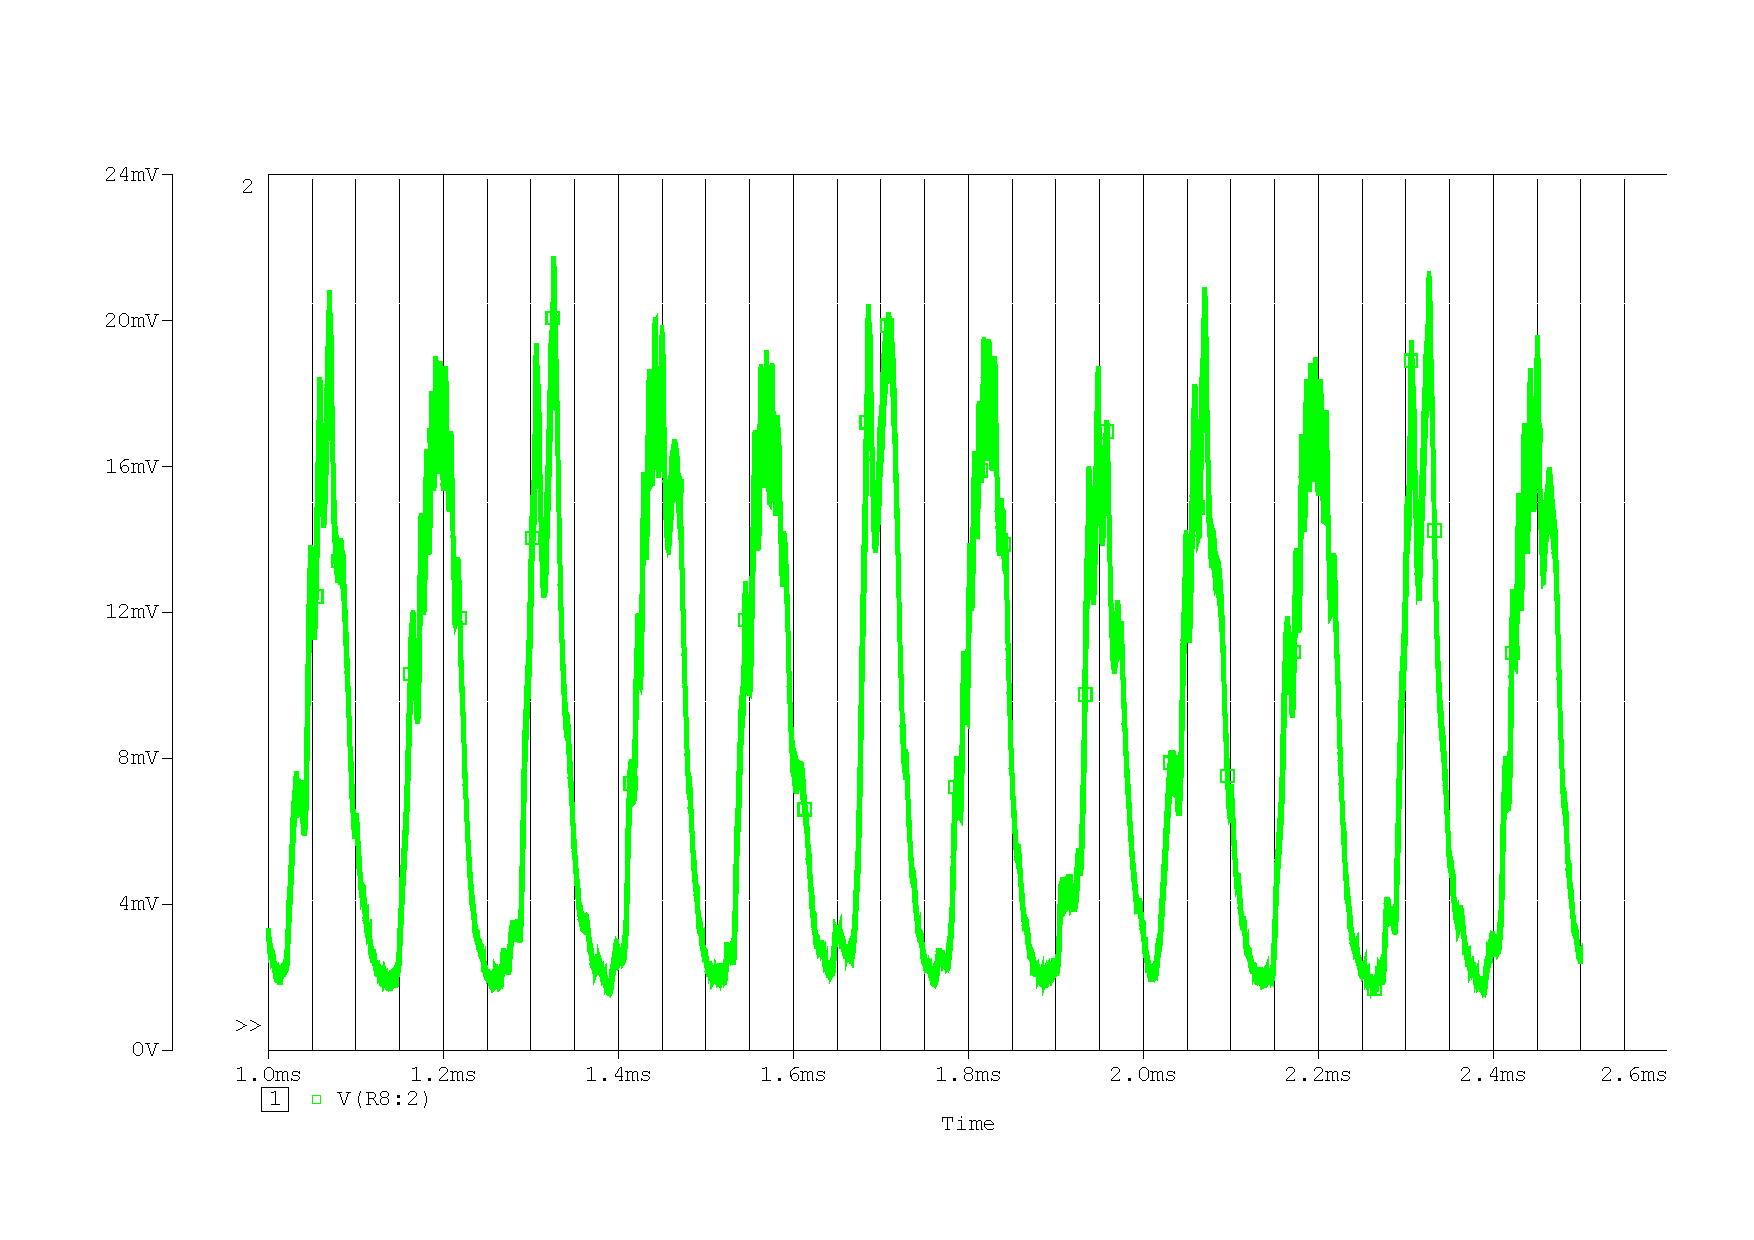
\includegraphics[width=0.43\textwidth]{8k,130MHz.pdf}
    }
    \caption{整机仿真测试组图}
  \label{整机测试结果}
\end{figure}

四组子图(a),(b),(c),(d)分别对应了组1,组2,组3,组4的测试频率。

其中组2及组3(子图b,c)是在工作频率下的输出结果,观察横轴(时间轴),其输出波形均以音频频率对应周期振动,即有效的解调出了音频信号,对纵坐标电压峰峰值进行测量,可知其输出电压均在百毫伏量级,分别为325mV及330mV,波峰及波谷中密集部分是载波频率及中频产生的频率分量,在谐振回路的选频特性及检波过程中已衰减至微伏量级。

组1及组4(子图a,d)是在非工作频率下的输出结果(其中组1以高放级谐振回路谐振于88MHz模拟,组4以高放级谐振回路谐振于108MHz模拟)。观察到波形输出幅度极小,均在100$\mathrm{\mu}$V至10mV的量级,根据一般FM收音机产品标准\cite{调频广播接收机测量方法}\cite{频率范围从87.5至108.0MHz的VHF/FM声音广播无线电数据系统的规范替代BS},没有起到放大音效及扬声的效果;另外,波形产生了明显的上下幅值不对称,高频率分量在波形中的幅值占比也显著增大。

通过四个测试组,可以得出此收音机能够有效地还原出音频信号。对工作频率之内的信号,能够有效地放大音频信号;对工作频率之外的点,通过多级选频作用,信号无法被放大。从而保障了工作频率的稳定性。

\section{总结与体会}
\subsection{设计过程归纳及设计指标参数值归总}
\subsubsection{设计过程归纳}
FM收音机设计过程强调明确各部分电路之间的相互作用,在此基础上再从给定参数出发,着重考虑各部分电路的指标设计问题。对高放级,其输出电压用以放大天线信号并传递至混频电路,因此需要良好的带宽、合适的谐振频率以选出载波及频偏范围内的频率成分,需要恰当的增益使输出幅值不至于过小;对混频级,本机用以稳定混频跨导,因此必须要较高的直流电压使回路工作在大电压状态,需要稳定的频率确保混频频率的稳恒输出,混频器则需要工作在非线性状态,以确保能够成功混频;对中放级,其输出信号对后级解调灵敏度有关键作用,因此首先要设计有较大的增益,其次是恰当的带宽;对解调级,需要足够高的鉴频跨导及足够好的检波能力以确保提取完整的音频信号,因此需要讨论失谐回路的频点及RC回路的充放电时间的选取过程;对低放级,需要确保所有可能频率的音频信号的放大过程,因此需要考虑带宽与增益的设计问题。
\subsubsection{指标参数值归总}
对FM收音机整机设计,本设计报告中主要包含三个方法:公式推导、原理图搭建及仿真模拟,围绕四个主要设计指标:输入载波频率$f_0$,中频$f_I$,声音带宽及灵敏度展开。对高放级,根据式\ref{1式},确定其谐振频点为88MHz-108MHz,根据图\ref{高放频域wave},确定其电压增益为9.426;对混频级,根据式\ref{7式}、图\ref{本振_wave}(a),确保本机振荡器谐振在98.7MHz-118.7MHz之间,根据式\ref{混频跨导}及式\ref{式26},确定混频器混频跨导为0.96S,根据图\ref{混频wave},确保混频器谐振在$f_I$=10.7MHz;对中放级,根据\ref{式18},确定中放级带宽为单调谐回路的0.867倍,根据图\ref{中放_wave}、表\ref{中频测量}、式\ref{式27},确定其功率增益为25.92dB,根据图\ref{中放幅频},确定其带宽为150KHz,满足FM规定最大频偏要求;对解调级,根据式\ref{21式},确定RC时间常数为10$\mathrm{\mu}$s,根据图\ref{解调时域},确定鉴频器成功解调,根据图\ref{解调频域}、图\ref{灵敏度曲线}、式\ref{式28},确定鉴频灵敏度为11.0125$\mathrm{\mu}$V>10$\mathrm{\mu}$V,满足设计要求;对低放级,根据式\ref{式22}、图\ref{低放扫频},确保声音频率范围包含于低放级带宽之内,根据式\ref{效率},确保低频功放效率达70\%以上,根据图\ref{低放时域}及式\ref{式29},确定低放级功率增益为43.6dB。


\subsection{设计体会}
这次设计过程中让我体会到相比掌握收音机的工作原理,在实际的搭建模拟仿真过程中挑战会大得多。有几个仿真细节在设计过程中曾困扰过我一段时间:譬如在尝试用变压器耦合各部分回路时,如何设计K\_linear参数同时耦合多个电感这一问题;在测量混频电路与本机振荡输出波形时,要勾选“跳过瞬态偏置点计算”(SKIPBP);在设计谐振回路时,如何估算次级电感对前级谐振点的干扰,如何预计前级电压耦合到后级的衰减问题等等。这些问题在公式推导甚至理论电原理图的搭建过程中都不会显现出来,尤其在参数设计过程中,晶体管模型的选取也必须要参看器件手册后再做出决定(譬如在低频放大器的上截止频率问题上,晶体管一旦选定就很难通过偏置电阻或旁路电容再对其做出更改)。可以说仿真设计确实有助于加深对元件特性、参数设计过程的认识。



\section{附件A:仿真测试文件对照表}
\begin{table}[H]
    \centering
    \begin{tabular}{ccl}
    \toprule[1.2pt]
    \midrule
      测试电路 & 仿真电路及表笔接入位置 & 文件名 \\
      \midrule
      高频放大电路  & 图\ref{高放时域仿真sch} & HFA.opj \\
        本机振荡电路 & 图\ref{本振仿真电路} & LOCAL\_OSILLATOR.opj \\
        混频电路 & 图\ref{混频仿真电路} & MIXER.opj\\
          中频放大电路 & 图\ref{中放仿真} & IFA.opj\\
          解调电路 & 图\ref{解调仿真电路} &DE\_MODULATION.opj \\
          低频放大电路  & 图\ref{低放仿真电路} & LFA.opj \\
            \bottomrule[1.2pt]
    \end{tabular}
    \caption{FM收音机仿真测试文件对照表}
    \label{仿真文件}
\end{table}

\hspace{2pt} \Large{\textbf{附件B:FM收音机完整电原理/仿真图}}

\normalsize

\begin{itemize}
    \item  FM收音机设计电原理图.pdf
    
    \item  FM收音机仿真整机图.pdf
\end{itemize}  


\printbibliography







\end{document}
